%%%%%% Run at command line, run
%%%%%% xelatex grad-sample.tex 
%%%%%% for a few times to generate the output pdf file
\documentclass[12pt,oneside,openright,a4paper]{cpe-thai-project}
\usepackage{enumitem}
\usepackage{multirow}
\usepackage[table,xcdraw]{xcolor}
\usepackage{float}
\usepackage{url}
\usepackage{graphicx}
\usepackage{makecell}
\usepackage{longtable}
\usepackage{enumitem}
\usepackage{caption}
\usepackage{tikz}
\usepackage{pgfplots}
\usepackage{tabularx}

% \XeTeXlinebreaklocale "th_TH"
% \XeTeXlinebreakskip = 0pt plus 1pt
\usepackage{polyglossia}

\graphicspath{ {./picture/} }

\captionsetup[longtable]{labelfont=bf,labelsep=space,justification=raggedright,singlelinecheck=false}


\setdefaultlanguage{thai}
\setotherlanguage{english}
\newfontfamily\thaifont[Script=Thai,Scale=1.23]{TH Sarabun New}
\defaultfontfeatures{Mapping=tex-text,Scale=1.23,LetterSpace=0.0}
\setmainfont[Scale=1.23,LetterSpace=0,WordSpace=1.0,FakeStretch=1.0]{TH Sarabun New}
% \defaultfontfeatures{Mapping=tex-text,Scale=1.23,LetterSpace=0.0}
% \setmainfont[Scale=1.23,LetterSpace=0,WordSpace=1.0,FakeStretch=1.0]{TH Sarabun New}
%\setmathfont(Digits)[Scale=1.0,LetterSpace=0,FakeStretch=1.0]{Times New Roman}

%%%%%%%%%%%%%%%%%%%%%%%%%%%%%%%%%%%%%%%%%%%%%%%%%%%%%%%%%%%%%%%%%%%
% Customize below to suit your needs 
% The ones that are optional can be left blank. 
%%%%%%%%%%%%%%%%%%%%%%%%%%%%%%%%%%%%%%%%%%%%%%%%%%%%%%%%%%%%%%%%%%%
% First line of title
\def\disstitleone{Project No. 67}   
% Second line of title
\def\disstitletwo{ระบบจัดเก็บและจัดการเอกสารภายในหอบรรณสารสนเทศ }  
% Three line of title
\def\disstitlethree{(KMUTT Archives Management Platform) }   

% Your first name and lastname
\def\dissauthor{Mr.Akarapon Boonsermsakul}   % 1st member
%%% Put other group member names here ..
\def\dissauthortwo{Ms.Thanaporn Pitianusorn}   % 2nd member (optional)
\def\dissauthorthree{Mr.Annop Kongsombatcharoen}   % 3rd member (optional)


% The degree that you're persuing..
\def\dissdegree{Bachelor of Engineering} % Name of the degree
\def\dissdegreeabrev{B.Eng} % Abbreviation of the degree
\def\dissyear{2020}                   % Year of submission
\def\thaidissyear{2563}               % Year of submission (B.E.)

%%%%%%%%%%%%%%%%%%%%%%%%%%%%%%%%%%%%%%%%%%%%
% Your project and independent study committee..
%%%%%%%%%%%%%%%%%%%%%%%%%%%%%%%%%%%%%%%%%%%%
\def\dissadvisor{Asst.Prof. Suthathip Manee, Ph.D.}  % Advisor
%%% Leave it empty if you have no Co-advisor
\def\disscoadvisor{}  % Co-advisor
\def\disscommitteetwo{Dr.Prapong Prechaprapranwong, Ph.D.}  % 3rd committee member (optional)
\def\disscommitteethree{Asst.Prof.Sanan Srakaew}   % 4th committee member (optional) 
\def\disscommitteefour{Asst.Prof.Surapont Toomnark}    % 5th committee member (optional) 

\def\worktype{Project} %%  Project or Independent study
\def\disscredit{3}   %% 3 credits or 6 credits


\def\fieldofstudy{Computer Engineering} 
\def\department{Computer Engineering} 
\def\faculty{Engineering}

\def\thaifieldofstudy{วิศวกรรมคอมพิวเตอร์} 
\def\thaidepartment{วิศวกรรมคอมพิวเตอร์} 
\def\thaifaculty{วิศวกรรมศาสตร์}
 
\def\appendixnames{Appendix} %%% Appendices or Appendix

\def\thaiworktype{ปริญญานิพนธ์} %  Project or research project % 
\def\thaidisstitleone{ระบบจัดเก็บและจัดการเอกสารภายในหอบรรณสารสนเทศ}
\def\thaidisstitletwo{KMUTT Archives Management Platform}
\def\thaidissauthor{นายอัครพล บุญเสริมศักดิ์กุล}
\def\thaidissauthortwo{นางสาวธนพร ปิติอนุสรณ์} %Optional
\def\thaidissauthorthree{นายอรรณพ กองสมบัติเจริญ} %Optional

\def\thaidissadvisor{ผศ.ดร.สุธาทิพย์ มณีวงศ์วัฒนา}
%% Leave this empty if you have no co-advisor
\def\thaidissdegree{วิศวกรรมศาสตรบัณฑิต}

% Change the line spacing here...
\linespread{1.15}

%%%%%%%%%%%%%%%%%%%%%%%%%%%%%%%%%%%%%%%%%%%%%%%%%%%%%%%%%%%%%%%%
% End of personal customization.  Do not modify from this part 
% to \begin{document} unless you know what you are doing...
%%%%%%%%%%%%%%%%%%%%%%%%%%%%%%%%%%%%%%%%%%%%%%%%%%%%%%%%%%%%%%%%


%%%%%%%%%%%% Dissertation style %%%%%%%%%%%
%\linespread{1.6} % Double-spaced  
%%\oddsidemargin    0.5in
%%\evensidemargin   0.5in
%%%%%%%%%%%%%%%%%%%%%%%%%%%%%%%%%%%%%%%%%%%
%\renewcommand{\subfigtopskip}{10pt}
%\renewcommand{\subfigbottomskip}{-5pt} 
%\renewcommand{\subfigcapskip}{-6pt} %vertical space between caption
%                                    %and figure.
%\renewcommand{\subfigcapmargin}{0pt}

\renewcommand{\topfraction}{0.85}
\renewcommand{\textfraction}{0.1}

\newtheorem{theorem}{Theorem}
\newtheorem{lemma}{Lemma}
\newtheorem{corollary}{Corollary}
\setlength{\parskip}{1em}

\def\QED{\mbox{\rule[0pt]{1.5ex}{1.5ex}}}
\def\proof{\noindent\hspace{2em}{\itshape Proof: }}
\def\endproof{\hspace*{\fill}~\QED\par\endtrivlist\unskip}
%\newenvironment{proof}{{\sc Proof:}}{~\hfill \blacksquare}
%% The hyperref package redefines the \appendix. This one 
%% is from the dissertation.cls
%\def\appendix#1{\iffirstappendix \appendixcover \firstappendixfalse \fi \chapter{#1}}
%\renewcommand{\arraystretch}{0.8}
%%%%%%%%%%%%%%%%%%%%%%%%%%%%%%%%%%%%%%%%%%%%%%%%%%%%%%%%%%%%%%%%
%%%%%%%%%%%%%%%%%%%%%%%%%%%%%%%%%%%%%%%%%%%%%%%%%%%%%%%%%%%%%%%%
\begin{document}
\pdfstringdefDisableCommands{%
\let\MakeUppercase\relax
}
\begin{center}

\includegraphics[width=2.8cm]{logo02.jpg}
\end{center}
\vspace*{-1cm}
\maketitlepage
\makesignaturepage 
% Prevent hyphens to show up in texts
\XeTeXlinebreaklocale "th"	
\emergencystretch=10pt %allows some extra whitespace per line.
%%%%%%%%%%%%%%%%%%%%%%%%%%%%%%%%%%%%%%%%%%%%%%%%%%%%%%%%%%%%%%
%%%%%%%%%%%%%%%%%%%%%% English abstract %%%%%%%%%%%%%%%%%%%%%%%
%%%%%%%%%%%%%%%%%%%%%%%%%%%%%%%%%%%%%%%%%%%%%%%%%%%%%%%%%%%%%%
\abstract

KMUTT's library have collected the archive of valued documents. 
Because these document have not transformed into digital form, 
there is vital problem in searching for information in these 
document for librarian and patrons. In this project, we developed 
web platform to digitize these document into digital format 
and implement the search function that facilitate the librarian 
and patron to search for information. The platform consists of 
2 components. The first part is importing documents and 
digitization. In this step, we applied image processing 
techniques such as Morphology Transformation to preprocess
the images of documents and transform the images to full text 
data by using Tesseract. After getting the text files, we tokenize 
the text into words by using the Deepcut library and find the 
significant words of the document by using the TF-IDF algorithm. 
In the second part, we start by getting the input from the user 
and use the word2Vec model to find a similar word. And take 
input and similar words to get the TF-IDF score that we 
generate at first to find the best document for the input word.  

Comparing the result between using OCR and using OCR with correction system, 
using only OCR have correction score around 74.75 percents and using OCR with correction system
have correction score 76.61 percents.

And the accuracy and recall of search system without Word2Vec are 75 percents and 88.24 percents accordingly.
But after using Word2Vec models the accuracy drop to 61.45 percents while recall is still the same as without Word2Vec.

\begin{flushleft}
\begin{tabular*}{\textwidth}{@{}lp{0.8\textwidth}}
\textbf{Keywords}: & Natural language processing / RESTful Service / Optical character recognition / Image Processing / Information retrieval / Term Frequency-Inverse Document Frequency / Word2Vec / Word Embedded 
\end{tabular*}
\end{flushleft}
\endabstract

%%%%%%%%%%%%%%%%%%%%%%%%%%%%%%%%%%%%%%%%%%%%%%%%%%%%%%%%%%%%%%
%%%%%%%%%% Thai abstract here %%%%%%%%%%%%%%%%%%%%%%%%%%%%%%%%%
%%%%%%%%%%%%%%%%%%%%%%%%%%%%%%%%%%%%%%%%%%%%%%%%%%%%%%%%%%%%%%
% {\newfontfamily\thaifont{TH Sarabun New:script=thai}[Scale=1.3]
% \XeTeXlinebreaklocale "th_TH"	
% \thaifont
\thaiabstract

การจะสืบค้นข้อมูลจากเอกสารหรือชั้นหนังสือที่มีการรวบรวมข้อมูลไว้ตั้งแต่อดีตนั้นเป็น
ปัญหาอย่างหนึ่งของเจ้าหน้าที่บรรณารักษ์ที่ต้องทำการดูแลเอกสารเหล่านี้ เนื่องจาก
การที่ยังไม่มีการเก็บหนังสือและเอกสารให้อยู่ในรูปแบบของข้อมูลดิจิทัลทำให้ต้อง
สืบค้นโดยการค้นหาเอกสารและหนังสือแต่ละเล่มโดยการดูจากเนื้อหาสารบัญเพื่อให้
ได้หนังสือที่ตรงกับข้อมูลที่ต้องการมากที่สุด ซึ่งการที่ค้นหาจากหน้าสารบัญของ
หนังสือแต่ละเล่มก็จะทำให้การค้นหาเป็นไปอย่างล่าช้า และบางครั้งการดูเพียง
แค่สารบัญก็อาจจะทำให้ได้หนังสือที่ไม่ตรงกับความต้องการของผู้ที่เข้ามายืมหนังสือ 
ในโครงการนี้เราได้ทำการพัฒนาการระบบจัดเก็บและค้นหาเอกสารอิเล็กทรินิกส์ 
โดยแบ่งออกเป็น 2 ขั้นตอนคือ การนำเข้าข้อมูล  และการสร้างระบบค้นหา 
โดยขั้นตอนการนำเข้าข้อมูล เราจะเริ่มจากการเตรียมข้อมูลรูปภาพ
เพื่อเตรียมข้อมูลรูปภาพที่ได้มา ก่อนจะนำไปผ่านกระบวนการ OCR 
เพื่อแปลงรูปภาพเหล่านี้ให้อยู่ในรูปของข้อมูลดิจิทัล โดยการเก็บข้อมูลในรูปแบบของ 
Information Retrieval เพื่อช่วยให้ความเร็วการค้นหามีประสิทธิภาพมากยิ่งขึ้น 
และนำข้อมูลมาทำการตัดคำ และเช็คคำผิด จากนั้นจะนำมาหาคำสำคัญของหนังสือหรือเอกสารนั้น ๆ
โดยการใช้การหาคะแนนแบบ TF-IDF ส่วนการสร้างระบบการค้นหาจะเริ่มจากรับคำค้นหามาจากผู้
ใช้และทำการนำคำที่ได้ไปเข้าโมเดล word2Vec เพื่อหาคำที่ใกล้เคียง 
จากนั้นนำคำใกล้เคียงและคำค้นหาไปดึงคะแนน TF-IDF ที่เก็บไว้เพื่อค้นหาว่า
มีเอกสารหรือหนังสือเล่มไหนที่มีคะแนนที่ตรงและใกล้เคียงกับคำค้นหามากที่สุด
โดยผลลัพธ์จากการทำ OCR ถูกต้อง 74.75 \%และเมื่อนำมาผ่านกระบวนการแก้คำผิดได้ความถูกต้องอยู่ที่ 76.61\%
และมีผลลัพธ์ในการค้นหาโดยที่ไม่ใช้ Word2Vec มีความแม่นยำอยู่ที่ 75 \% และความครอบคลุมอยู่ที่ 88.24 \% 
แต่หลังจากใช้งาน Word2Vec มีความแม่นยำอยู่ที่ 61.45 \% และความครอบคลุมอยู่ที่ 88.24 \%
\begin{flushleft}
\begin{tabular*}{\textwidth}{@{}lp{0.8\textwidth}}
 & \\

\textbf{คำสำคัญ}: & Natural language processing / RESTful Service / Optical character recognition / Image Processing / Information retrieval / Term Frequency-Inverse Document Frequency / Word2Vec / Word Embedded 
\end{tabular*}
\end{flushleft}
\endabstract
% }

%%%%%%%%%%%%%%%%%%%%%%%%%%%%%%%%%%%%%%%%%%%%%%%%%%%%%%%%%%%%
%%%%%%%%%%%%%%%%%%%%%%% Acknowledgments %%%%%%%%%%%%%%%%%%%%
%%%%%%%%%%%%%%%%%%%%%%%%%%%%%%%%%%%%%%%%%%%%%%%%%%%%%%%%%%%%
\preface
ขอขอบคุณนางสาวอารยา ศรีบัวบาน เจ้าหน้าที่หอบรรณสารสนเทศและ ผศ.ดร.สุธาทิพย์ มณีวงศ์วัฒนา อาจารย์ที่ปรึกษารวมทั้งเจ้าหน้าที่ภาย
ในหอสมุดมหาวิทยาลัยเทคโนโลยีพระจอมเกล้าธนบุรีที่เสียสละเวลาให้ความรู้ความเข้าใจ ทั้งในเรื่องการเก็บข้อมูลและคอยแนะนำวิธีการจัดการกับ
ปัญหาต่างๆที่เกิดขึ้น นำมาสู่การทำหัวข้อปริญญานิพนธ์ฉบับนี้ให้สำเร็จตามที่ต้องการ 

%%%%%%%%%%%%%%%%%%%%%%%%%%%%%%%%%%%%%%%%%%%%%%%%%%%%%%%%%%%%%
%%%%%%%%%%%%%%%% ToC, List of figures/tables %%%%%%%%%%%%%%%%
%%%%%%%%%%%%%%%%%%%%%%%%%%%%%%%%%%%%%%%%%%%%%%%%%%%%%%%%%%%%%
% The three commands below automatically generate the table 
% of content, list of tables and list of figures
\tableofcontents                    
\listoftables
\listoffigures                      

%%%%%%%%%%%%%%%%%%%%%%%%%%%%%%%%%%%%%%%%%%%%%%%%%%%%%%%%%%%%%%
%%%%%%%%%%%%%%%%%%%%% List of symbols page %%%%%%%%%%%%%%%%%%%
%%%%%%%%%%%%%%%%%%%%%%%%%%%%%%%%%%%%%%%%%%%%%%%%%%%%%%%%%%%%%%
% You have to add this manually..
% \listofsymbols
% \begin{flushleft}
% \begin{tabular}{@{}p{0.07\textwidth}p{0.7\textwidth}p{0.1\textwidth}}
% \textbf{SYMBOL}  & & \textbf{UNIT} \\[0.2cm]
% $\alpha$ & Test variable\hfill & m$^2$ \\
% $\lambda$ & Interarival rate\hfill &  jobs/second\\
% $\mu$ & Service rate\hfill & jobs/second\\
% \end{tabular}
% \end{flushleft}
%%%%%%%%%%%%%%%%%%%%%%%%%%%%%%%%%%%%%%%%%%%%%%%%%%%%%%%%%%%%%%
%%%%%%%%%%%%%%%%%%%%% List of vocabs & terms %%%%%%%%%%%%%%%%%
%%%%%%%%%%%%%%%%%%%%%%%%%%%%%%%%%%%%%%%%%%%%%%%%%%%%%%%%%%%%%%
% You also have to add this manually..

% \listofvocab
% \begin{flushleft}
% \begin{tabular}{@{}p{1in}@{=\extracolsep{0.5in}}l}
% API &   \\
% CNN & Convolutional Neural Network \\
% ER & Entity Relationship \\
% FK & Foreign Key \\
% IDF & Inverse Document Frequency \\
% INT & Interger \\
% IR & Information Retrieval \\
% JWT & JSON Web Token \\
% LSTM & Long Short Term Memory \\
% MVC & Model View Controller \\
% NLP & Natural Language Processing \\
% NLTK & \\ 
% OCR & Optical Character Recognization \\
% OpenCV & \\
% PDF & \\
% PK & Primary Key \\
% TF & Term Frequency \\
% UI & User Interface \\
% UX & User Experience \\

% \end{tabular}
% \end{flushleft}

%\setlength{\parskip}{1.2mm}

%%%%%%%%%%%%%%%%%%%%%%%%%%%%%%%%%%%%%%%%%%%%%%%%%%%%%%%%%%%%%%%
%%%%%%%%%%%%%%%%%%%%%%%% Main body %%%%%%%%%%%%%%%%%%%%%%%%%%%%
%%%%%%%%%%%%%%%%%%%%%%%%%%%%%%%%%%%%%%%%%%%%%%%%%%%%%%%%%%%%%%%
\chapter{บทนำ}

\section{คำสำคัญ}

Natural language processing, RESTful Service, Optical character recognition, Image Processing, Information retrieval, Term Frequency-Inverse Document Frequency, Word2Vec, Word Embedded 

\section{ความสำคัญของปัญหา}

นับตั้งแต่การก่อตั้งหอสมุดมหาวิทยาลัยเทคโนโลยีพระจอมเกล้าธนบุรี ได้มีการเก็บรวบรวมองค์ความรู้จากประสบการณ์การทำงานของคณะอาจารย์ ผู้เชี่ยวชาญในทางด้านศาสตร์ต่าง ๆ ในรูปแบบลายมือและสื่อสิ่งพิมพ์ไม่ว่าจะเป็น หนังสือ หนังสือ รวมถึงบันทึกเหตุการณ์ในอดีตในรูปของจดหมายเหตุเพื่อส่งต่อประวัติศาสตร์ความรู้ไปยังคนรุ่นหลังโดยมีการจัดเก็บอยู่ภายในหอจดหมายเหตุที่มีเจ้าหน้าที่บรรณารักษ์เป็นผู้ดูแล และเนื่องจากการที่ หนังสือ หนังสือยังไม่ได้มีการจัดเก็บในรูปแบบดิจิทัลทำให้เมื่อมีบุคคลภายนอกที่ต้องการข้อมูลเพื่อนำไปทำกิจกรรมต่าง ๆ ไม่ว่าจะเป็นการทำวิจัย รายงาน หรือหาข้อมูลเพื่อประกอบการประชุมก็ตามแต่ ก็จำเป็นที่จะต้องมาติดต่อเจ้าหน้าที่บรรณารักษ์ผู้ดูแลเพื่อที่จะให้เจ้าหน้าที่บรรณารักษ์ทำการค้นหาหนังสือที่มีเนื้อหาตามที่เราต้องการ ซึ่งการค้นหาข้อมูลที่ต้องการนั้นเจ้าหน้าที่จะต้องทำการค้นหาด้วยระบบมือทำให้การค้นหาข้อมูลดำเนินการไปอย่างล่าช้า นอกจากนั้นวิธีการหาข้อมูลของเจ้าหน้าที่บรรณารักษ์จะเลือกตรวจสอบข้อมูลของหนังสือจากการดูสารบัญทำให้ข้อมูลที่ได้รับมาอาจจะตกหล่นจากข้อมูลเล่มอื่นได้ 

เพื่ออำนวยความสะดวกให้กับบรรณารักษ์ในการสืบค้นข้อมูลและทำให้การบริการในการสืบค้นหนังสือต่าง ๆ และให้บุคคลภายนอกสามารถทำการค้นหาข้อมูลได้ด้วยตนเองครบถ้วนทางคณะผู้จัดทำโครงการจึงได้พัฒนาระบบการจัดเก็บหนังสือและระบบการค้นหาโดยการใช้เครื่องมือในการทำ OCR เพื่อแปลงหนังสือให้อยู่ในรูปแบบของหนังสือ ดิจิทัล และหาคำสำคัญในการสร้างแท็ก ด้วยวิธี Term Frequency - Inverse Document Frequency เพื่อเพิ่มประสิทธิ์ภาพให้กับการค้นหา 

\section{ประเภทของโครงงาน}

นำเสนอความต้องการของผู้มีส่วนได้ส่วนเสียเฉพาะกลุ่ม 

\section{วิธีการที่นำเสนอ}

ระบบการค้นหาหนังสือ มีขั้นตอนการทำงานดังนี้

\begin{enumerate}
    \item นำหนังสือมาแปลงเป็นรูปภาพในรูปแบบสแกน
    \item นำรูปภาพเข้าสู่ระบบโดยใช้การรับส่งข้อมูลแบบ RESTful API ในระบุประเภทของการใช้งาน
    \item นำรูปภาพผ่านกระบวนการเตรียมข้อมูลรูปภาพ โดยใช้ OpenCV ในการลบส่วนอื่น ๆที่ไม่ใช่ข้อความออกและตัดเฉพาะข้อความเพื่อนำไปใช้ในขั้นต่อไป
    \item นำรูปที่ผ่านการเตรียมข้อมูลรูปภาพ มาเข้าสู่ระบบ OCR เพื่อแปลงข้อมูลจากรูปภาพมาเป็นข้อความในระบบดิจิทัล
    \item นำข้อมูลที่เก็บไว้มาทำการตัดแบ่งคำภาษาไทยและแก้คำผิด
    \item ค้นหาคำสำคัญโดยใช้วิธี TF-IDF เพื่อนำมาใช้ในการสร้างแท็ก 
    \item นำข้อมูลที่ถูกแปลงเก็บและข้อมูลเกี่ยวกับแท็ก ลงในดาต้าเบส 
    \item ทำระบบค้นหาในรูปแบบโคซายซิมิลาริตี้(Cosine Similarity) 
    \item ทำระบบหาคำใกล้เคียงโดยใช้วิธี Word2Vec
    \item ทำแพลตฟอร์มเว็ปไซต์เพื่อเป็น User Interface ให้กับผู้ใช้งานได้ใช้งานสำหรับการใช้งานในการค้นหาข้อมูลและเพิ่มข้อมูลหนังสือลงไปในฐานข้อมูลเพิ่ม
\end{enumerate}
\section{วัตถุประสงค์}
\begin{enumerate}
    \item สร้างระบบแปลงข้อมูลหนังสือให้อยู่ในรูปแบบดิจิทัล
    \item สร้าง web platform เพื่อทำการค้นหาหนังสือจากคำค้น และพัฒนาเครื่องมือสนับสนุนการทำงานของบรรณารักษ์ประจำหอบรรณสารสนเทศ
    \item สร้างระบบการค้นหาโดยการใช้วิธีการ อินฟอเมชันรีทีฟวอล ซึ่งวัดความใกล้เคียงกันระหว่างคำค้นและข้อมูลในฐานข้อมูลโดยวิธีโคซายซิมิลาริตี้(Cosine Similarity)
    \item เพิ่มประสิทธิ์ภาพในการเข้าถึงข้อมูลในรูปแบบดิจิทัล
    \item เรียนรู้เรื่องการเตรียมข้อมูลรูปภาพ
\end{enumerate}
\section{ขอบเขตของงานวิจัย}
\begin{enumerate}
    \item ระบบแปลงข้อมูลจากหนังสือและหนังสือเก่า รองรับเฉพาะหนังสือที่เป็นตัวอักษรแบบพิมพ์ และรองรับไฟล์หนังสือเฉพาะ PDF เท่านั้น
    \item ทำระบบตัดคำ Stop word ภาษาไทยโดยอ้างอิงมาจาก pythainip และภาษาอังกฤษจาก nltk
    \item ทำระบบค้นหาแบบโคซายซิมิลาริตี้(Cosine Similarity) ในระบบ Information retrieval
    \item ข้อมูลหนังสือที่นำมาใช้คือหนังสือจำพวก งานแสดงกตเวทิตาจิต หนังสือรายงานประจำปี ตั้งแต่ปีพุทธศักราช 2527 ถึง 2560 รวมประมาณ 43 เล่ม จากหอจดหมายเหตุมหาวิทยาลัยเทคโนโลยีพระจอมเกล้าธนบุรี
    \item ทำ platform เว็บไซต์ในรูปแบบ responsive แต่ไม่รองรับขนาดมือถือ รองรับเฉพาะคอมพิวเตอร์หรือโน๊ตบุ๊ค
    \item การแปลงสิ่งพิมพ์เป็นดิจิทัลใช้ Tesseract ในการแปลงหนังสือและหนังสือเป็นรูปแบบดิจิทัล
    \item การตัดคำภาษาไทยทางคณะผู้จัดทำ จะใช้ freeware เช่น DeepCut มาใช้ในส่วนของการตัดคำภาษาไทย
\end{enumerate}
\section{เนื้อหาทางวิศวกรรมที่เป็นต้นฉบับ}
\begin{itemize}
    \item การเตรียมข้อมูลรูปภาพ สำหรับการเตรียมภาพก่อนนำไปทำ OCR 
    
    โปรเจคของเราทำเกี่ยวกับการทำ OCR เพื่ออ่านภาพให้กลายเป็น text แต่ถึงแม้ว่าภาพที่ได้มาจะจากการสแกนหรือการถ่ายรูป แต่ถึงอย่างนั้น OCR ที่ใช้ก็ยังคงมีข้อจำกัดในเรื่องของคุณภาพของภาพที่ใช้ ถ้าเกิดว่าภาพที่ใช้เอียง หรือมี noise จะทำให้การอ่านมีประสิทธิภาพน้อยลง นอกจากนี้การตัดภาพแยกย่อหน้าแต่ละย่อหน้าทำให้การอ่านมีความถูกต้องมากยิ่งขึ้น

    \item การพัฒนาเว็บไซต์สำหรับการค้นหาหนังสือในหอจดหมายเหตุ
    
    เว็บไซต์ของเราจะใช้ ReactJS, NodeJs, python  ในการพัฒนาเว็บไซต์เป็น Interface ให้กับผู้ใช้งาน สำหรับการใช้งานระบบการค้นหาหนังสือ รวมถึงการอัปโหลดหนังสือเพื่อแปลงหนังสือเข้าสู่ระบบดิจิทัลและ API ต่าง ๆ
    
    \item คัดเลือกคำสำคัญออกมาเพื่อสร้างแท็ก 
    
    สำหรับแบ่งแยกหมวดหมู่ของหนังสือโดยใช้ หลักการของ TF-IDF ในการค้นหาคำสำคัญของหนังสือเพื่อนำมาสร้างแท็ก และใช้สำหรับการค้นหาข้อมูล
    
    \item ทำระบบค้นหาโดยใช้คำที่มีความหมายใกล้เคียง
    
    สำหรับการค้นหาเราจะนำคะแนน TF-IDF มาใช้เป็นคะแนนเพื่อใช้ในการค้นหาแบบโคซายซิมิลาริตี้(Cosine Similarity) และค้นหาคำใกล้เคียง (Query Expansion) เพื่อทำให้การค้นหาเจอผลลัพธ์ที่ต้องการเพิ่มมากขึ้น
    
\end{itemize}
\section{การแยกย่อยงาน และร่างแผนการดำเนินงาน}
\begin{enumerate}
    \item 	ศึกษาและค้นคว้าปัญหาของโครงการ
    \item 	เสนอหัวข้อโปรเจค 
    \item 	ค้นหาข้อมูลเกี่ยวกับเทคโนโลยีที่ใช้ในโปรเจค
    \item 	ประเมินความเป็นไปได้และกำหนดขอบเขตของโปรเจค 
    \item 	จัดเก็บ requirement จากกลุ่มผู้ใช้งาน
    \begin{enumerate}[label*=\arabic*.]
        \item   ติดต่อเจ้าหน้าที่ของหอสมุด
        \item   เก็บข้อมูลที่ต้องการแปลงเข้าสู่ระบบดิจิทัล
    \end{enumerate}
    \item 	นำเสนอโครงการครั้งที่ 1 
    \item 	ออกแบบ UX/UI
    \item 	การแปลงรูปภาพให้อยู่ในรูปแบบดิจิทัล
    \begin{enumerate}[label*=\arabic*.]
        \item  นำหนังสือมาแปลงเป็นรูปภาพในรูปแบบสแกน 
        \item  ศึกษาการใช้งาน OpenCV
        \item  สร้างระบบการเตรียมข้อมูลรูปภาพ เพื่อทำการปรับแต่งรูปภาพและทำการปรับแต่งจนได้ระบบที่รองรับกับ Data ที่มี
        \item  นำรูปที่ผ่านการเตรียมข้อมูลรูปภาพ มาเข้าสู่ระบบ OCR เพื่อแปลงข้อมูลจากรูปภาพมาเป็นข้อความในระบบดิจิทัล 
    \end{enumerate}
    \item 	นำข้อมูลที่เก็บไว้มาทำการตัดแบ่งคำภาษาไทยและหาคำสำคัญโดยใช้ TF-IDF 
    \begin{enumerate}[label*=\arabic*.]
        \item	ทำการตัดแบ่งคำ (Tokenization)
        \item	ลบ stop word ออกจากข้อมูล 
    \end{enumerate}
    \item	ทำระบบค้นหา 
    \begin{enumerate}[label*=\arabic*.]
       \item	ทำระบบค้นหาโดยใช้หลักการโคซายซิมิลาริตี้(Cosine Similarity)
       \item	ทำการค้นหาด้วยคำใกล้เคียงโดยใช้ Word2Vec 
    \end{enumerate}    
    \item   จัดทำเว็บไซต์แพลตฟอร์ม
    \item   ทดสอบระบบ
    \item   ปรับปรุงแก้ไข
    \item   นำเสนอโปรเจค
    \end{enumerate}

\section{ตารางการดำเนินงาน}

\renewcommand{\arraystretch}{1.5}
\begin{table}[H]
    \caption{ตารางการดำเนินงาน ภาคการศึกษาที่ 1/2563}\label{tbl:work1}
    \begin{tabular}{|l|p{0.20\linewidth}|l|l|l|l|l|l|l|l|l|l|l|l|l|l|l|l|l|l|l|l|}
    \hline
    \multicolumn{22}{|c|}{ตารางการดำเนินงาน ภาคการศึกษาที่ 1/2563}                                                                                                                                                                                                                                                                                                                                                                                                                                                                                                                                                                                                                                                \\ \hline
                       &                 & \multicolumn{4}{c|}{สิงหาคม}                                                                                                                                   & \multicolumn{4}{c|}{กันยายน}                                                                                     & \multicolumn{4}{c|}{ตุลาคม}                                                                                     & \multicolumn{4}{c|}{พฤศจิกายน}                                                                                     & \multicolumn{4}{c|}{ธันวาคม}                                                                                     \\ \cline{3-22} 
    \multirow{-2}{*}{ที่} & \multicolumn{1}{c|}{\multirow{-2}{*}{หัวข้อ}} & \multicolumn{1}{c|}{1}   & \multicolumn{1}{c|}{2}                          & \multicolumn{1}{c|}{3}                          & \multicolumn{1}{c|}{4}   & \multicolumn{1}{c|}{1}   & \multicolumn{1}{c|}{2}   & \multicolumn{1}{c|}{3}   & \multicolumn{1}{c|}{4}   & \multicolumn{1}{c|}{1}   & \multicolumn{1}{c|}{2}   & \multicolumn{1}{c|}{3}   & \multicolumn{1}{c|}{4}   & \multicolumn{1}{c|}{1}   & \multicolumn{1}{c|}{2}   & \multicolumn{1}{c|}{3}   & \multicolumn{1}{c|}{4}   & \multicolumn{1}{c|}{1}   & \multicolumn{1}{c|}{2}   & \multicolumn{1}{c|}{3}   & \multicolumn{1}{c|}{4}   \\ \hline
    1                  & ศึกษาค้นคว้าหาปัญหาของโครงการ                                        & \cellcolor[HTML]{656565} & \cellcolor[HTML]{656565}                        & \cellcolor[HTML]{656565}                        &                          &                          &                          &                          &                          &                          &                          &                          &                          &                          &                          &                          &                          &                          &                          &                          &                          \\ \hline
    2                  & เสนอหัวข้อโปรเจค                                        &                          & \cellcolor[HTML]{656565}{\color[HTML]{656565} } & \cellcolor[HTML]{656565}{\color[HTML]{656565} } &                          &                          &                          &                          &                          &                          &                          &                          &                          &                          &                          &                          &                          &                          &                          &                          &                          \\ \hline
    3                  & ศึกษาและหาข้อมูลเกี่ยวกับเทคโนโลยีที่ใช้ในโปรเจค                                        &                          &                                                 & \cellcolor[HTML]{656565}                        & \cellcolor[HTML]{656565} &                          &                          &                          &                          &                          &                          &                          &                          &                          &                          &                          &                          &                          &                          &                          &                          \\ \hline
    4                  & ประเมินความเป็นไปได้และกำหนดขอบเขตของโปรเจค                                       &                          &                                                 & \cellcolor[HTML]{656565}                        & \cellcolor[HTML]{656565} &                          &                          &                          &                          &                          &                          &                          &                          &                          &                          &                          &                          &                          &                          &                          &                          \\ \hline
    5                  & จัดเก็บ requirement จากกลุ่มผู้ใช้งาน                                        &                          &                                                 &                                                 & \cellcolor[HTML]{656565} & \cellcolor[HTML]{656565} &                          &                          &                          &                          &                          &                          &                          &                          &                          &                          &                          &                          &                          &                          &                          \\ \hline
    6                  & นำเสนอโครงงานครั้งที่ 1                                        &                          &                                                 &                                                 &                          & \cellcolor[HTML]{656565} &                          &                          &                          &                          &                          &                          &                          &                          &                          &                          &                          &                          &                          &                          &                          \\ \hline
    7                  & ออกแบบ UX/UI                                        &                          &                                                 &                                                 &                          &                          & \cellcolor[HTML]{656565} & \cellcolor[HTML]{656565} &                          &                          &                          &                          &                          &                          &                          &                          &                          &                          &                          &                          &                          \\ \hline
    8                  & แปลงรูปภาพให้อยู่ในรูปแบบดิจิทัล                                       &                          &                                                 &                                                 &                          &                          & \cellcolor[HTML]{656565} & \cellcolor[HTML]{656565} & \cellcolor[HTML]{656565} & \cellcolor[HTML]{656565} & \cellcolor[HTML]{656565} & \cellcolor[HTML]{656565} & \cellcolor[HTML]{656565} & \cellcolor[HTML]{656565} & \cellcolor[HTML]{656565} & \cellcolor[HTML]{656565} &                          &                          &                          &                          &                          \\ \hline
    9                  & นำข้อมูลที่เก็บไว้มาทำการตัดแบ่งคำภาษาไทยและทำการสร้างแท็ก โดยใช้หลักการของ TF-IDF                                        &                          &                                                 &                                                 &                          &                          &                          & \cellcolor[HTML]{656565} & \cellcolor[HTML]{656565} & \cellcolor[HTML]{656565} & \cellcolor[HTML]{656565} & \cellcolor[HTML]{656565} & \cellcolor[HTML]{656565} & \cellcolor[HTML]{656565} & \cellcolor[HTML]{656565} & \cellcolor[HTML]{656565} & \cellcolor[HTML]{656565} & \cellcolor[HTML]{656565} &                          &                          &                          \\ \hline
    10                 & นำเสนอโปรเจค                                        &                          &                                                 &                                                 &                          &                          &                          &                          &                          &                          &                          &                          &                          &                          &                          &                          &                          & \cellcolor[HTML]{656565} &                          &                          &                          \\ \hline
    11                 & จัดทำระบบการค้นหา                                        &                          &                                                 &                                                 &                          &                          &                          &                          &                          &                          &                          &                          &                          &                          &                          &                          &                          &                          & \cellcolor[HTML]{656565} & \cellcolor[HTML]{656565} & \cellcolor[HTML]{656565} \\ \hline
    \end{tabular}
    \end{table}

\begin{table}[H]
\caption{ตารางการดำเนินงาน ภาคการศึกษาที่ 2/2563}\label{tbl:work2}
\begin{tabular}{|l|p{0.35\linewidth}|l|l|l|l|l|l|l|l|l|l|l|l|l|l|l|l|}
\hline
\multicolumn{18}{|c|}{ตารางการดำเนินงาน ภาคการศึกษาที่ 2/2563}                                                                                                                                                                                                                                                                                                                                                                                                                                                                 \\ \hline
                   &                    & \multicolumn{4}{c|}{มกราคม}                                                                                     & \multicolumn{4}{c|}{กุมภาพันธ์}                                                                                     & \multicolumn{4}{c|}{มีนาคม}                                                                                     & \multicolumn{4}{c|}{เมษายน}                                                                                     \\ \cline{3-18} 
\multirow{-2}{*}{ที่} & \multicolumn{1}{c|}{\multirow{-2}{*}{หัวข้อ}} & 1                        & 2                        & 3                        & 4                        & 1                        & 2                        & 3                        & 4                        & 1                        & 2                        & 3                        & 4                        & 1                        & 2                        & 3                        & 4                        \\ \hline
1                  & จัดทำระบบการค้นหา                   & \cellcolor[HTML]{656565} & \cellcolor[HTML]{656565} & \cellcolor[HTML]{656565} & \cellcolor[HTML]{656565} & \cellcolor[HTML]{656565} & \cellcolor[HTML]{656565} & \cellcolor[HTML]{656565} &                          &                          &                          &                          &                          &                          &                          &                          &                          \\ \hline
2                  & จัดทำเว็บไซต์                   & \cellcolor[HTML]{656565} & \cellcolor[HTML]{656565} & \cellcolor[HTML]{656565} & \cellcolor[HTML]{656565} & \cellcolor[HTML]{656565} & \cellcolor[HTML]{656565} & \cellcolor[HTML]{656565} & \cellcolor[HTML]{656565} &                          &                          &                          &                          &                          &                          &                          &                          \\ \hline
3                  & ทดสอบระบบ                   &                          &                          &                          &                          & \cellcolor[HTML]{656565} & \cellcolor[HTML]{656565} & \cellcolor[HTML]{656565} & \cellcolor[HTML]{656565} & \cellcolor[HTML]{656565} & \cellcolor[HTML]{656565} & \cellcolor[HTML]{656565} & \cellcolor[HTML]{656565} & \cellcolor[HTML]{656565} & \cellcolor[HTML]{656565} &                          &                          \\ \hline
4                  & ปรับปรุงแก้ไข                   &                          &                          &                          &                          & \cellcolor[HTML]{656565} & \cellcolor[HTML]{656565} & \cellcolor[HTML]{656565} & \cellcolor[HTML]{656565} & \cellcolor[HTML]{656565} & \cellcolor[HTML]{656565} & \cellcolor[HTML]{656565} & \cellcolor[HTML]{656565} & \cellcolor[HTML]{656565} & \cellcolor[HTML]{656565} &                          &                          \\ \hline
5                  & นำเสนอโปรเจค                   &                          &                          &                          &                          &                          &                          &                          &                          &                          &                          &                          &                          &                          &                          & \cellcolor[HTML]{656565} & \cellcolor[HTML]{656565} \\ \hline
\end{tabular}
\end{table}

\subsection{ผลการดำเนินงานในภาคการศึกษาที่ 1}
\begin{itemize}
    \item ทำระบบเตรียมข้อมูลรูปภาพ สำหรับการเตรียมรูปภาพสำหรับการแปลงข้อมูลเป็นดิจิทัล
    \item ทำ API ในการตัดคำและจัดการ stop word สำหรับการเตรียมการเตรียมข้อมูลตัวหนังสือ
    \item ทำระบบ Term Frequency-Inverse Document Frequency สำหรับการค้นหาคำสำคัญเพื่อสร้างแท็ก 
    \item ทำส่วนของการทำการค้นหาข้อมูลเบื้องต้น
\end{itemize}

\subsection{ผลการดำเนินงานในภาคการศึกษาที่ 2}
\begin{itemize}
    \item ทำระบบค้นหาให้เสร็จสิ้น
    \item ปรับปรุงระบบค้นหาให้ตอบโจทย์มากยิ่งขึ้น
    \item ทำเว็บไซต์ทั้งฝั่ง frontend และ backend
\end{itemize}

\chapter{ที่มา ทฤษฎีและงานวิจัยที่เกี่ยวข้อง}
\section{บทนำ}

โดยทฤษฎีที่เกี่ยวข้องกับโปรเจคนี้มีหลากหลายสาขาด้วยกันโดยจะแบ่งเป็นส่วนของการเตรียมข้อมูลรูปภาพ โดยการใช้ Open source Computer Vision (OpenCV) เพื่อนำไปใช้กับส่วนของการทำ Optical Character Recognition (OCR), Tesseract OCR และส่วนของการทำ Natural language processing (NLP) โดยการใช้ Team Frequency Inverse Document Frequency (TF-IDF), Minimum Edit Distance,  Deep Cut ส่วนต่อไปคือสร้างระบบการค้นหาได้ใช้ Cosine Similarity และในส่วนการสร้างเว็บไซต์โดยใช้ RESTful API และส่วนสุดท้ายการทำ Word Embedding 

\section{แนวความคิดทางทฤษฎี}

\subsection{การเตรียมข้อมูลรูปภาพ}

เป็นการประมวลผลรูปภาพที่แปลงภาพให้เป็นข้อมูลทางดิจิทัลเพื่อใช้สำหรับปรับคุณภาพของภาพให้ตรงตามความต้องการ อย่างการตัดสิ่งรบกวน การลบกรอบ การหมุนรูป หรือการปรับให้ภาพมีความคมชัดมากยิ่งขึ้น ในโปรเจคของเรานั้นเอามาใช้ในการปรับคุณภาพของรูปภาพเพื่อช่วยให้การทำ OCR แม่นยำมากยิ่งขึ้น 

\subsubsection{คอนทัว (Contour) }

คอนทัว (Contour) \cite{doxygen} คือเส้นเค้าโครงของรูปภาพ ที่ไว้หาขอบเขตพื้นที่ที่มีค่าสีต่อเนื่องกัน หรือค่าเดียวกัน โดยใช้การเปลี่ยนให้รูปภาพอยู่ในรูปของ matrix และเช็คดูว่าค่าสีที่มีความแตกต่างอย่างชัดเจนเริ่มที่ตรงไหนและสร้างเป็นเส้นเค้าโครงขึ้นมาดังรูป \ref{fig:contour} ซึ่งการหาเส้นเค้าโครงจะทำงานได้ดีก็ต่อเมื่อเป็นรูปภาพแบบ Binary 

\begin{figure}[!h]
    \centering
    \includegraphics{contour}
    \caption{แสดงการหาเค้าโครงภายในรูป}\label{fig:contour}
\end{figure}

\subsubsection{การเปลี่ยนแปลงทางสัณฐานวิทยา (Morphology Transformation)}

เป็นกระบวนการเตรียมข้อมูลรูปภาพ  ที่จะทำการนำรูปภาพมาทำการเปลี่ยนแปลงลักษณะ รูปร่างของวัตถุภายในภาพ ปกติแล้วจะใช้ภาพที่เป็น Binary ซึ่งส่วนใหญ่จะใช้สำหรับการกำจัด 
noise การซ่อมแซมรูปร่างของภาพ หรือการเพิ่มขนาดให้กับวัตถุนั้นๆ โดยการทำการเปลี่ยนแปลงทางสัณฐานวิทยา (Morphology Transformation) นั้นจะมีวิธีการดำเนินการพื้นฐานอยู่ 2 วิธีคือการขยายภาพ และการกร่อนภาพ

Dilation คือการเพิ่มพื้นที่สีขาวของรูปเพิ่มพื้นที่สีไปตามขอบพื้นที่สีขาวและจะเปลี่ยนพื้นที่สีดำให้กลายเป็นสีขาวทำให้พื้นที่สีขาวมีความหนามากขึ้นดังรูป 

\begin{figure}[H]
    \centering
    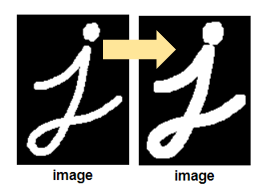
\includegraphics{dilation}
    \caption{แสดงการทำการขยายภาพ (Dilation) เพื่อเพิ่มพื้นที่สีขาว}\label{fig:Dilation}
\end{figure}

Erosion คือการกร่อนภาพ หรือก็คือจะลดพื้นที่สีขาวของภาพออกไปซึ่งวิธีการนี้ส่วนใหญ่จะใช้สำหรับการแยกสิ่งที่ของที่อยู่ติดกัน หรือลบ pepper noise ที่เป็น noise เล็กๆได้ โดยจะใช้หลักการเดียวกับการขยายภาพ  (Dilation) เพียงแต่จะเปลี่ยนจากพื้นที่สีขาวให้กลายเป็นพื้นที่สีดำดังรูป

\begin{figure}[H]
    \centering
    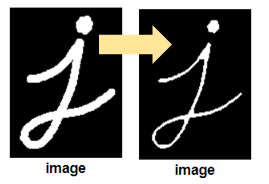
\includegraphics{erosion}
    \caption{แสดงการทำกร่อนภาพ (Erosion) เพื่อกร่อนพื้นที่สีขาว}\label{fig:Erosion}
\end{figure}

\subsection{Optical Character Recognition (OCR)}

OCR เป็นกระบวนการของการแปลงอักษรบนสื่อสิ่งพิมพ์ให้เป็นข้อความที่สามารถค้นหา เปลี่ยนแปลงและแก้ไขได้โดยที่ไม่ต้องพิมพ์ขึ้นมาใหม่ ด้วยการทำ Deep learning ในการเรียนรู้ภาพเพื่อแปลงออกมาเป็นตัวอักษร ซึ่งในโปรเจคของทางผู้จัดทำต้องทำระบบเกี่ยวกับค้นหาที่จะต้องคัดคำออกมาจากสิ่งพิมพ์เหล่านั้น จึงจำเป็นที่จะต้องใช้ OCR ในการแปลงภาพต้นแบบออกมาให้เป็นตัวอักษรก่อนที่จะนำไปใช้งานต่อ

จากการศึกษาพบว่าการทำ OCR ภาษาไทยนั้นมีอยู่มากมายในปัจจุบัน หนึ่งในนั้นมี T - OCR ซึ่งเป็น Library ของ AI For Thai \cite{nectec} และ Tesseract ของ Google \cite{google} ที่ใช้สำหรับแปลงภาพเป็นตัวอักษร โดยกลุ่มของเราเลือกที่จะใช้ Tesseract ในการทำ OCR เนื่องจากไม่เสียค่าใช้จ่ายเมื่อเทียบกับการใช้ OCR ของ AI For Thai นอกจากนั้นเรื่องของการเรียกใช้งานอย่างต่อเนื่อง Tesseract สามารถทำได้ดีกว่าเนื่องจากไม่จำเป็นต้องเรียกใช้งาน AI For Thai จากภายนอก

\subsection{Natural language processing}

Natural language processing คือกระบวนการที่ใช้ในทางปัญญาประดิษฐ์ซึ่ง เป็นกระบวนการที่ทำการวิเคราะห์ทางด้านภาษาซึ่งเอาไปประยุกต์ทำให้ปัญญาประดิษฐ์ (AI) สามารถทำให้คอมพิวเตอร์เข้าใจภาษาและตอบกลับได้ใกล้เคียงกับมนุษย์มากขึ้น โดยในโปรเจคนี้จะใช้มาช่วยในการหาคำสำคัญของหนังสือ และบทความต่าง ๆ เพื่อช่วยให้การค้นหาบทความมีประสิทธิภาพมากขึ้น

\subsubsection{Information retrieval}

Information retrieval คือ เทคโนโลยีการเก็บข้อมูลอย่างนึงโดยจะมีทั้งหมด 2 ลักษณะ ลักษณะที่ 1 คือ Boolean Retrieval เป็นการสร้างโครงสร้างข้อมูลในรูปแบบ Matrix ที่มีค่าเพียงแค่ 0,1 โดยที่ 0 คือไม่มีคำ (Term) ในหนังสือนั้น และ 1 คือมีคำ (Term) อยู่ภายในหนังสือนั้นหรือเรียกได้ว่าเป็น Term-Document Incidence  Matrix ดัง ตารางที่ 2.1 โดยที่ถ้าเราพิจารณาในรูปแบบแถวเราจะได้ Vector ของ Term นั้นที่ปรากฏอยู่ในหนังสือ ไหนบ้าง แต่การเก็บในรูปแบบ Boolean Retrieval เมื่อมีหนังสือ เยอะขึ้นจะทำให้เกิดค่า 0 ที่ไม่มีประโยชน์มากขึ้นจึงมีลักษณะที่ 2 คือโครงสร้างแบบ Inverted index เป็นการเก็บเพียง Term นั้นอยู่ภายในหนังสือ ไหนบ้างเพื่อจะเก็บแต่เพียงข้อมูลสำคัญเอาไว้ดัง ตารางที่ 2.2 โดย คำ (Term) จะผ่านกระบวนการเตรียมข้อมูลตัวอักษร ประกอบไปด้วย Tokenization (การตัดคำจากประโยชน์), Normalization (การจัดการคำย่อ), Stemming (การแปลงคำให้อยู่รูปแบบเดียวกัน), Stop words (จัดการคำที่ไม่มีความหมาย) เพื่อเป็นการจัดรูปของคำให้อยู่ในรูปแบบเดียวกันก่อนที่จะนำไปใช้งาน ซึ่งการเก็บข้อมูลแบบ Information retrieval (IR) จะทำให้การค้นหาข้อมูลภายในฐานข้อมูลได้อย่างรวดเร็วและมีประสิทธิ์ภาพ
\begin{table}[H]
\caption{Information retrieval ในลักษณะ Boolean Retrieval}\label{tbl:ir}
    \begin{tabular}{|l|c|c|c|c|c|}
        \hline
                  & Antony \& Cleopatra & Julius Ceasar & The Tempest & Hamlet & Othello \\ \hline
        Antony    & 1                   & 1             & 0           & 0      & 0       \\ \hline
        Brutus    & 1                   & 1             & 0           & 1      & 0       \\ \hline
        Ceasar    & 1                   & 1             & 0           & 1      & 1       \\ \hline
        Calpurnia & 0                   & 0             & 1           & 0      & 0       \\ \hline
        Cleopatra & 1                   & 0             & 1           & 1      & 1       \\ \hline
        Mercy     & 1                   & 0             & 1           & 1      & 1       \\ \hline
        \end{tabular}
\end{table}

    \begin{figure}[H]
        \centering
        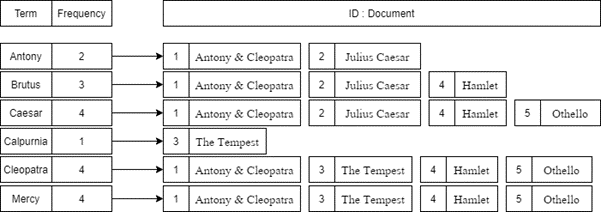
\includegraphics{ir}
        \caption{Information retrieval ในลักษณะ Index Retrieval}\label{fig:ir}
    \end{figure}

\subsubsection{TF-IDF}

เป็นเทคนิคในการคัดแยกคำตามความสำคัญผ่านการให้น้ำหนักในแต่ละคำ โดยแบ่งเป็นสองส่วนนั้นก็คือ TF (Team Frequency) เป็นการดูว่าคำนี้ หรือว่า Term นี้ปรากฏขึ้นภายใน document มากน้อยเพียงไหน และ IDF (Inverse  Document Frequency) คือการหาความผกผันในความถี่ของหนังสือโดยคะแนนความผกผันที่ทำให้รู้ว่าคำนี้เป็นคำที่มีความสำคัญเฉพาะภายในหนังสือนี้ แต่เนื่องจากการดูคะแนน IDF เพียงอย่างเดียวไม่สามารถบอกได้ว่า Term นั้นเป็นคำสำคัญ จึงจำเป็นต้องนำค่า TF มาคูณกับ IDF เป็นค่า TF-IDF เพื่อดูความสำคัญของ Term นั้น ในส่วนการคำนวณนี้เพื่อนำไปใช้ในการค้นหาแบบ Cosine Similarity ต่อไป โดยที่ TF จะใช้เป็น Log normalization โดยคำนวณได้จากสมการ 2.1 ซึ่ง $f_{t,d}$ คือความถี่ของคำ (Term) ที่ปรากฏขึ้นภายใน Document ส่วน IDF จะคำนวณจากสมการ 2.2 ซึ่ง N คือจำนวน Document ที่มีภายในระบบ และ $n_{t}$ คือ จำนวนของ document ที่มีคำ (term) นี้อยู่ เมื่อหาค่าทั้ง TF และ IDF ได้แล้วก็จะหาค่าของ TF-IDF ได้จากสมการ 2.3

\begin{equation}
    tf=\log{(1+f_{t,d})}
    \end{equation}

\begin{equation}
    idf=\log{\frac{N}{n_{t}}}
\end{equation}

\begin{equation}
    TF-IDF=tf*idf
    \end{equation}    

\subsubsection{Cosine Similarity}

เป็นหน่วยวัดความคล้ายคลึงกันระหว่างข้อมูลสอง Vector โดยวัดจากมุม cosine ของจาก Vector ทั้งสองโดยคำนวณได้จากสมการ 2.4 โดยที่ ||x||,||y|| คือ สมการของ Euclidean norm ของ Vertor x, y ดังสมการ 2.5 โดยในโปรเจคนี้เราได้นำค่าน้ำหนักของ TF-IDF มาเป็นน้ำหนักในการคิดค่า Cosine Similarity โดยนำประโยคที่จะค้นหามาผ่านกระบวนการเตรียมข้อมูลตัวอักษร ก่อนที่จะนำมาค้นหาว่า document ไหนมีค่า relevance score (คะแนนความสัมพันธ์) เพื่อนำมาเรียงค่าคะแนนสูงสุดแสดงเป็นผลลัพธ์การค้นหา


\begin{equation}
    \sin(x,y)=\frac{x*y}{\|x\|\|y\|}
\end{equation}    

\begin{equation}
    \|x\|=\sqrt{x_{1}^2+x_{2}^2+\cdots+x_{n}^2}
\end{equation}    
\subsubsection{Minimum Edit Distance}

เป็นหลักการที่หาระยะห่างที่สั้นที่สุดจากคำนึงไปสู่อีกคำนึงจะมีความแตกต่างกันเท่าไหร่ซึ่งจะหลักการเช็คความห่างของคำทั้งหมดสามรูปแบบ
\begin{itemize}
    \item รูปแบบ Insert(I) จะเป็นการเพิ่มตัวอักษรลงไปในคำนั้น เพื่อคำดั้งเดิมของเราจะเปลี่ยนแปลงเป็นคำที่เราต้องการ
    \item รูปแบบ Delete(D) จะเป็นการลบตัวอักษรออกไปในคำนั้น เพื่อคำดั้งเดิมของเราจะเปลี่ยนแปลงเป็นคำที่เราต้องการ
    \item รูปแบบ Replace(R) จะเป็นการเปลี่ยนตัวอักษรนั้นให้เป็นตัวอักษรใหม่ เพื่อคำดั้งเดิมของเราจะเปลี่ยนแปลงเป็นคำที่เราต้องการ
\end{itemize}
\begin{figure}[H]
    \centering
    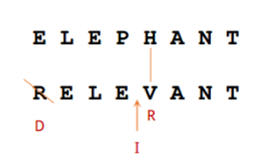
\includegraphics{editdistance}
    \caption{หลักการการเช็ค edit distance \cite{ritambhara}}\label{fig:editdistance}
\end{figure}
หลังจากมีรูปแบบการวัดระยะห่างของคำดังรูปภาพที่ \ref{fig:editdistance} แล้ว จะต้องทำการหาคำที่สั้นที่สุดผ่านรูปแบบของตารางดังรูปภาพที่ \ref{fig:minimumtable} ซึ่งการคำนวณผ่านตารางจะเป็นการนำการกระทำก่อนหน้ามาคำนวนเรื่อย ๆ จนได้รูปการเปลี่ยนเป็นคำใหม่ที่ใช้การเปลี่ยนน้อยที่สุด
\begin{figure}[H]
    \centering
    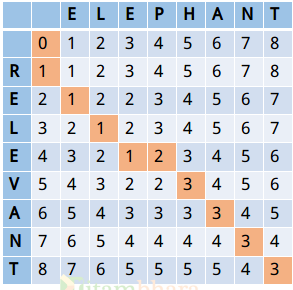
\includegraphics{minimumtable}
    \caption{ตัวอย่างตารางการทำ Minimum edit distance \cite{ritambhara}}\label{fig:minimumtable}
\end{figure}

ซึ่งในโปรเจคของเราได้ดึงหลักการ Minimum edit distance มาใช้ในการตรวจสอบหาคำที่สะกดไม่ถูกต้องโดยมีเกณฑ์ตั้งไว้ว่าถ้าเกินที่กำหนดไว้จะถือว่าคำ ๆ นั้นสะกดไม่ถูกต้องแล้วถูกแก้ให้เป็นคำที่สะกดถูกต้อง

\subsubsection{Spelling Corrector by Peter Norvig}

หลักการการแก้คำผิดของ Peter Norvig\cite{norvig} เป็นการนำคำที่ถูกพิมพ์เข้ามาสร้างมาเป็นคำใหม่โดยการแบ่งคำ การลบคำ การกลับคำ การแทนที่คำ การเพิ่มคำ 
และนำคำที่สร้างใหม่ไปเช็คในพจนานุกรมภาษาว่ามีคำที่สร้างใหม่คำนั้นหรือไม่ ถ้ามีให้นำคำที่ได้ไปหาค่าความน่าจะเป็นของคำที่มีโอกาสเกิดขึ้นมากที่สุด ซึ่งใน Library 
นี้ Norvig ได้นำไปหาโดยใช้ข้อมูลจาก Corpus ที่สร้างขึ้นจากคำที่ได้จาก Project Gutenberg\cite{guten}, Wikitionary\cite{wikitionary} และ British 
National Corpus\cite{kilgarriff} ที่จะรวมคำต่างเอาไว้ จากนั้นคำนวนความน่าจะเป็นของคำที่เกิดขึ้นโดยใส่คำที่ต้องการหาแล้วนับว่าใน Corpus นั้นมีคำนั้นปรากฏขึ้นเท่าไร
หารด้วยจำนวนคำของ Corpus ทั้งหมด ก็จะได้ความน่าจะเป็นออกมา ซึ่งคำที่จะแก้ก็จะเลือกจากคำที่มีค่าความน่าจะเป็นมากที่สุด โดย library PyThaiNLP\cite{pythainlp} และ Pyspellchecker\cite{pypi} 
นั้นก็ใช้หลักการเดียวกันกับการแก้คำผิดของ Peter Norvig 

\subsection{RESTful Service}
เป็นการสร้าง web service โดยเรียกใช้ผ่านทาง HTTP Method ทั้ง 4 ประเภท GET/POST/PUT/DELETE ส่งข้อมูลออกมาเป็นรูปของ XML ทำให้ปริมาณข้อมูลที่ส่งมาน้อยกว่าการใช้ Protocol SOAP  โดยโครงสร้างของ 
HTTP Request ดังรูปภาพที่ \ref{fig:httpreq} ประกอบด้วย 

\begin{enumerate}
 \item VERB: แสดง method ของ HTTP
 \item URI: ตำแหน่งของข้อมูลที่ต้องการ
 \item HTTP Version: เวอร์ชั่นของ HTTP
 \item Request Header: Metadata ที่เก็บข้อมูลในรูปแบบ Key-Value ของ header
 \item Request Body: ส่วนเก็บข้อมูลของเนื้อหา
\end{enumerate}

\begin{figure}[H]
    \centering
    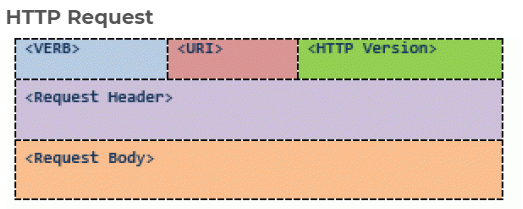
\includegraphics{httpreq}
    \caption{แสดงถึงโครงสร้างของ HTTP Request \cite{Saixiii}}\label{fig:httpreq}
\end{figure}

HTTP Response ดังรูปภาพที่ \ref{fig:httpres} ประกอบด้วย


\begin{enumerate}
	\item HTTP Version: เวอร์ชั่นของ HTTP
	\item Response Code: รหัสผลลัพธ์ของการทำงานในระดับ HTTP เป็นเลข 3 หลัก
	\item Response Header: Metadata ที่เก็บข้อมูลในรูปแบบ Key-Value ของ header
	\item Response Body: ส่วนเก็บข้อมูลของเนื้อหา

   \end{enumerate}
   
\begin{figure}[H]
    \centering
    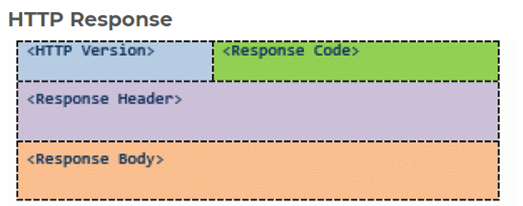
\includegraphics{httpres}
    \caption{แสดงถึงโครงสร้างของ HTTP Response \cite{Saixiii}}\label{fig:httpres}
\end{figure}

\subsection{Word Embedding}

เป็นวิธีการที่จะเปลี่ยนคำปกติเป็น vector ที่อยู่ในหลากหลายมิติและขนาดเพื่อให้สามารถเปรียบเทียบคำต่าง ๆ ว่ามีความสัมพันธ์ใกล้เคียงกับคำไหนบ้างในระบบเพื่อ
ที่ใช้สำหรับการหาคำที่มีความหมายใกล้เคียงกันโดยมีการทำ word embedding มากมายไม่ว่าจะเป็น Word2Vec \cite{xin} \cite{Goldberg} ที่ถูกสร้างโดยทีมวิจัยของ 
Google FastText \cite{fasttext} เป็น word embedding อีกหนึ่งตัวที่สร้างขึ้นจากทีมวิจัยของ facebook หรือจะเป็น ELMo \cite{matthew} ที่เป็นรูปแบบการ word embedding ที่ดูรูปคำโดยรอบเป็นต้น 

\subsubsection{Word2Vec}
ทฤษฎี Word2Vec\cite{shortStoryForWord2Vec} เป็นทฤษฎีที่ช่วยจัดการกับคำศัพท์ที่มีความหมายใกล้เคียงกัน หรือคำศัพท์ที่มีความสัมพันธ์อย่างคำตรงข้ามกัน 
อย่างคำว่า พระราชา กับ กษัตริย์ ที่เป็นคำที่ความหมายใกล้เคียงกัน แต่ตรงข้ามกับคำว่า ราชินี โดยทั้งหมดนี้จะถูกจัดเก็บในรูปแบบของเวกเตอร์
แน่นอนว่าการที่จะรู้ว่าแต่ละคำมีความสัมพันธ์ได้นั้น เราจำเป็นต้องสร้างประเภทของคำจากรูปประโยคอย่างเช่น “การ เลี้ยง หมา เป็น สัตว์เลี้ยง ถือ เป็น การ ผ่อนคลาย” 
กับ “แมว ถือ เป็น สัตว์เลี้ยง ที่ สุขุม” จากทั้งสองประโยคจะเห็นว่าคำที่เหมือนกันจากทั้งสองประโยค จะเป็นคำว่า สัตว์เลี้ยง ซึ่งการทำ Word2Vec 
จะเป็นการดึงประเภทโดยเช็คจากคำใกล้เคียงเพื่อจัดกลุ่ม ดังนั้นจากคำว่า สัตว์เลี้ยง ที่มีคำว่า หมา และ แมว เป็นสัตว์เลี้ยงเช่นเดียวกัน จะแสดงว่าคำว่า 
หมา และ แมว มีความหมายใกล้เคียงกันจากความสัมพันธ์กัน ทั้งนี้การที่แต่ละคำจะมีสัมพันธ์ที่เชื่อมโยงกันได้มาก หรือน้อยขึ้นอยู่ระยะของคำ (Window Size) 
ยกตัวอย่างถ้ามีค่ามาก คำว่าสัตว์เลี้ยงอาจจะมีคำที่ไม่เกี่ยวข้องเกิดขึ้นหากข้อมูลไม่เพียงพอ เช่น ตู้เย็น หมา แมว เป็นสัตว์เลี้ยง แต่ถ้าหากค่าน้อยเกินไป หมา 
อาจจะไม่ถูกนับเป็นประเภทสัตว์เลี้ยงแทน
นอกจากส่วนการใช้คำข้างเคียงมาช่วยในการทำ Word2Vec แล้วยังมีส่วนของรูปแบบการสร้างโมเดลเพื่อหาคำที่มีความสัมพันธ์กันอีกด้วย 
โดยจะมีสองรูปแบบคือ CBOW (continuous bag of words) จะเป็นรูปแบบของการที่ใช้คำหลาย ๆ คำเผื่อมาหาคำเพียงคำเดียว 
และ Skip-Gram ที่จะตรงข้ามกับรูปแบบที่แล้วคือ การที่ใช้คำหนึ่งคำเพื่อหาคำหลายคำออกมา

\begin{figure}[H]
    \centering
    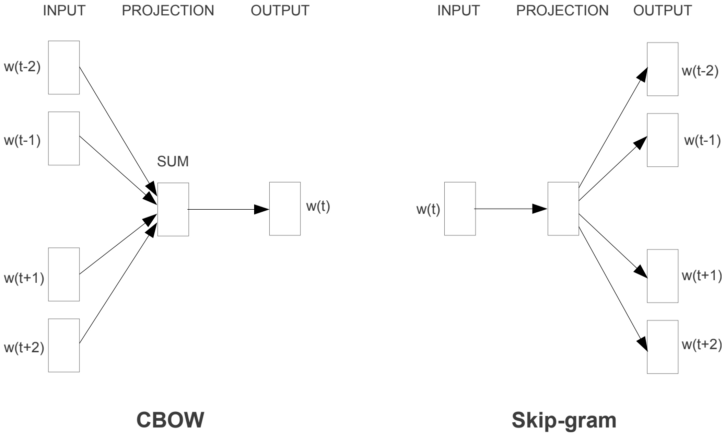
\includegraphics[scale=0.5]{cbowskip}
    \caption{ภาพแสดงโมเดล Skip-gram และ CBOW \cite{ichi}}\label{fig:cbowskip}
\end{figure}

\subsubsection{Skip-gram}

Skip-gram\cite{ichi} เป็นโมเดลที่จะใช้หาความสัมพันธ์ของคำ โดยจะนำคำที่เข้าไปไปหาคำบริบทโดยรอบ โดยการที่โมเดลจะทำการอ่านประโยคเข้าไปและเรียนรู้จากประโยค 
โดยการพิจารณาบริบทโดยรอบของคำ อย่างเช่น Thou shalt not make a machine in the likeness of human a mind โมเดลก็จะทำการรับคำ 
1 คำเข้าไปและพิจารณาคำรอบๆ เริ่มจากว่า not ก็จะพิจารณาสองคำก่อนหน้าและสองคำหลัง (ตามจำนวน window size ในที่นี้กำหนด window size เป็น 2) 
ซึ่งจะได้มา 4 คำ คือ Thou, shalt, make และ a ดังรูปที่ \ref{fig:skipgram} ซึ่งโมเดลก็จะทำการเรียนรู้คำไปเรื่อยๆเพื่อ weight น้ำหนักภายในโมเดล
\begin{figure}[H]
    \centering
    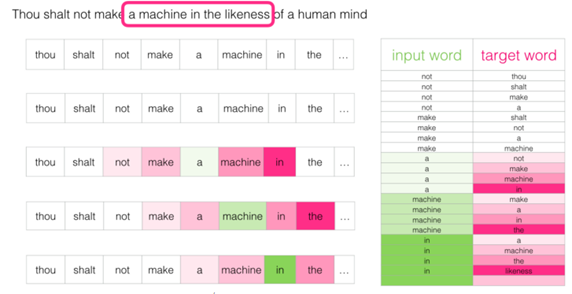
\includegraphics{skipgram}
    \caption{แสดงการทำงานของ Skip-gram \cite{ichi}}\label{fig:skipgram}
\end{figure}

\subsubsection{CBOW}
CBOW\cite{ichi} เป็นโมเดลที่จะใช้หาความสัมพันธ์ของคำแบบจะพิจารณาคำหลายๆคำเพื่อหาคำหนึ่งคำ ดังตัวอย่างในรูปที่ \ref{fig:cbow} โดยการที่โมเดล
จะทำการอ่านประโยคเข้าไปและเรียนรู้จากประโยคเหมือนโมเดล Skip-gram อย่างเช่น Thou shalt not make a machine in the likeness of human a mind 
โมเดลก็จะทำการอ่านคำตามจำนวน window size ถ้า window size เป็น 2 ก็จะเป็นการกำหนดว่าอ่าน input เข้าไป 2 คำและคำถัดจาก 2 คำนั้นในประโยคจะเป็น
ผลลัพธ์ที่ได้จาก input  อย่างเช่นถ้าใส่ thou,shalt เข้าไปก็จะได้คำว่า not ออกมา ซึ่งจะสร้างโมเดลนี้ก็จะต้องใส่ข้อมูลประโยคจำนวนมากเพื่อทำการ weight 
ค่าน้ำหนักภายในโมเดล ให้มีประสิทธิภาพคล้ายกับโมเดล skip-gram

\begin{figure}[H]
    \centering
    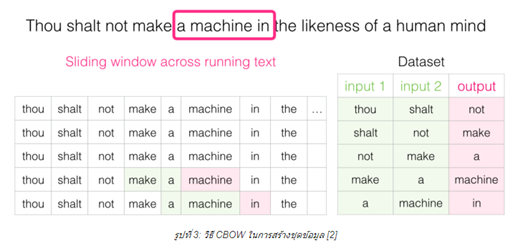
\includegraphics{cbow}
    \caption{แสดงการทำงานของ CBOW \cite{ichi}}\label{fig:cbow}
\end{figure}

\section{ภาษาคอมพิวเตอร์และเทคโนโลยี }

\subsection{Open source Computer Vision (OpenCV)}

เป็นซอฟต์แวร์ที่เกี่ยวกับการประมวลผลภาพที่มีการสนับสนุนการพัฒนามาจาก Intel Corporation โดยที่ตัว OpenCV นั้นเป็น Library Open Source  โดยมีจุดประสงค์เพื่อให้นำไปต่อยอดการพัฒนาโปรแกรมในด้าน การรับรู้มองเห็นของคอมพิวเตอร์ (Computer Vision) ให้เข้าใจไม่ว่าจะเป็นภาพนิ่ง (Image) หรือจะเป็นภาพเคลื่อนไหว (Video) โดยภายในโปรเจคนี้ได้นำ OpenCV มาเป็นตัวทำการเตรียมข้อมูลรูปภาพ โดยที่นำรูปภาพที่ได้มาจากสแกนหนังสือ / หนังสือ มาทำการปรับปรุงคุณภาพรูปภาพให้เหมาะสมกับการทำส่วน Optical Character Recognition (OCR) ให้มีความแม่นยำมากยิ่งขึ้นเช่นการลบรูปภาพ การลบสิ่งที่ลบกวน การลบกรอบตาราง การหมุนรูป 

\subsection{Tesseract OCR}

เป็นหนึ่งใน Library ที่เกี่ยวกับการทำ Optical Character Recognition (OCR) ที่ถูกพัฒนาโดย Google โดยเป็น Library Open Source ที่ใช้ในการทำเกี่ยวกับ Text Detection โดยสามารถเรียกใช้งานได้ผ่าน Command line หรือจะเป็นการเรียก API ภายในโปรเกรมก็ทำได้นอกจากนั้น Tesseract เวอร์ชั่น 5.0.0 beta มีการใช้ Convolutional Neural Network (CNN) \cite{keiron} ร่วมกันกับ Long Short-Term Memory (LSTM) เพื่อให้การทำนายผลได้ดีขึ้นโดยเราจะนำตัว Tesseract มาทำเป็น OCR ภายในโปรเจคนี้

\subsection{DeepCut}

เป็น Library ในภาษา Python ที่สร้างมาจาก True Corporation โดยมีลักษณะเด่นที่ใช้ CNN (Convolutional Neural network) \cite{keiron} มาช่วยทำให้ผลลัพธ์ที่ได้ออกมามีความแม่นยำที่ค่อนข้างสูง  ซึ่งโปรเจคของเราต้องการ DeepCut เพื่อที่จะสามารถไปตัดคำจากรูปประโยคภาษาไทยที่มีความซับซ้อน และไม่แบ่งแยกชัดเจนเหมือนภาษาอังกฤษ 

\subsection{ReactJS}

เป็นหนึ่งใน Library หรือจะเรียกว่าเป็น Framework ที่ Facebook  เป็นคนสร้างขึ้นโดยที่มีหน้าที่เป็นการสร้าง UI โดยมีความคิดมากจากรูปแบบ MVC \cite{techterms} (Model View Controller) หรือก็คือเป็นตัวจัดการกับ Model กับ View ของตัวเว็บไซต์ โดยในโปรเจคนี้ได้เลือกใช้ ReactJS เป็น Front End สำหรับการทำ platform Web Application 

\subsection{Python}

Python เป็นภาษาทางโปรแกรมมิ่งซึ่งเป็นภาษาทางคอมพิวเตอร์ระดับสูงที่ออกแบบมาให้ใกล้เคียงกับภาษามนุษย์มากที่สุดเพื่อให้สามารถเข้าใจได้ง่ายมากขึ้น ซึ่งในโปรเจคมีข้อมูลที่ต้องประมวลในแต่ละครั้งมีขนาดใหญ่อาจจะทำให้เกิดความล่าช้าในแต่ละการประมวล ทางผู้จัดทำจึงเลือกใช้ Python เนื่องจากรองรับในส่วนของการทำ Thread รวมถึงนำมาใช้ในการทำ Data preparation ทั้งการเตรียมข้อมูลรูปภาพ และการเตรียมข้อมูลต่างๆหลังจากการทำ OCR นอกจากนี้ยังใช้ในการทำ Web Server อีกด้วย 

\subsubsection{Django}

เป็น REST Framework ที่ใช้ภาษา Python เป็นฐาน โดยในโปรเจคนี้เราจะนำมาสร้าง REST API  เพื่อใช้ในการใช้ Library อย่างเช่น DeepCut หรือ OCR ที่สามารถใช้ร่วมการแบ่ง Multi Thread ได้อย่างมีประสิทธิภาพ และยังสามาถจัดการข้อมูลใน database สำหรับโปรเจคนี้

\subsection{NodeJS}

NodeJS เป็นเสมือนแพลตฟอร์มที่ใช้ภาษา JavaScript ที่มี Library สำหรับใช้จัดการกับฝั่ง Server ซึ่ง NodeJS นั้นมีความยืดหยุ่นสูงที่สำหรับการจัดการ Web Server โดย Library ที่นำมาใช้คือ Express เป็น Web Server ที่เป็น RESTful API ได้
\chapter{การออกแบบและระเบียบวิธีวิจัย}

\section{ภาพรวมของระบบ}

บทนี้จะกล่าวถึงภาพรวมของระบบโดยแสดงเป็นไดอะแกรมดังรูปที่ \ref{fig:systemoverview} ซึ่งประกอบไปด้วยการออกแบบระบบฐานข้อมูล ระบบการตัดคำ ระบบการประมวลรูปภาพ และการออกแบบ User Interface สำหรับการใช้งาน

\begin{figure}[H]
    \centering
    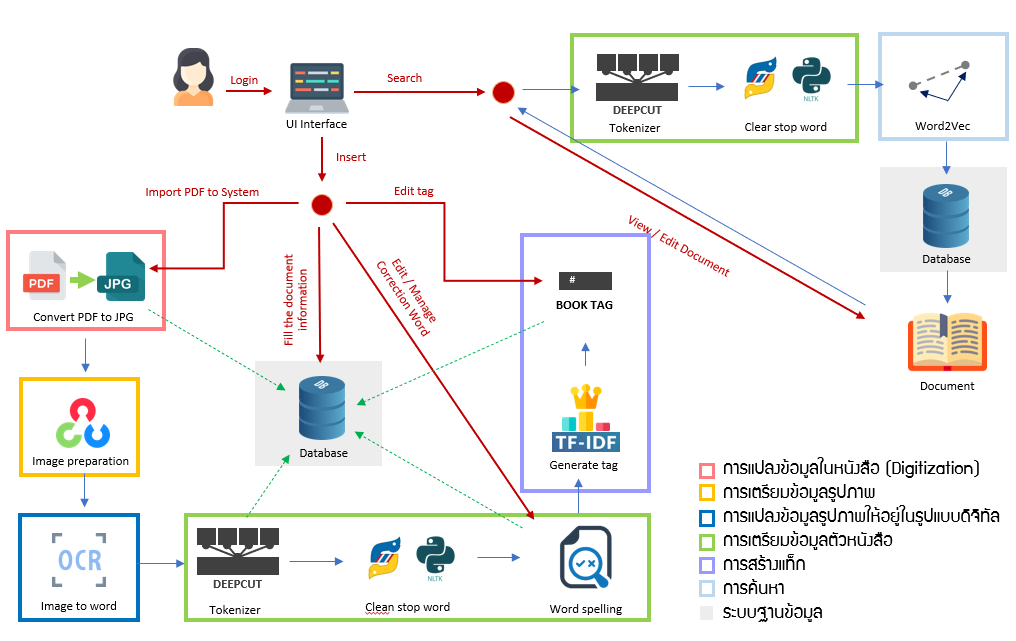
\includegraphics[scale=0.5]{systemoverview}
    \caption{ภาพรวมของระบบ}\label{fig:systemoverview}
\end{figure}

\section{การออกแบบการทดลอง}
\subsection{การแปลงข้อมูลในหนังสือ (Digitization) }

สำหรับการแปลงข้อมูลในหนังสือ (Digitization) ผู้ใช้จะต้องทำการอัปโหลดไฟล์ PDF ของหนังสือเข้าสู่ระบบหลังจากนั้นจะระบบจะทำการแปลงแต่ละหน้าเป็นรูปภาพ JPG เพื่อนำไปใช้ต่อในขั้นต่อไปและนำใช้แสดงภายใน web application

\subsection{การเตรียมข้อมูลรูปภาพ}

ในส่วนของการจัดการรูปก่อนที่จะทำการ OCR ซึ่งรูปภาพนำมา OCR นั้นมาจากการสแกนทำให้ภาพส่วนใหญ่อยู่ในสภาพดีแต่ก็ยังคงมี noise  และมีความผิดพลาดจากการสแกนเช่น ภาพเอียง
 หรือตัวอักษรไม่ชัดเกิดจากการขยับในระหว่างการสแกน หรือมีพื้นหลังสีที่ทำให้ OCR ไม่มีประสิทธิภาพ ดังนั้นจึงต้องมีการเตรียมข้อมูลรูปภาพก่อนที่จะไปทำ OCR
ซึ่งในการเตรียมข้อมูลรูปภาพ นั้นทางคณะผู้จัดทำได้ออกแบบไว้ว่าจะทำการแยกระหว่างรูปและตัวอักษรออกจากกัน โดยการใช้คอนทัว (Contour) เข้ามาช่วยในการคัดแยกรูปออกจากตัวอักษร 
โดยดูจากพื้นที่สี่เหลี่ยมที่ของคอนทัว (Contour) กับพื้นที่คอนทัว (Contour) ว่ามีความต่างขนาดและความแตกต่างกันมากเท่าไร หรือใช้ขนาดความกว้างและยาวมาดูว่ามีขนาดเกินเท่าไรถึงจะตัดให้เป็นรูปภาพ
นอกจากนี้ออกแบบการหมุนโดยสร้างคอนทัว (Contour) บรรทัดและวัดความเอียงของแต่ละบรรทัดว่าเอียงเท่าไรจากนั้นจึงหมุนกลับในองศาตรงข้าม


\subsubsection{การคัดเลือกข้อมูล}
เนื่องจากข้อมูลหนังสือที่ทางคณะผู้จัดทำนำมาใช้นั้นมีความหลากหลาย และบางเล่มมีหน้าหนังสือพื้นหลังสีที่ส่งผลให้การทำ OCR ได้ผลลัพธ์ที่ไม่ดีดั้งนั้นจึงทำการคัดเลือกข้อมูลหนังสือเพื่อลดโอกาสที่จะเกิดคำผิดที่จะเกิดขึ้น 
โดยการทำการคัดเลือกข้อมูลที่เป็นหน้าสีนั้น เราได้นำค่าความถี่ของหน้าที่มีพื้นหลังสีมาพล็อตเพื่อหาความแตกต่างจะเห็นได้ว่าถ้าหน้าที่มีพื้นหลังสี หลายสีนั้นจะมีค่าความถี่กระจายอยู่หลายค่าในขณะที่ถ้าเป็นหน้าที่มีพื้นหลัง
สีเดียวมีค่าความถี่ในช่วงนั้นสูงดังรูป \ref{fig:skippage}

\begin{figure}[H]
    \centering
    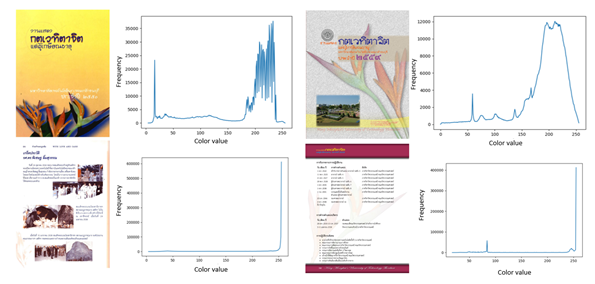
\includegraphics[scale=0.8]{skippage2}
    \caption{ภาพแสดงความถี่ของภาพพื้นหลังสีและภาพพื้นหลังขาวดำ}\label{fig:skippage2}
\end{figure}

\underline{ขั้นตอนหลักการทำงานของการคัดเลือกข้อมูล}

\begin{enumerate}
    \item รับไฟล์รูปภาพมาแปลงเป็น Gray Scale และทำการปรับตัวแปรที่เป็นรูปภาพแบบ Gray Scale ให้เป็นอาเรย์มิติเดียว
    \item ทำการนับความถี่ของค่าสีว่าแต่ละค่าสีนั้นมีจำนวนเท่าไหร่
    \item นำค่าความถี่ของค่าสีที่มีความถี่สูงสุดมาคำนวณว่ามีค่ามากกว่า 10 เปอร์เซ็นต์ของจำนวนพิกเซลทั้งหมดหรือไม่ ถ้าน้อยกว่าให้ข้ามการทำ OCR หน้านี้ไป
\end{enumerate}

\begin{figure}[H]
    \centering
    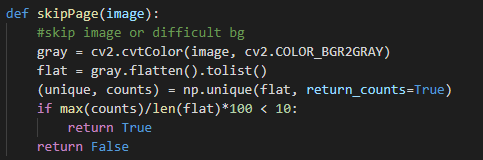
\includegraphics[scale=0.8]{skippage}
    \caption{ภาพแสดงขั้นตอนการคัดเลือกข้อมูล}\label{fig:skippage}
\end{figure}

\subsubsection{การหมุนรูป}
ในส่วนของการหมุนรูปนั้นจัดทำขึ้นมาเพื่อแก้ไขข้อมูลรูปภาพที่เกิดความผิดพลาดจากการสแกนส่งผลให้รูปที่ได้นั้นมีความเอียงและทำให้เกิดความผิดพลาดในการทำ OCR เพื่อข้อมูลภาพให้อยู่ในรูปแบบที่เหมาะสมกับการทำ OCR มากที่สุด
โดยจะมีวิธีการหาค่าองศาของแต่ละประโยคด้วยการนำจุด 2 ที่อยู่ในแนวระราบเดียวกันมาทำการหา Arctan เพื่อหาองศาที่ทำให้บรรทัดนั้นตรง และนำค่าองศาแต่ละบรรทัดที่อยู่ในย่อหน้าเดียวกันมาหาองศาเฉลี่ยเพื่อที่จะใช้การหมุนทั้งย่อหน้าให้ตรง

\underline{ขั้นตอนการหมุน}

\begin{enumerate}
    \item เริ่มจากนำรูปภาพมาทำเป็นสองส่วนคือการทำขยายภาพ (Dilation) และกร่อนภาพ (Erosion) 
    โดยที่รูปภาพที่ถูกขยายจะได้รูปที่มีการจับกลุ่มบรรทัดของย่อหน้า และรูปที่ถูกกร่อนจะได้รูปภาพที่มีการแยกบรรทัดข้อความกันอย่างชัดเจน และนำไปหาคอนทัว 
    (Contour) โดยที่รูปภาพของการจับกลุ่มบรรทัดจะได้ผลลัพธ์ดังรูปภาพที่ \ref{fig:rotate2} ทางด้านซ้าย และการแยกบรรทัดจะได้ผลลัพธ์ดังรูปภาพที่ \ref{fig:rotate2} ทางด้านขวา 
    
    \begin{figure}[H]
        \centering
        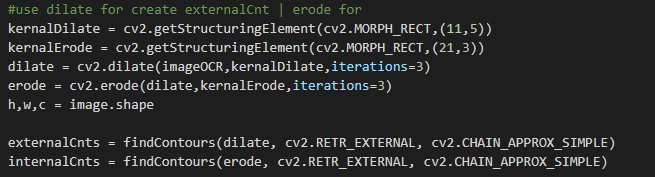
\includegraphics[scale=0.8]{rotate1}
        \caption{ภาพแสดงการทำการกร่อนภาพ (Erosion) และการขยายภาพ (Dilation)}\label{fig:rotate1}
    \end{figure}
    
    \begin{figure}[H]
        \centering
        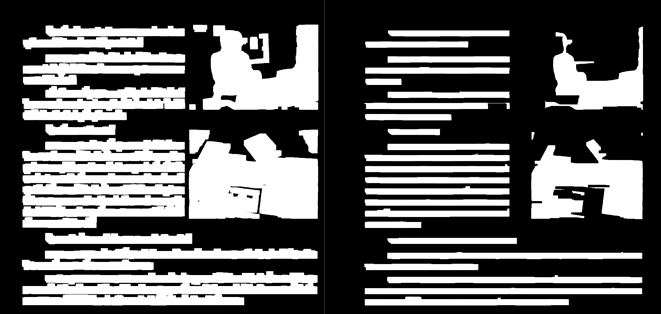
\includegraphics[scale=0.8]{rotate2}
        \caption{ภาพแสดงการเปรียบเทียบการทำการกร่อนภาพ (Erosion) และการขยายภาพ (Dilation)}\label{fig:rotate2}
    \end{figure}

    \item ทำการแยก รูปภาพและบรรทัดข้อความ ภายในคอนทัว (Contour) ที่ถูกกร่อน โดยการกำหนดค่าความสูงสูงที่สุดและต่ำที่สุดไว้ 
    ค่าอัตราส่วนระหว่างความสูงและความกว้าง โดยค่าที่กำหนดไว้เราได้เอามาจากการทำ Page dewarp ของ Matt Zucker \cite{mattzuck} 
    และนำมาตรวจสอบเงื่อนไขและแยกเป็นกลุ่มของข้อความและรูปภาพดังรูปภาพที่ \ref{fig:rotate3}
    
    \begin{figure}[H]
        \centering
        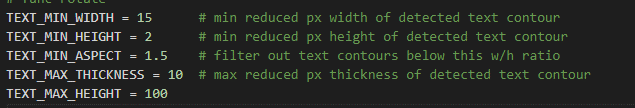
\includegraphics[scale=0.8]{rotate3}
        \caption{ภาพแสดงเกณฑ์การวัดบรรทัดของตัวอักษร}\label{fig:rotate3}
    \end{figure}
    
    \begin{figure}[H]
        \centering
        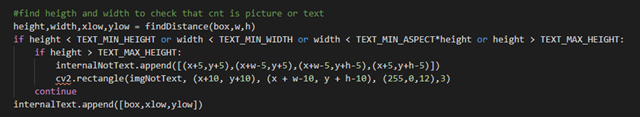
\includegraphics[scale=0.8]{rotate4}
        \caption{ภาพแสดงการคัดแยกคอนทัว (Contour) ที่ไม่ใช่ตัวอักษร}\label{fig:rotate4}
    \end{figure}

    \item ทำการหา Mask เพื่อใช้ในการลบรูปภาพและคำนวณองศาของข้อความแต่ละบรรทัดภายในคอนทัว (Contour) ของภาพที่ถูกขยาย (Dilation) นั้น 
    โดยการลบรูปภาพจะทำโดยการระบุว่ารูปภาพอยู่ภายในคอนทัว (Contour) ไหน เพื่อจะนำมาเป็น mask สำหรับการลบรูปภาพออกด้วยวิธีการดูว่ามุมทั้ง 4 มุมของคอนทัว 
    (Contour) ที่ถูกแยกเป็นรูปภาพนั้นอยู่ภายในคอนทัว (Contour) ภาพที่ถูกขยาย (Dilation) ครบทั้งสี่มุมหรือเปล่า ถ้าใช่แสดงว่าคอนทัว (Contour) ภาพที่ถูกขยาย (Dilation)
     คือ mask ของรูปภาพที่จะต้องถูกลบ ให้สร้างคอนทัว (Contour) ภาพที่ถูกขยาย (Dilation)นั้นลงไปบนรูปแต่ถ้าไม่ใช่ก็จะนำไปหาองศาของแต่บรรทัดข้อความและนำมาเฉลี่ยเป็นองศาที่ต้องหมุนสำหรับคอนทัว 
     (Contour) ภาพที่ถูกขยาย (Dilation) นั้น
    
    \begin{figure}[H]
        \centering
        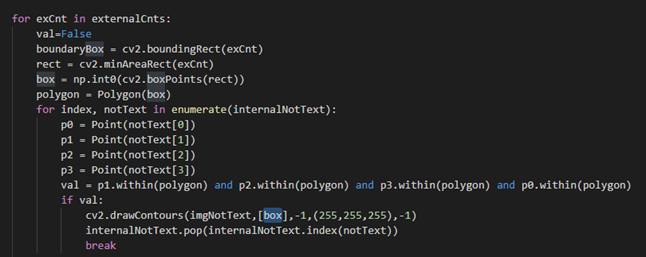
\includegraphics[scale=0.8]{rotate5}
        \caption{ภาพแสดงการทำ Mask ในส่วนที่ไม่ใช่ตัวอักษร}\label{fig:rotate5}
    \end{figure}

    \begin{figure}[H]
        \centering
        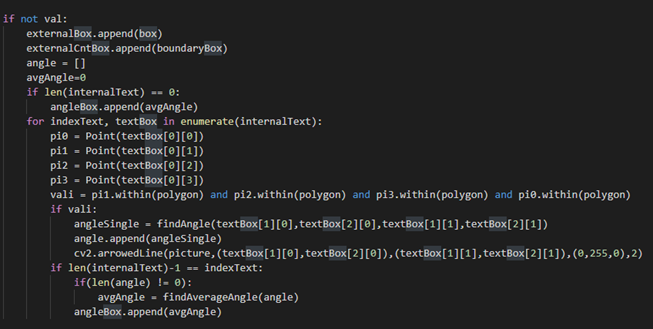
\includegraphics[scale=0.8]{rotate6}
        \caption{ภาพแสดงการคัดตัวอักษรเพื่อนำไปหาองศาในการหมุน}\label{fig:rotate6}
    \end{figure}

    \begin{figure}[H]
        \centering
        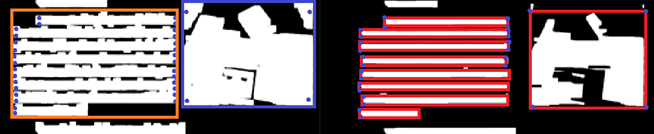
\includegraphics[scale=0.8]{rotate7}
        \caption{ภาพแสดงจุดของคอนทัว (Contour) เล็กในคอนทัว (Contour) ใหญ่}\label{fig:rotate7}
    \end{figure}

    \item นำ Mask ที่เป็นรูปภาพนำมาลบออกโดยเมื่อได้ mask มาก็จะนำไปลบออกจากรูปใหญ่ในฟังก์ชั่น removePicture 
    ในรูปที่ \ref{fig:rotate8}  ซึ่งจะนำเอาคอนทัว (Contour) ภาพที่ถูกขยาย (Dilation) ที่เป็นตัวอักษร (กรอบสีเขียว) 
    มาลบออกจาก mask เดิม(กรอบสีแดง)ที่ได้สร้างไว้เพื่อกันการลบพื้นที่เป็นตัวอักษรดัง \ref{fig:rotate9} ด้วยการใช้ฟังก์ชั่น 
    drawContour ก่อนจะนำ mask ที่ได้มาลบรูปออกทำให้ภาพในแต่ละหน้าหายไป เป็นผลลัพธ์ออกมาดัง \ref{fig:rotate11}
    
    \begin{figure}[H]
        \centering
        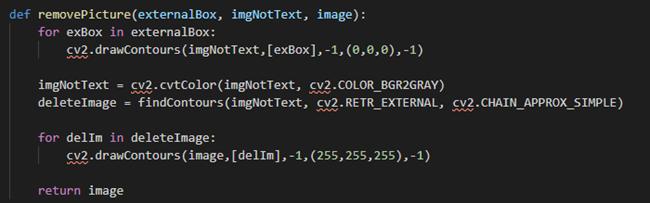
\includegraphics[scale=0.8]{rotate8}
        \caption{ภาพแสดงฟังก์ชั่นการลบรูปภาพออกจากหนังสือ}\label{fig:rotate8}
    \end{figure}

    \begin{figure}[H]
        \centering
        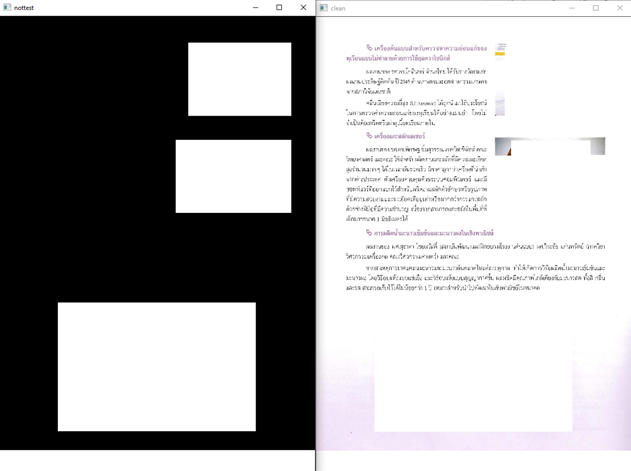
\includegraphics[scale=0.8]{rotate9}
        \caption{ภาพแสดงการสร้าง Mask เพื่อลบรูปภาพ}\label{fig:rotate9}
    \end{figure}

    \begin{figure}[H]
        \centering
        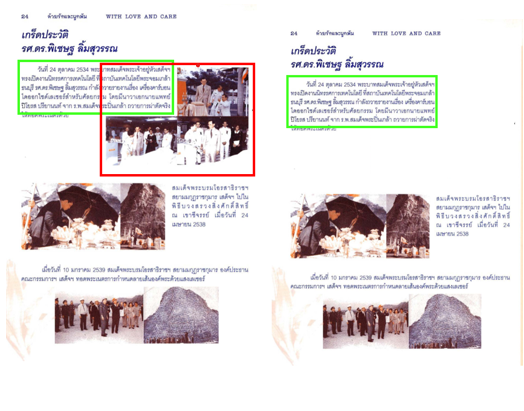
\includegraphics[scale=0.8]{rotate11}
        \caption{ภาพแสดงการสร้าง Mask โดยเว้นที่ตัวอักษร}\label{fig:rotate11}
    \end{figure}

    \item การหาค่าเฉลี่ยองศาในแต่ละรูปภาพที่ถูกขยาย (Dilation) ทำโดยการนำคอนทัว (Contour) 
    ของตัวอักษรแต่ละบรรทัดที่ได้มาเข้าสู่กระบวนการวัดมุมและหมุนภาพ โดยการนำจุดสี่จุดของคอนทัว (Contour) 
    เล็กมาเฉลี่ย องศาในการหมุน เนื่องจากค่าจุดที่ได้จากการหา Minimum Area Rectangle 
    นั้นอาจจะมีบางครั้งที่ค่าจุดที่ส่งมาไม่ได้เริ่มจากซ้ายบน ดังนั้นจุดและเว้นที่หามาได้นั้นอาจจะทำให้ได้องศาในแนวตั้งมาได้ 
    จึงต้องทำการกรองว่าองศาที่ได้ว่าตั้งฉากหรือไม่ตั้งฉากถ้าเป็นองศาตั้งฉากให้หาการเอียงจากแกน 90 องศา 
    แต่ถ้าไม่ใช่ก็เทียบจากแกนแนวนอน 0 องศาหรือ 180 องศา

    \begin{figure}[H]
        \centering
        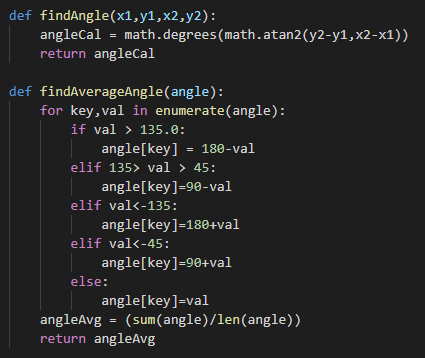
\includegraphics[scale=0.8]{rotate10}
        \caption{ภาพแสดงการหาองศาในการหมุน}\label{fig:rotate10}
    \end{figure}
    
\end{enumerate}

\subsubsection{การลบพื้นหลัง}
ในส่วนของการลบพื้นหลังนั้นเป็นฟังก์ชั่นที่สร้างขึ้นมาเพื่อลบรายละเอียดที่่มีรูปหรือลวดลาย ซึ่งมีผลต่อการแยกแยะและจดจำตัวอักษร 
ซึ่งเป็นฟังก์ชั่นทางเลือกที่ทำขึ้นมาแก้ไขผลลัพธ์ที่ได้จากการจัดการลบรูปภาพ

\underline{ขั้นตอนการลบพื้นหลัง}

\begin{enumerate}
    \item แปลงรูปภาพสีให้กลายเป็นขาวดำจะทำให้ชั้นสีเหลือเพียงชั้นเดียวจากเดิมที่มี 3 ชั้นสีเป็น RGB เหลือเป็นค่า Gray scale ที่มีค่า 0-255 โดยที่ค่าเข้าใกล้ 0 คือสีดำและเข้าใกล้ 255 คือสีขาว
    \item นำรูปภาพมาผ่านกระบวนการขยาย (Dilation) โดยกำหนดเป็นสี่เหลี่ยมขนาด 5x5 จะได้ผลลัพธ์ดังรูปภาพที่ \ref{fig:rem3}
    \item นำรูปภาพ gray scale มาหารกับค่าที่ถูกขยาย (Dilation) มาโดยให้ scale อยู่ที่ 0 – 255 จะทำให้พื้นหลัง หายไปเนื่องจากจะเห็นได้ว่าถ้าส่วนไหนของรูปภาพถูกขยาย (Dilation) ออกไปจะไม่ถูกลบเมื่อนำค่าพิกเซลสี(pixel) นั้นมาหารแต่ถ้าพื้นที่นั้นไม่ถูกขยาย (Dilation) ออกไปจะทำให้เมื่อนำค่าพิกเซลสี(pixel) มาหารจะทำให้พิกเซลสี(pixel) นั้นกลายเป็นสีขาวดังรูปภาพที่ \ref{fig:rem4}
    \item นำรูปภาพที่ไม่มีพื้นหลัง ไปทำ threshold ให้รูปเหลือเพียงสีขาวกับสีดำ โดยเราจะทำเป็น THRESH\_BINARY\_INV ที่ทำให้ตัวอักษรเป็นสีขาวและพื้นหลังเป็นสีดำเพื่อนำไปใช้ในการหาคอนทัว (Contour) ต่อ
    \end{enumerate}

\begin{figure}[H]
    \centering
    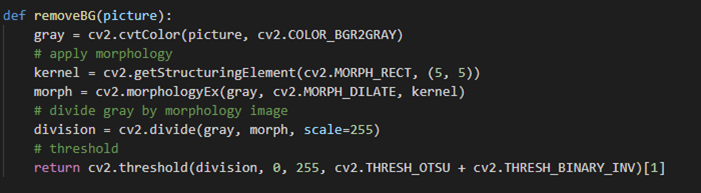
\includegraphics[scale=0.8]{removebg}
    \caption{ภาพแสดงขั้นตอนในการลบพื้นหลังสี}\label{fig:removebg}
\end{figure}

\begin{figure}[H]
    \centering
    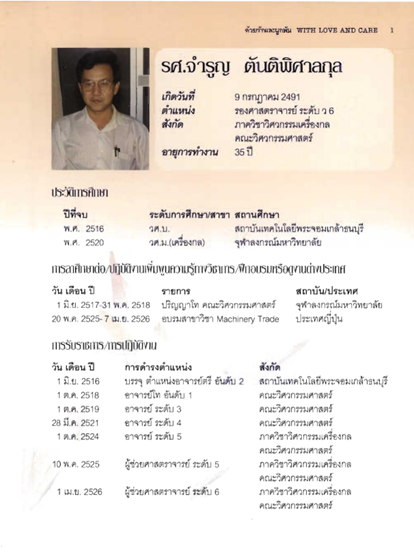
\includegraphics[scale=0.7]{rem1}
    \caption{รูปภาพสีก่อนถูกนำเข้ามาทำการลบพื้นหลัง}\label{fig:rem1}
\end{figure}

\begin{figure}[H]
    \centering
    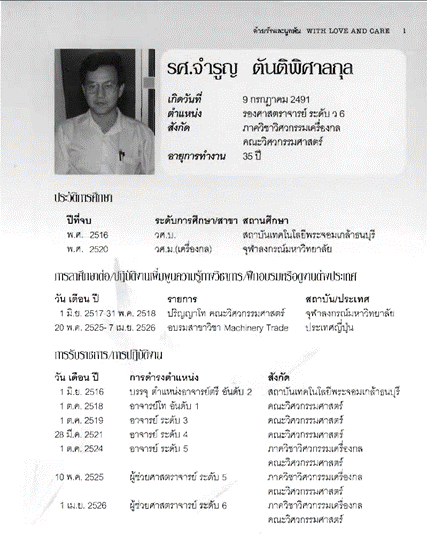
\includegraphics[scale=0.7]{rem2}
    \caption{รูปภาพการแปลงภาพสีเป็น gray scale}\label{fig:rem2}
\end{figure}

\begin{figure}[H]
    \centering
    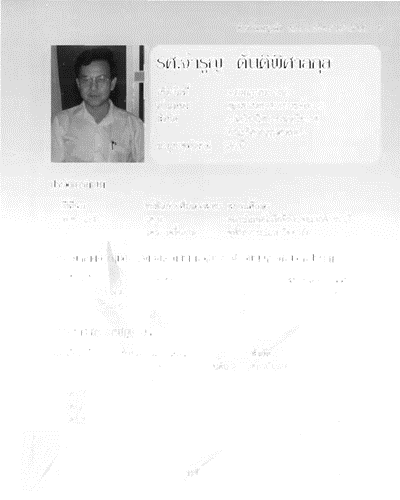
\includegraphics[scale=0.8]{rem3}
    \caption{รูปภาพที่ผ่านการทำการขยาย โดยใช้รูปแบบสี่เหลี่ยมขนาด 5x5}\label{fig:rem3}
\end{figure}

\begin{figure}[H]
    \centering
    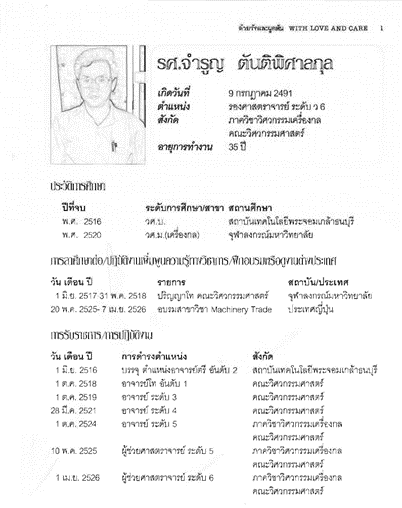
\includegraphics[scale=0.8]{rem4}
    \caption{รูปภาพที่ผ่านการลบพื้นหลัง}\label{fig:rem4}
\end{figure}

\begin{figure}[H]
    \centering
    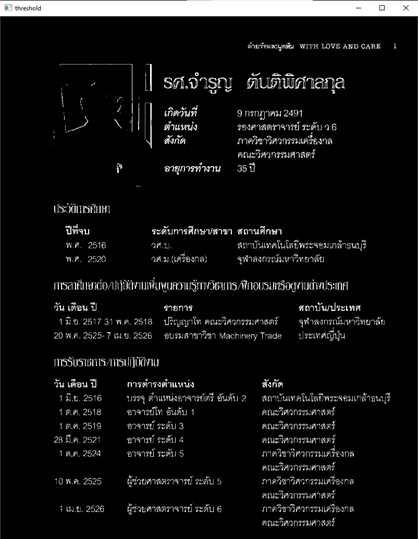
\includegraphics[scale=0.8]{rem5}
    \caption{รูปภาพที่ผ่านทำการ threshold แบบ THRESH\_BINARY\_INV}\label{fig:rem5}
\end{figure}

ในการลบพื้นหลังทางผู้จัดทำได้ทดลองใช้ขนาดไซส์ของ kernel ในขนาดต่างๆ โดยเปรียบเทียบ 3*3, 5*5, 7*7 และ 15*15 
ซึ่งจากการทดลองพบว่าขนาด kernel 3*3 นั้นจะทำให้ตัวอักษรที่ได้มีรูตรงกลาง ดังภาพที่ \ref{fig:3x3} และพอเพิ่มขนาดเป็น 5*5 7*7 
และ 15*15 จะเห็นได้ว่ายิ่งใช้ kernel ขนาดใหญ่ จะทำให้ตัวอักษรชัดมากยิ่งขึ้น แต่ถ้าเกิดใหญ่เกินไปก็จะทำให้เกิดจุดหรือเส้นรบกวนที่เกิดจากพื้นหลัง 
ตัวอักษรโดนสีขาวกลืนกินไปทำให้บางส่วนของตัวอักษรขาดหาย ดังภาพ \ref{fig:25x25} จึงตัด kernel ขนาด 3*3 และ 25*25 ทิ้งไป เหลือ 5*5, 7*7 
และ 15*15 ซึ่งจากผลลัพธ์ที่ได้เทียบระหว่าง 5*5 และ 7*7 จากภาพ\ref{fig:5x5} และ\ref{fig:7x7} นั้นไม่ต่างกันมากเราจึงเลือกใช้ขนาด 5*5 ก็เพียงพอส่วน kernel 15*15 นั้น มีขนาดที่ค่อนข้างใหญ่ 
ทำให้คาดว่าอาจจะทำให้เกิดการตัดประโยคมีความผิดพลาดมากยิ่งขึ้นดังภาพ \ref{fig:ker15x15} ดังนั้นจากการทดลองกับรูปภาพจึงทำให้ผู้จัดทำเลือกใช้ขนาด 5*5

\begin{figure}[H]
    \centering
    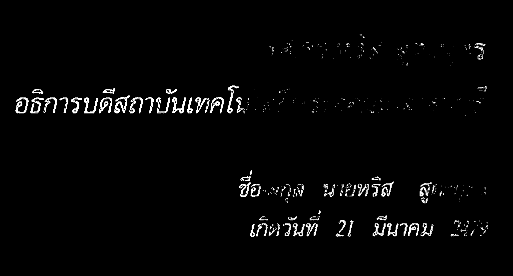
\includegraphics[scale=0.8]{3x3}
    \caption{รูปภาพแสดงการใช้การลบพื้นหลังด้วย kernel ขนาด 3*3}\label{fig:3x3}
\end{figure}

\begin{figure}[H]
    \centering
    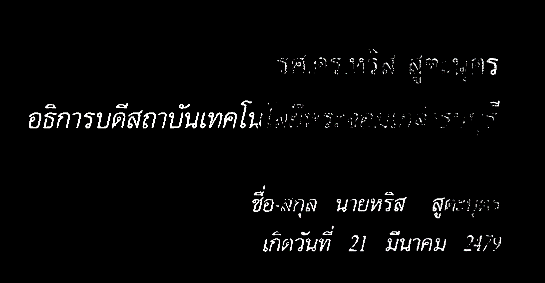
\includegraphics[scale=0.8]{5x5}
    \caption{รูปภาพแสดงการใช้การลบพื้นหลังด้วย kernel ขนาด 5*5}\label{fig:5x5}
\end{figure}

\begin{figure}[H]
    \centering
    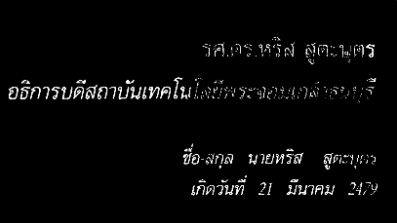
\includegraphics[scale=0.8]{7x7}
    \caption{รูปภาพแสดงการใช้การลบพื้นหลังด้วย kernel ขนาด 7*7}\label{fig:7x7}
\end{figure}

\begin{figure}[H]
    \centering
    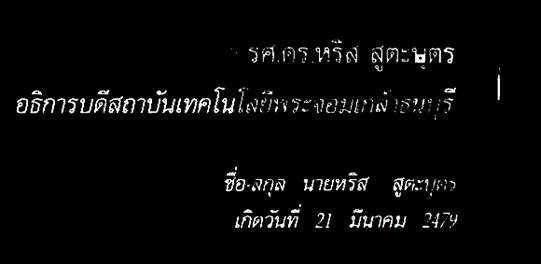
\includegraphics[scale=0.8]{15x15}
    \caption{รูปภาพแสดงการใช้การลบพื้นหลังด้วย kernel ขนาด 15*15}\label{fig:15x15}
\end{figure}

\begin{figure}[H]
    \centering
    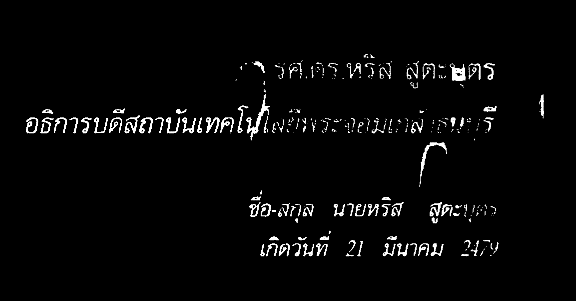
\includegraphics[scale=0.8]{25x25}
    \caption{รูปภาพแสดงการใช้การลบพื้นหลังด้วย kernel ขนาด 25*25}\label{fig:25x25}
\end{figure}

\begin{figure}[H]
    \centering
    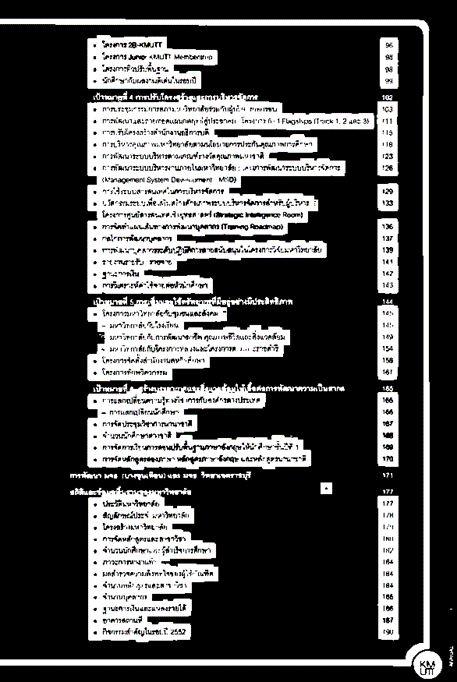
\includegraphics[scale=0.8]{ker15x15.png}
    \caption{รูปภาพแสดงการใช้การลบพื้นหลังด้วย kernel ขนาด 15*15 ที่กินพื้นที่รอบข้าง}\label{fig:ker15x15.png}
\end{figure}

\subsection{การแปลงข้อมูลรูปภาพให้อยู่ในรูปแบบดิจิทัล}

สำหรับการแปลงข้อมูลรูปภาพให้อยู่ในรูปแบบดิจิทัลจะใช้ Tesseract OCR โดยจะใช้รูปภาพที่ผ่านกระบวนการเตรียมข้อมูลรูปภาพและประโยคที่แปลงออกมาได้จัดเก็บไว้ใช้งานต่อไป

\subsection{การเตรียมข้อมูลตัวอักษร}

สำหรับการเตรียมข้อมูลตัวอักษรจัดทำเพื่อให้ข้อมูลเหมาะสมสำหรับการค้นหาเพื่อสร้างคำสำคัญของหนังสือ โดยเราจะนำหลักการของการทำ Tokenizer มาใช้ 
ซึ่งหลักการนี้จะมีรูปแบบแตกต่างกันออกไปในแต่ละภาษาที่จะใช้ โดยภาษาที่เราจะใช้มีภาษาไทย และภาษาอังกฤษ อันดับแรกของกระบวนการทำคือการตัดคำ
จากรูปประโยคซึ่งระหว่างแต่ละภาษาจะมีรูปแบบต่างกัน เราจึงต้องนำอัลกอรึทึมที่เรียกว่า Deepcut เข้ามาช่วยในการตัดแบ่งคำ หลังจากการตัดคำเราต้องจัด
การกับคำที่สื่อความหมายใกล้เคียงกันแต่รูปแบบการเขียนที่แตกต่างกันอย่าง รูปแบบตัวใหญ่ตัวเล็ก คำที่อยู่ในรูปนาม กริยา กรรมแต่สื่อความหมายถึงสิ่งเดียวกัน 
การจัดการคำที่ไม่มีความหมายแต่เป็นคำสำหรับรูปแบบการพูดเท่านั้น การแก้คำผิดสำหรับคำที่สแกนมาผิดพลาดให้กลายเป็นคำที่ถูกต้อง ซึ่งการเช็คคำในส่วนนี้จะ
ไม่สามารถเช็คคำเฉพาะได้อย่างเช่น ชื่อมหาวิทยาลัย ชื่อคน เราจึงต้องมีการเช็คคำเฉพาะอีกครั้ง และส่วนสุดท้ายผู้ใช้งานจะมีสิทธิในการเช็คคำอีกรอบในขั้นตอนสุดท้ายเพื่อลดการแก้คำผิดที่ไม่สามารถแก้ได้ทั้งหมด

\underline{ขั้นตอนการตัดแบ่งคำและการแก้ไขคำผิด}
\begin{enumerate}
    \item นำแต่ละประโยคในหน้านั้นมาทำการตัดคำโดยใช้อัลกอรึทึม Deepcut
    \item การจัดการตัวอักษรที่เราไม่ต้องการใช้และถือเป็นตัวอักษรที่ผิดพลาดที่เกิดจากการทำ OCR อย่างเช่น รูปแบบตัวอักษาลาติน ตัวอักษรที่เป็นรูปแบบสัญลักษณ์พิเศษ การจัดการรูปตัวอักษาตัวเล็กตัวใหญ่
    \item การค้นหาคำเฉพาะโดยการดูจากบริบทของคำ กรณีภาษาอังกฤษจะเป็นคำที่มีตัวอักษรแรกเป็นตัวใหญ่ และในกรณีของการใช้จุด “.” ของทั้งสองภาษาจะถือว่าเป็นคำเฉพาะเช่นเดียวกัน
    \item นำคำที่ถูกแยกออกมาจากรูปประโยคมาแก้ไขจากคำที่ผิดให้เป็นคำที่ถูกต้อง ซึ่งก่อนแก้ไขต้องระบุว่าคำที่จะแก้ไขเป็นภาษาชนิดใด โดยภาษาไทยจะมีวิธีการตรวจสอบโดยที่คำนั้นจะต้องมีทุกตัวอักษรเป็นภาษาไทยทั้งหมดจึงจะนับว่าเป็นภาษาไทย นอกเหนือจากนั้นจะนับเป็นภาษาอังกฤษทั้งหมด
    \item นำคำที่ถูกแก้คำแล้ว มาแก้คำเฉพาะอีกครั้งนึงเนื่องจากจะมีบางคำที่ไม่สามารถแก้ได้อย่าง ชื่อคนสำคัญ ชื่อมหาวิทยาลัย โดยใช้หลักการ Minimum edit distance
    \item นำผลลัพธ์ที่ได้ส่งไปยังขั้นตอนให้ผู้ใช้ตรวจสอบเพื่อเช็คคำผิดอีกครั้ง
    \item นำผลลัพธ์ที่ผู้ใช้งานตรวจสอบและแก้ไขมาทำการลบคำที่เป็น stop word
    \item นำผลลัพธ์ที่ได้จากการทำข้อที่ 7 เข้าสู่ระบบ

\end{enumerate}

\subsection{การคำนวณค่าความสำคัญของคำตามที่ปรากฎในเอกสาร}

หลังจากการเตรียมข้อมูลตัวอักษร จะนำผลลัพธ์ที่ได้จะนำเข้ากระบวนการคำนวณค่าความสำคัญของคำตามที่ปรากฎในเอกสาร โดยอัลกอรึทึม TF-IDF 
ซึ่งจะถูกเก็บในรูปแบบของ Inverted index ซึ่งในกรณีจากที่กล่าวจะเป็นรูปแบบการสร้างคำวำคัญ ของระบบที่สร้างเอง แต่จะมีในส่วนของการสร้างคำสำคัญ ที่ฝั่งผู้ใช้งานสามารถเพิ่มเข้าไปในระบบเองได้

\underline{ขั้นตอนการคำนวณค่าความสำคัญของคำตามที่ปรากฎในเอกสาร}
\begin{enumerate}
    \item นำคำที่ได้จากการเตรียมข้อมูลตัวอักษร มาทำการคำนวณผ่านอัลกอรึทึม TF-IDF เพื่อสร้างคะแนนขึ้นมา
    \item นำคำสำคัญผลลัพธ์ที่ได้มาให้ผู้ใช้ตรวจสอบใน 10 อันดับ และสามารถ เพิ่ม ลด แก้ไขได้ โดยที่ระบบจะทำการปรับแก้คะแนนของคำสำคัญที่ผู้ใช้งานจัดการในหนังสือ สามารถถูกค้นหาได้ง่ายกว่าคำสำคัญที่ระบบเป็นสร้างขั้นมาเอง
    
\end{enumerate}

\subsubsection{การอัพเดทค่าคะแนน TF-IDF}

เนื่องจากการที่มีหนังสือเพิ่มเข้ามาในระบบจะทำให้ผลลัพธ์คะแนน TF-IDF เปลี่ยนทั้งระบบจึงทำให้จำเป็นต้องมีการคำนวณใหม่เพื่อความแม่นยำในการค้นหาแต่เนื่องจาก
ถ้าระบบมีหนังสือจำนวนมากยิ่งขึ้นทางผู้จัดทำจึงปรับเปลี่ยนการอัพเดทคะแนนเป็น 1 ครั้งต่อวันโดยที่จะคำนวณคะแนนในช่วงเวลากลางคืนเพื่อไม่ให้ส่งผลกระทบกับผู้ใช้งาน 
และในส่วนการเพิ่มข้อมูลเข้ามาใหม่คำที่อยู่ภายในหนังสือนั้นจะถูกคำนวณและอัพเดทค่าใหม่ทันทีส่วนคำอื่นนั้นจะต้องรอเวลาที่กำหนดเพื่อที่จะอัพเดทค่า TF IDF และ TF-IDF 

\subsection{การค้นหา}

ในส่วนของระบบการค้นหานั้น จะมีระบบการกรองไว้ให้ผู้ใช้สามารถเลือกได้ว่าจะค้นหาหนังสือในหัวข้อไหน ซึ่งสามารถกรองหัวข้อได้มากกว่า 1 ครั้ง ต่อการค้นหา 1 รอบ 
โดยระบบการค้นหาจะถูกแบ่งออกเป็นสองส่วน ในส่วนแรกจะเป็นค้นหาในรูปแบบของ Cosine Similarity ซึ่งจะถูกทำ  Tokenizer เพื่อให้การค้นหาของผู้ใช้งานตรง
กับฐานข้อมูลมากที่สุด แต่จะไม่ทำการแก้ไขคำเพื่อไม่ให้จุดประสงค์ของการค้นหาถูกเปลี่ยนไปจากเดิม หลังจากนั้นการค้นหาในระบบยังสามารถค้นหาคำใกล้เคียงที่สื่อ
ความหมายแบบเดียวกันจากคำดั้งเดิมเพื่อที่จะได้ผลลัพธ์ที่ครอบคลุมหนังสือมากขึ้น และส่วนที่สองจะเป็นการกรองผลลัพธ์ทำให้ผู้ใช้สามารถลดผลลัพธ์ที่ไม่เกี่ยวข้อง
จำนวนมากให้ลดน้อยลงเพื่อง่ายต่อการค้นหา เมื่อผู้ใช้งานได้ทำการค้นหาเสร็จสิ้่นระบบจะทำการส่งหนังสือที่เกี่ยวข้องกับมาให้ผู้ใช้งาน

\underline{ขั้นตอนการทำระบบการค้นหา}

\begin{enumerate}
    \item แบ่งแยกประเภทการค้นหาของผู้ใช้ว่ามีค้นหา และการกรองทั้งหมดกี่รูปแบบ
    \item นำรูปประโยค หรือคำ จากรูปแบบการค้นหาที่ได้จากผู้ใช้ไปทำการ ตัดคำผ่าน Deepcut และหาคำที่มีความเหมือนจาก Word2Vec
    \item จากผลลัพธ์จะได้คำที่สามารถนำไปหาคะแนนเพื่อเข้ากระบวนการคิดแบบ Cosine Similarity ดังสมการ 3.1 และสามารถได้หนังสือที่เกี่ยวข้องพร้อมอันดับความเกี่ยวข้องของหนังสือนั้น ๆ
    \item จากผลลัพธ์จะได้หนังสือที่เกี่ยวข้อง ดังนั้นหากผู้ใช้ต้องการกรองผลลัพธ์เหล่านี้ระบบจะต้องนำหนังสือไปตรวจสอบว่าหนังสือใดบ้างที่ตรงตามเงื่อนไข
    \item นำผลลัพธ์ที่ได้ส่งคืนให้กลับผู้ใช้งาน
\end{enumerate}


\begin{equation}
    sim(\vec{q},\vec{d})=\frac{\sum_{i=1}^{|v|}q_{i}d_{i} }{\sqrt{\sum_{i=1}^{|v|}q^{2}_{i}x\sqrt{\sum_{i=1}^{|v|}d^{2}_{i}}}}
    \end{equation}    

\begin{figure}[H]
    \centering
    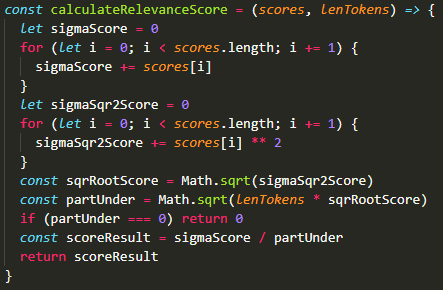
\includegraphics[scale=0.8]{cosinCode}
    \caption{รูปภาพแสดงการคำนวณ Cosine Similarity}\label{fig:cosinCode}
\end{figure}

\subsubsection{การทำโมเดล Word2vec}

โดยเราได้เตรียมข้อมูลที่จะนำมาสร้างโมเดลเป็นข้อมูลหนังสือกตเวทิตาและรายงานประจำปีของมหาวิทยาลัยเทคโนโลยีพระจอมเกล้าธนบุรี 
จำนวนทั้งหมด 44 เล่มโดยจะเป็นการนำข้อมูลที่ถูกกระบวนการ OCR และการเตรียมข้อมูลตัวอักษร มาตัดแบ่งคำเว้นช่องว่างและขึ้นบรรทัดใหม่ 
โดยจะใช้ Library genism ในสร้างโมเดลโดยมีการกำหนด window size เท่ากับ 2 และคำต้องมีกล่าวถึงมากกว่า 5 ครั้งโดยทำเป็นลักษณะ CBOW (Continuous Bag of Words)

\underline{ขั้นตอนการเตรียมข้อมูลที่นำมาสร้างโมเดล}

\begin{enumerate}
    \item เตรียมข้อมูลตัวอักษรโดยการนำแต่ละประโยคเข้ากระบวนการเตรียมข้อมูลตัวอักษร ในการตัดคำในรูปประโยค
    \item นำคำไปจัดการตัวอักษรที่เราไม่ต้องการใช้ และตรวจสอบแก้ไขคำผิดที่เกิดขึ้น
    \item ทำการเว้นช่องว่างระหว่างคำและขึ้นบรรทัดใหม่เมื่อขึ้นประโยคใหม่เพื่อที่เอาไว้ใช้งานสำหรับการสร้างโมเดล
    \item ทำการเขียนเพิ่มลงไปในไฟล์ corpus
    \item กำหนด parameter 
    \item เทรนโมเดล
\end{enumerate}

\subsection{การจัดการหนังสือดิจิทัล}

ในการจัดการข้อมูลหนังสือภายในระบบจะแบ่งทั้ง 3 ส่วนนั้นคือ 1. การเพิ่มหนังสือเข้าสู่ระบบ 2.การแก้ไขหนังสือภายในระบบ  3. การลบหนังสือออกจากระบบ 
ส่วนที่ 1. ในการเพิ่มหนังสือเข้าสู่ระบบ ผู้ใช้งานจะต้องอัปโหลดไฟล์หนังสือในรูปแบบ PDF และกรอกรายละเอียดของหนังสือเพื่อเข้าสู่กระบวนการแปลงข้อมูลในหนังสือ (Digitization) ต่อไปจะเป็นการเตรียมข้อมูลรูปภาพ ก่อนที่จะนำมาทำการแปลงภาพเป็นตัวอักษรเพื่อที่จะได้ข้อมูลดิจิทัลจากหนังสือที่ผู้ใช้เพิ่มเข้าสู่ระบบหลังจากนั้นจะเป็นการเตรียมข้อมูลตัวอักษร 
และให้ผู้ใช้งานได้ตรวจสอบคำอีกนึงครั้งก่อนที่นำคำเหล่านี้ไปผ่านกระบวนการสร้างคำสำคัญ เพื่อหาคำสำคัญในหนังสือโดยให้ผู้ใช้งานได้ตรวจสอบแก้ไขหรือเพิ่มเติมก่อนจะสิ้นสุดการเพิ่มหนังสือเข้าสู่ระบบ ในส่วนที่ 2 การแก้ไขหนังสือภายในระบบผู้ใช้งานสามารถค้นหาหนังสือภายในระบบเพื่อนำมาแก้ไขรายละเอียดที่ผู้ใช้งานกรอกเท่านั้นแต่มาสามารถแก้ไขคำที่ถูกแปลงออกมาเป็นดิจิทัลอีกครั้งได้ และส่วนสุดท้ายการลบหนังสือในระบบผู้ใช้งานสามารถลบหนังสือภายในระบบได้โดยการค้นหาหนังสือที่ต้องการและกดลบหนังสือนั้นออกจากระบบโดยเมื่อมีการลบหนังสือออกก็จะลบคำที่มีอยู่ในหนังสือออกไปจากระบบเช่นกัน

\subsection{Login}

ผู้ใช้งานสามารถเข้าสู่ระบบเพื่อใช้งานฟังก์ชั่นต่าง ๆภายในระบบโดยเมื่อผู้ใช้งานทำการเข้าสู่ระบบด้วยชื่อผู้ใช้งานและรหัสผ่านแล้วจะได้รับ “Token” เพื่อที่จะใช้สำหรับการยืนยันตัวในการใช้ฟังก์ชั่นต่าง ๆภายในระบบและผู้ใช้งานจะสามารถออกจากระบบได้

\section{System requirements}

\underline{ฝั่งผู้ใช้งาน}

ใช้งานได้บนระบบ web browser 

\begin{itemize}
    \item Google Chrome เวอร์ชั่น 84.0 ขึ้นไป 
    \item Microsoft Edge เวอร์ชั่น 83.0 ขึ้นไป
    \item Firefox เวอร์ชั่น 75.0 ขึ้นไป
\end{itemize}
 
\underline{ฝั่งเซิร์ฟเวอร์}
		
ทางด้านฮาร์ดแวร์

        \begin{itemize}
            \item CPU: Intel or AMD processor with 64-bit โดยที่ต้องมี 4 Core ขึ้นไป
            \item GPU: NVIDIA 1050ti or higher
            \item Disk Storage: 10 GB
            \item RAM: 8GB or higher
        \end{itemize}
        
		ทางด้าน Software แบ่งเป็น 2 ส่วนคือ Python และ JavaScript 
        \begin{enumerate}
            \item Python Backend
            \begin{itemize}
                \item Python เวอร์ชั่น 3.7.5
		        \item Tensorflow เวอร์ชั่น 2.3.1
		        \item DeepCut เวอร์ชั่น 0.7
		        \item Django เวอร์ชั่น 3.1.3
		        \item Djangorestframework เวอร์ชั่น 3.12.2
		        \item Django-cors-headers เวอร์ชั่น 3.5.0
		        \item PyThaiNLP เวอร์ชั่น 2.2.5
		        \item Pyspellchecker เวอร์ชั่น 0.5.5
		        \item nltk เวอร์ชั่น 3.5.0
		        \item mysqlclient เวอร์ชั่น 2.0.1
		        \item pillow เวอร์ชั่น 8.0.1
		        \item shapely เวอร์ชั่น 1.7.1
		        \item pytesseract เวอร์ชั่น 5.0.0 beta
		        \item opencv-python เวอร์ชั่น 4.4.0.46
		        \item pdf2image เวอร์ชั่น 1.14.0
		        \item scipy เวอร์ชั่น 1.5.4
            \end{itemize}
            \item JavaScript Backend and Frontend
		    \begin{itemize}
                \item nodejs เวอร์ชั่น 12.16.3
		        \item apollo-server-express เวอร์ชั่น 2.19.0
		        \item axios เวอร์ชั่น 0.20.0
		        \item cors เวอร์ชั่น 2.8.5
 		        \item dotenv เวอร์ชั่น 8.2.0
		        \item express เวอร์ชั่น 4.17.1
		        \item graphql เวอร์ชั่น 15.4.0
		        \item jsonwebtoken เวอร์ชั่น 8.5.1
		        \item knex เวอร์ชั่น 0.21.5
		        \item morgan เวอร์ชั่น 1.10.0
		        \item mysql2 เวอร์ชั่น 2.2.1
		        \item password-hash เวอร์ชั่น 1.2.2
		        \item react เวอร์ชั่น 16.13.1
		        \item react-hook-form เวอร์ชั่น 6.3.1
		        \item react-router-dom เวอร์ชั่น 5.2.0
		        \item styled-components เวอร์ชั่น 5.1.1
		        \item props-types เวอร์ชั่น 15.7.2
            \end{itemize}
        \end{enumerate}
		
\section{โครงสร้างฐานข้อมูล}

\begin{figure}[H]
    \centering
    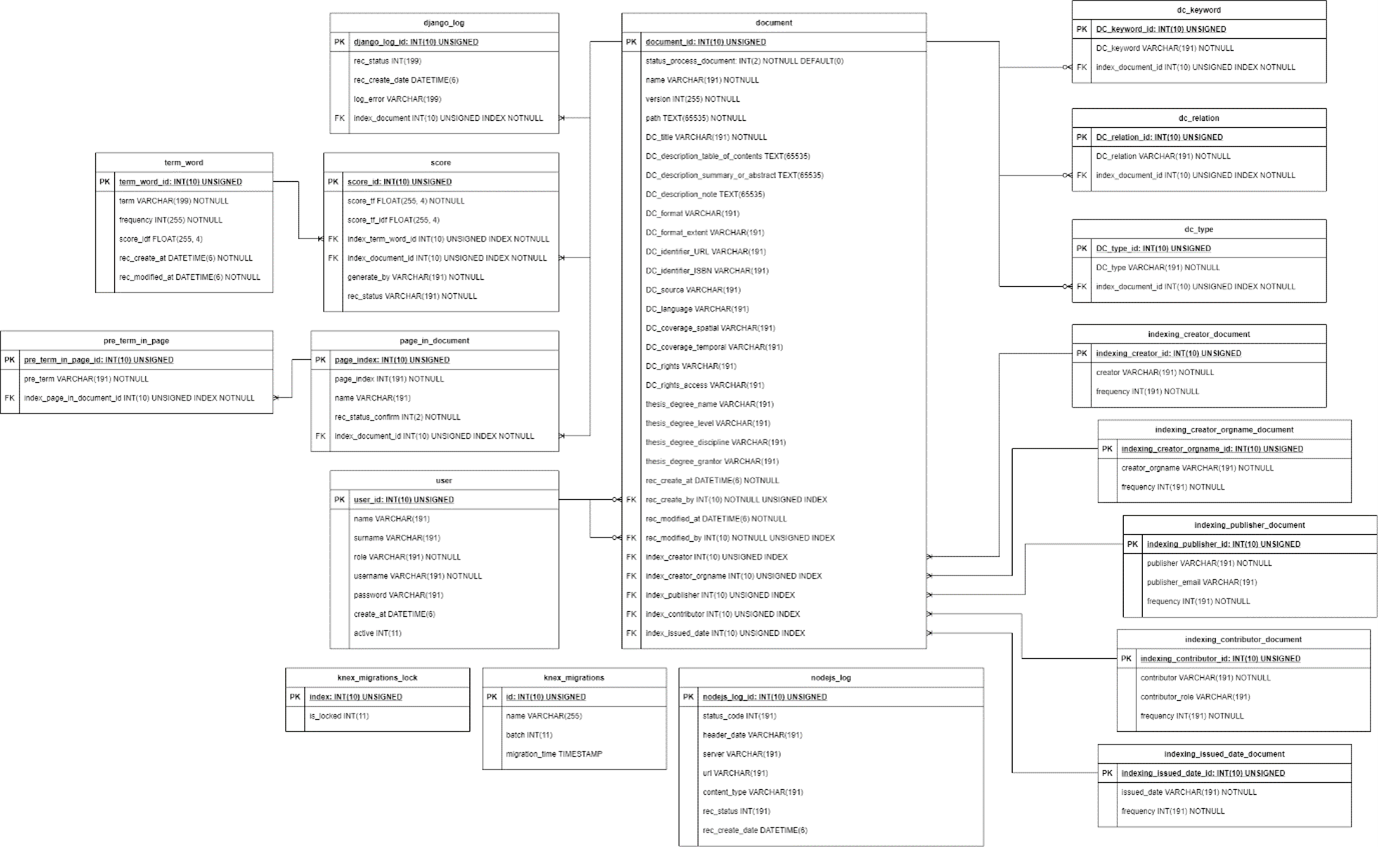
\includegraphics[scale=0.28]{er}
    \caption{แสดง ER Diagram ของฐานข้อมูล}\label{fig:er}
\end{figure}

\begin{figure}[H]
    \centering
    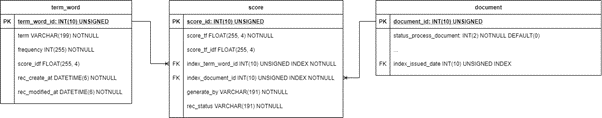
\includegraphics[scale=0.15]{er1}
    \caption{แสดง ER Diagram ส่วนของคีย์เวิร์ดและคะแนนความสำคัญในระบบ}\label{fig:er1}
\end{figure}


\begin{figure}[H]
    \centering
    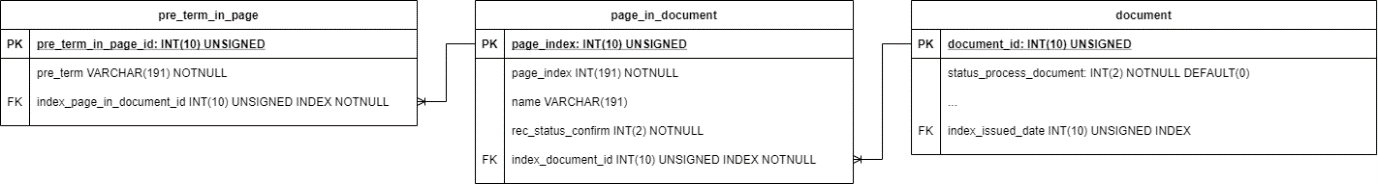
\includegraphics[scale=0.2]{er2}
    \caption{แสดง ER Diagram ส่วนของการเก็บคำจากแต่ละหน้าที่แปลงมาจากหนังสือ}\label{fig:er2}
\end{figure}


\begin{figure}[H]
    \centering
    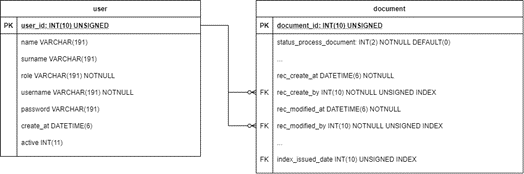
\includegraphics[scale=0.3]{er3}
    \caption{แสดง ER Diagram ส่วนของประวัติของผู้ใช้งานมีการสร้างหรือแก้ไขหนังสือ}\label{fig:er3}
\end{figure}



\begin{figure}[H]
    \centering
    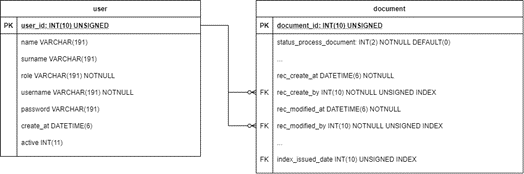
\includegraphics[scale=0.3]{er4}
    \caption{แสดง ER Diagram ส่วนของการเก็บข้อมูล keyword, relation, type ของหนังสือ}\label{fig:er4}
\end{figure}

\begin{figure}[H]
    \centering
    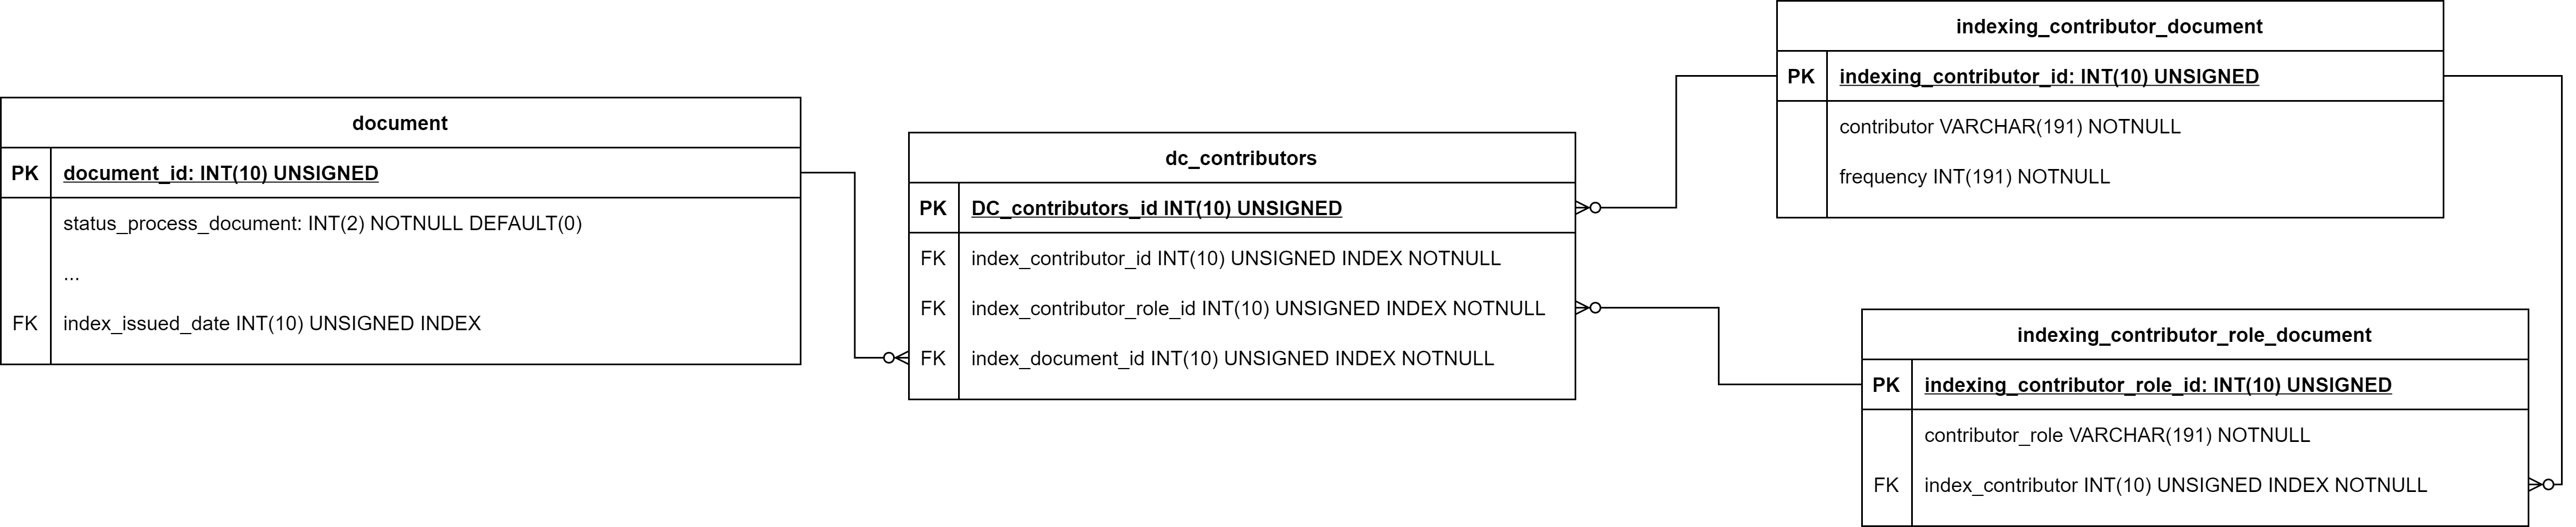
\includegraphics[scale=0.4]{er5}
    \caption{แสดง ER Diagram ส่วนของการเก็บข้อมูล Contributors ว่ามีความเกี่ยวข้องกับหนังสือไหรบ้าง}\label{fig:er5}
\end{figure}

\begin{figure}[H]
    \centering
    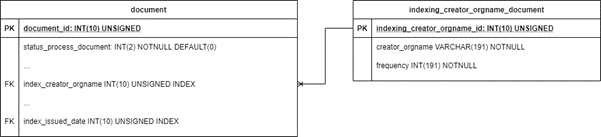
\includegraphics[scale=0.3]{er6}
    \caption{แสดง ER Diagram ส่วนของ Creator มีความเกี่ยวข้องกับหนังสือไหนบ้าง}\label{fig:er6}
\end{figure}



\begin{figure}[H]
    \centering
    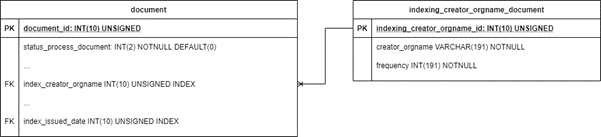
\includegraphics[scale=0.3]{er7}
    \caption{แสดง ER Diagram ส่วนของ Creator Organized Name มีความเกี่ยวข้องกับหนังสือไหนบ้าง}\label{fig:er7}
\end{figure}



\begin{figure}[H]
    \centering
    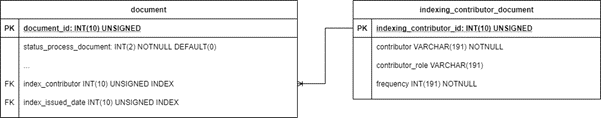
\includegraphics[scale=0.3]{er8}
    \caption{แสดง ER Diagram ส่วนของ Publisher มีความเกี่ยวข้องกับหนังสือไหนบ้าง}\label{fig:er8}
\end{figure}



\begin{figure}[H]
    \centering
    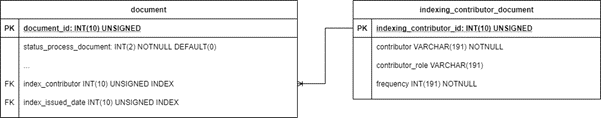
\includegraphics[scale=0.3]{er9}
    \caption{แสดง ER Diagram ส่วนของ Publisher Email มีความเกี่ยวข้องกับหนังสือไหนบ้าง}\label{fig:er9}
\end{figure}



\begin{figure}[H]
    \centering
    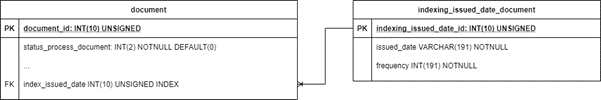
\includegraphics[scale=0.3]{er10}
    \caption{แสดง ER Diagram ส่วนของ Issued Date มีความเกี่ยวข้องกับหนังสือไหนบ้าง}\label{fig:er10}
\end{figure}



\begin{figure}[H]
    \centering
    \includegraphics[scale=0.5]{er11}
    \caption{แสดง ER Diagram ส่วนของ Knex module ที่ใช้สำหรับ Migration ฐานข้อมูล}\label{fig:er11}
\end{figure}



\begin{figure}[H]
    \centering
    \includegraphics[scale=0.5]{er12}
    \caption{แสดง ER Diagram ส่วนของการเก็บประวัติการ HTTP Request NodeJS ไปยัง Django}\label{fig:er12}
\end{figure}

\subsection{Database Structure}
รูปที่ \ref{fig:er} แสดงฐานข้อมูลของทั้งระบบโดยจะมีหลัก ๆ ทั้งหมดสามส่วน ทางด้านฝั่งขวาของตาราง document จะเป็นตารางที่เก็บข้อมูลเพิ่มเติมจากตาราง document และส่วนทางด้านฝั่งซ้ายของตาราง document สำหรับการเก็บข้อมูลในด้านของการทำระบบการเก็บคำจากหนังสือที่ถูกใส่ลงมาในระบบ ระบบการแปลงคำเป็นคีย์เวิร์ดและคะแนน TF-IDF ที่นำมาใช้สำหรับการค้นหาหนังสือ ระบบจัดการฐานข้อมูลผู้ใช้งาน และการตรวจสอบความผิดพลาดที่มีโอกาสจากการสร้างคีย์เวิร์ด และส่วนสุดท้ายที่เป็นตารางที่ไม่มีการเชื่อมโยงกับตารางใด ๆ จะมีไว้สำหรับการทำระบบฐานข้อมูล และระบบตรวจสอบ HTTP Request ของทาง NodeJS

รูปที่ \ref{fig:er1} จะเป็นส่วนของคีย์เวิร์ด และคะแนนเพื่อนำมาใช้สำหรับการค้นหาหนังสือของระบบนี้ โดยจะมีทั้งหมดสามตาราง document, term\_word, score ตาราง document จะเป็นตารางที่เก็บข้อมูลของหนังสือไว้ ส่วนตาราง term\_word จะเป็นการเก็บคีย์เวิร์ด และคะแนน IDF สำหรับการลดความสำคัญของคีย์เวิร์ดนั้น ๆ ไว้ซึ่งทั้งสองตารางนี้จะเป็นความสัมพันธ์แบบ one to many กับตาราง score ที่จะมีคะแนนสำหรับระบบการค้นหาเก็บเอาไว้ ที่มีความสัมพันธ์แบบนี้เนื่องจากในแต่ละคีย์เวิร์ดมีโอกาสพบได้ในหลายหนังสือ และหนังสือเองก็สามารถมีได้หลายคีย์เวิร์ด เนื่องจากแต่ละคีย์เวิร์ดที่อยู่ต่างหนังสือกันจะมีคะแนนไม่เท่ากัน

รูปที่ \ref{fig:er2} จะเป็นส่วนของการเก็บคำที่แปลงมาจากหนังสือไว้โดยเริ่มที่ตาราง document จะที่สามารถบอกได้ว่าหนังสือไหน ที่จะมีความพันธ์ one to many ไปยังตาราง page\_in\_document ที่จะเป็นตารางที่บอกถึงหน้าต่าง ๆ ในหนังสือนั้น และยังมีความสัมพันธ์ one to many ต่อไปยังตาราง per\_term\_in\_page ที่จะมีคำต่าง ๆ เก็บเอาไว้ ดังนั้นจะเป็นความสัมพันธ์ที่หนังสือนั้นจะสามารถมีได้หลายหน้า แล้วแต่ละหน้าเองก็จะมีคำต่าง ๆ ที่แปลงออกมาถูกเก็บเอาไว้

รูปที่ \ref{fig:er3} จะเป็นความสัมพันธ์ของบัญชีผู้ใช้กับหนังสือ โดยจะมีตาราง user ที่จะเก็บข้อมูลของผู้ใช้งานที่มีความสัมพันธ์แบบ one to many ไปยังตาราง document ที่จะเก็บต้องเก็บข้อมูลของผู้ใช้ไว้ว่าผู้ใช้คนไหนเป็นคนสร้าง หรือแก้ไขหนังสือนี้ ซึ่งบัญชีผู้ใช้สามารถสร้างหรือแก้ไขหนังสือได้หลายหนังสือ

รูปที่ \ref{fig:er4} จะเป็นส่วนของข้อมูลของตาราง Document เหมือนกันแต่เนื่องจากข้อมูลมีมากกว่าหนึ่งทำให้ต้องสร้างความสัมพันธ์แบบ one to many กับตาราง dc\_keyword, dc\_relation, dc\_type ซึ่งจะเป็นข้อมูลคีย์เวิร์ด ความสัมพันธ์ และประเภทของหนังสือตามลำดับ

รูปที่ \ref{fig:er5} จะเป็นการเก็บข้อมูลของ Contributor โดยจะมีตารางแยกเพื่อเก็บของสัมพันธ์ของทั้งสองด้านเนื่องจากในเอกสารสามารถมี contributor ได้หลายคน และ contributor สามารถมีหลายเอกสารเช่นกัน โดยที่ contributor จะมี role เป็นของตัวเองซึ่งสามารถมีหลาย role เช่นกันทำให้ต้องมีตาราง รองรับเพิ่ม แต่เนื่องจากในเอกสารเล่มนึงนั้น contributor จะสามารถมี role ได้แค่อย่างเดียวเท่านั้นดังนั้นจะเห็นว่ามีการเชื่อม role อีกครั้งเพื่อระบุให้แต่ละเอกสารอย่างเฉพาะเจาะจง

รูปที่ \ref{fig:er6} จะเป็นส่วนของการเก็บความสัมพันธ์ระหว่าง Creator กับหนังสือ เนื่องจาก Creator สามารถมีได้หลายหนังสือทำให้ตาราง indexing\_creator\_document จะเป็นความสัมพันธ์แบบ one to many กับตาราง document 

รูปที่ \ref{fig:er7} จะเป็นส่วนของการเก็บความสัมพันธ์ระหว่าง Creator orgname กับหนังสือเนื่อง จากCreator orgname สามารถมีได้หลายหนังสือทำให้ตาราง indexing\_creator\_orgname\_document จะเป็นความสัมพันธ์แบบ one to many กับตาราง document 

รูปที่ \ref{fig:er8} จะเป็นส่วนของการเก็บความสัมพันธ์ระหว่าง Publisher กับหนังสือ เนื่องจาก Publisher สามารถมีได้หลายหนังสือทำให้ตาราง indexing\_publisher\_document จะเป็นความสัมพันธ์แบบ one to many กับตาราง document 

รปที่ \ref{fig:er9} จะเป็นส่วนของการเก็บความสัมพันธ์ระหว่าง Publisher Email กับหนังสือ เนื่องจาก Publisher Email สามารถมีได้หลายหนังสือทำให้ตาราง indexing\_publisher\_email\_document จะเป็นความสัมพันธ์แบบ one to many กับตาราง document

รูปที่ \ref{fig:er10} จะเป็นส่วนของการเก็บความสัมพันธ์ระหว่าง Issued Date กับหนังสือ เนื่องจาก Issued Date สามารถมีได้หลายหนังสือทำให้ตาราง indexing\_issued\_date\_document จะเป็นความสัมพันธ์แบบ one to many กับตาราง document 

รูปที่ \ref{fig:er11} จะเป็นสองตารางที่บันทึกการจัดการฐานข้อมูลของเครื่องมือที่ชื่อว่า Knex ที่จะทำการจัดการสร้างฐานข้อมูล ด้วยคำสั่ง Migration แล้วหลังจากทำคำสั่งเสร็จสิ้นจะเก็บบันทึกไว้

รูปที่ \ref{fig:er12} จะเป็นตารางสำหรับการเก็บ HTTP Request จาก NodeJS ที่ส่งไปทางฝั่งของ Django ซึ่งจะถูกเก็บข้อมูลไว้ในตารางนี้

\subsection{Database Dictionary}

ในส่วนของการอธิบายถึงชื่อของคอลัมน์ ความหมายและลักษณะการเก็บข้อมูลภายในฐานข้อมูลโดยที่ตารางมีทั้งหมด 18 ตารางจะอยู่ในส่วนของภาคผนวก

\section{UML Design}
\subsection{Use case diagram}

\begin{figure}[H]
    \centering
    \includegraphics{usecasediagram}
    \caption{Use case diagram}\label{fig:usecasediagram}
\end{figure}

\subsection{Sequence diagram}

\subsubsection{Use case Add Document}

Scenario 1: เพิ่มหนังสือ/หนังสือเข้าสู่ระบบ

Goal: เพิ่มข้อมูลของหนังสือเข้าไปอยู่ในระบบ

Precondition: กดไปที่หัวข้อ INSERT BOOK ใน Web Application 

Main success scenario:

\begin{enumerate}
    \item อัพโหลดหนังสือ/หนังสือเลือกหน้าที่จะให้เริ่มต้นการแปลง
    \item กรอกข้อมูลรายละเอียดที่ต้องการลงในระบบ
    \item แสดงสถานะของการเพิ่มข้อมูล
    \item เพิ่มหนังสือ/หนังสือเข้าสู่ระบบ
\end{enumerate}

\begin{figure}[H]
    \centering
    \includegraphics{scene1}
    \caption{แสดง Scenario 1 เพิ่มหนังสือเข้าระบบ}\label{fig:scene1}
\end{figure}

\subsubsection{Use case Manage word in document}

Scenario 2: การตรวจสอบและแก้ไขคำก่อนนำเข้าสู่ระบบ

Goal: ผู้ใช้งานเห็นคำที่จะถูกการแปลงเป็นดิจิทัลแล้วสามารถจัดการคำเหล่านั้นได้

Precondition: อยู่ภายในขั้นตอนการเพิ่มหนังสือ/หนังสือลงในระบบ

Main success scenario:

\begin{enumerate}
    \item ผู้ใช้เข้าไปยังหน้าดูสถานะการเพิ่มหนังสือ
    \item ผู้ใช้เลือกหนังสือที่อยู่ในสถานะตรวจสอบคำ
    \item ระบบแสดงคำทั้งหมดที่ถูกแปลงมาได้จากหนังสือแต่ละหน้า
    \item ผู้ใช้ตรวจสอบ แก้ไขคำที่แสดงขึ้นมา
    \item ยืนยันขั้นตอนการตรวจสอบและแก้ไขคำ
\end{enumerate}
\begin{figure}[H]
    \centering
    \includegraphics{scene2}
    \caption{แสดง Scenario 2 การจัดการคำที่ถูกเก็บได้จากหนังสือในระบบ}\label{fig:scene2}
\end{figure}

\subsubsection{Use case Verify Document to Generate Keyword}

Scenario 3: ยื่นหนังสือว่าพร้อมสำหรับการถูกนำไปสร้างคียเวิร์ด

Goal: หนังสือถูกยืนยันพร้อมกับสร้างคีย์เวิร์ดเพื่อเพิ่มเข้าไปในระบบ

Precondition: ไปยังหน้าสถานะของหนังสือแล้วกดไปยังปุ่มยืนยันหนังสือถูกต้อง

Main success scenario:

\begin{enumerate}
    \item ผู้ใช้เข้าไปยังหน้าดูสถานะการเพิ่มหนังสือ
    \item ระบบแสดงสถานะหนังสือว่าหนังสือไหนอยู่สถานะใดแล้วบ้าง
    \item ผู้ใช้กดยืนยันว่าหนังสือถูกต้อง
    \item ระบบย้ายไปหน้าสถานะหนังสืออีกครั้งเพื่อรอผลการทำงาน
    \item ระบบแสดงการยืนยันหนังสือ และถูกเพื่อคีย์เวิร์ดเสร็จสิ้น
\end{enumerate}
\begin{figure}[H]
    \centering
    \includegraphics{scene3}
    \caption{แสดง Scenario 3 ยืนหนังสือว่าพร้อมสำหรับการถูกนำไปสร้างคีย์เวิร์ด}\label{fig:scene3}
\end{figure}

\subsubsection{Use case Edit Document}

Scenario 4: การแก้ไขรายละเอียดของหนังสือ/หนังสือที่อยู่ภายในระบบ

Goal: รายละเอียดหนังสือถูกแก้ไขตามผู้ใช้งานต้องการ

Precondition: กดไปที่หัวข้อ MANAGE BOOK ใน Web Application

Main success scenario:

\begin{enumerate}
    \item ผู้ใช้ค้นหาหนังสือที่ต้องการแก้ไขรายละเอียด
    \item แสดงผลลัพธ์ในการค้นหาหนังสือ/หนังสือ
    \item เลือกหนังสือ/หนังสือที่ต้องการแก้ไขรายละเอียด
    \item แก้ไขรายละเอียดที่ต้องการ
    \item กดบันทึกข้อมูลลงไปในระบบ
\end{enumerate}
\begin{figure}[H]
    \centering
    \includegraphics{scene4}
    \caption{แสดง Scenario 4 แก้ไขข้อมูลหนังสือ}\label{fig:scene4}
\end{figure}

\subsubsection{Use case Delete Document}

Scenario 5: ลบหนังสือ/หนังสือภายในระบบ

Goal: หนังสือ/หนังสือถูกนำออกจากระบบ

Precondition: กดเลือกหัวข้อ MANAGE BOOK ใน Web Application

Main success scenario:

\begin{enumerate}
    \item ผู้ใช้ทำการค้นหาหนังสือหนังสือที่ต้องการจะลบออกจากระบบ
    \item แสดงผลลัพธ์ในการค้นหาหนังสือ/หนังสือ
    \item กดลบหนังสือ/หนังสือที่ต้องการ
    \item กดยืนยันคำสั่งลบเพื่อบันทึกลงระบบ
\end{enumerate}
\begin{figure}[H]
    \centering
    \includegraphics{scene5}
    \caption{แสดง Scenario 5 ลบหนังสือ}\label{fig:scene5}
\end{figure}

\subsubsection{Use case View Document \& Search Document}

Scenario 6: ดูข้อมูลหนังสือ และการค้นหาหนังสือ

Goal: ผู้ใช้เจอหนังสือที่ต้องการ

Precondition: กดไปที่หัวข้อ SEARCH ใน Web Application

Main success scenario:

\begin{enumerate}
    \item กรอกรายละเอียดข้อมูลที่ต้องการจะค้นหา
    \item แสดงผลลัพธ์ในการค้นหา
    \item ผู้ใช้เลือกหนังสือที่ต้องการที่จะดูข้อมูล
    \item ระบบย้ายไปยังหน้าแสดงข้อมูลหนังสือที่ถูกเลือก
\end{enumerate}
\begin{figure}[H]
    \centering
    \includegraphics{scene6}
    \caption{แสดง Scenario 6 ดูข้อมูลหนังสือ และการค้นหาหนังสือ}\label{fig:scene6}
\end{figure}

\subsubsection{Use case Login}

Scenario 7: ระบบล็อกอิน

Goal: เพื่อเข้าสู่ระบบให้สามารถใช้ฟังก์ชั่นภายใน Web Application เพิ่มเติมได้

Precondition: กดหัวข้อ LOGIN ใน Web Application

Main success scenario:

\begin{enumerate}
    \item ผู้ใช้กรอกชื่อผู้ใช้งานและรหัสผ่าน
    \item กดเข้าสู่ระบบ
    \item เข้าสู่ระบบสำเร็จ ส่งผู้ใช้กลับไปสู่ Homepage
    \item สามารถเข้าใช้งานฟังก์ชั่นของ Web Application ได้
\end{enumerate}
\begin{figure}[H]
    \centering
    \includegraphics{scene7}
    \caption{แสดง Scenario 7 ระบบล็อกอิน}\label{fig:scene7}
\end{figure}

\section{GUI Design}

\subsection{Homepage}
\begin{figure}[H]
    \centering
    \includegraphics[scale=0.3]{hp}
    \caption{ภาพแสดงหน้าหลักของเว็บไซต์}\label{fig:hp}
\end{figure}
หน้าหลักของเว็บไซต์จะเป็นหน้าที่เน้นการค้นหาเป็นหลัก ที่ผู้ใช้สามารถเข้าถึงเมนูการเพิ่มหนังสือ การจัดการ และการเข้าสู่ระบบได้ที่แถบ Navigation ด้านบนของเว็บไซต์ดังรูปที่ \ref{fig:hp}

\subsection{Homepage2}
\begin{figure}[H]
    \centering
    \includegraphics[scale=0.3]{hp2}
    \caption{ภาพแสดงหน้าหลักของเว็บไซต์หลังจากการกดเปิดเมนู}\label{fig:hp2}
\end{figure}
เมื่อกดปุ่มลูกศรที่ด้านล่างของรูป \ref{fig:hp} จะมีเมนูเพิ่มเติมขึ้นมากลายเป็นรูปที่ \ref{fig:hp2} ซึ่งจะแสดงรายละเอียดในแต่ละฟังก์ชั่นเพิ่มเติม

\subsection{Login}
\begin{figure}[H]
    \centering
    \includegraphics[scale=0.3]{login}
    \caption{ภาพแสดงหน้าเข้าสู่ระบบ}\label{fig:scene7}
\end{figure}
ก่อนที่จะทำการเพิ่มหนังสือหรือจัดการกับหนังสือผู้ใช้นั้นจะต้องเข้าสู่ระบบก่อนเสมอ ถ้าเกิดกดเข้าฟังก์ชั่นการเพิ่มหนังสือหรือค้นหาโดยที่ยังไม่ได้เข้าสู่ระบบ ระบบจะบังคับให้ผู้ใช้เข้ามาในหน้าเข้าสู่ระบบดังรูป 3.25 เพื่อทำการเข้าสู่ระบบหรือจะเข้ามาโดยการกด log in ที่ปุ่มขวาบนได้

\subsection{Insert Book(1)}
\begin{figure}[H]
    \centering
    \includegraphics[scale=0.27]{i1}
    \caption{ภาพแสดงขั้นตอนการเพิ่มหนังสือเข้าสู่ระบบขั้นเลือกไฟล์}\label{fig:i1}
\end{figure}
หน้าเพิ่มหนังสือขั้นแรกจะเป็นการเลือกไฟล์หนังสือที่ต้องการโดยที่จะมีส่วนของการเพิ่มไฟล์ที่อยู่รูปของ pdf เพื่อทำ OCR จากนั้นจะสามารถเลือกได้ว่าจะทำการ OCR ตั้งแต่หน้าไหนดังรูปที่ 3.26

\subsection{Insert Book (2) }
\begin{figure}[H]
    \centering
    \includegraphics[scale=0.15]{i2}
    \caption{ภาพแสดงขั้นตอนการเพิ่มหนังสือเข้าสู่ระบบขั้นกรอกข้อมูลขั้นที่ 1}\label{fig:i2}
\end{figure}
หน้าเพิ่มหนังสือขั้นตอนที่ 2 เป็นหน้าที่ต้องใส่ข้อมูลที่จำเป็นของหนังสือ โดยที่จำเป็นต้องใส่จะมีสัญลักษณ์กำกับไว้หรือก็คือชื่อหนังสือดังรูป 3.27 โดยในหน้านี้จะมีกล่องใส่ข้อมูลที่ถูกกรอกบ่อย ๆสำหรับผู้ใช้(เจ้าหน้าที่)

\subsection{Insert Book (3)}
\begin{figure}[H]
    \centering
    \includegraphics[scale=0.3]{i3}
    \caption{ภาพแสดงขั้นตอนการเพิ่มหนังสือเข้าสู่ระบบขั้นกรอกข้อมูลขั้นที่ 2}\label{fig:i3}
\end{figure}
ในขั้นตอนที่ 3 จากรูปที่ 3.28 จะเป็นหน้าที่ใส่ข้อมูลที่ส่วนใหญ่ผู้ใช้จะไม่ค่อยกรอกมากนัก ซึ่งไม่มีกล่องข้อมูลไหนจำเป็นที่ต้องกรอกผู้ใช้สามารถข้ามไปขั้นตอนถัดไปได้เลย

\subsection{Insert Book (4)}
\begin{figure}[H]
    \centering
    \includegraphics[scale=0.3]{i4}
    \caption{ภาพแสดงขั้นตอนการเพิ่มหนังสือเข้าขั้นโหลดข้อมูลเข้าสู่ระบบ}\label{fig:i4}
\end{figure}
หลังจากที่ทำการใส่ข้อมูลออกมาทั้งหมดแล้วมาถึงหน้าที่เป็นหน้าโหลดข้อมูลดังรูป 3.29 ที่ระบบจะทำการ OCR และทำการเตรียมชุดข้อมูลที่ได้จากการ OCR โดยการนำคำมาตัดและเช็คคำผิด เมื่อโหลดข้อมูลเสร็จแล้วระบบจะทำการเปลี่ยนสถานะการโหลดและขึ้นลิ้งเพื่อเข้าสู่ขั้นตอนถัดไปได้

\subsection{Insert Book (5)}
\begin{figure}[H]
    \centering
    \includegraphics[scale=0.3]{i5}
    \caption{ภาพแสดงขั้นตอนการเพิ่มหนังสือเข้าสู่ระบบขั้นแก้ไขคำผิด}\label{fig:i5}
\end{figure}
หลังจากโหลดและเตรียมข้อมูลเรียบร้อยแล้ว ระบบจะทำการแสดงข้อมูลที่ถูกแปลงมาโดยที่ผู้ใช้จะสามารถแก้ไขคำได้ดังรูป 3.30 หรือสามารถข้ามได้เลยเช่นกัน โดยเมื่อคลิกไปที่กล่องข้อความจะขึ้นให้แก้แต่ละคำและเมื่อเปลี่ยนหน้าจะทำการเก็บข้อมูลที่เปลี่ยนไว้ และจะบันทึกการแก้ไขข้อมูลทั้งหมดที่แก้เมื่อข้ามไปขั้นตอนถัดไป

\subsection{Insert Book (6) }
\begin{figure}[H]
    \centering
    \includegraphics[scale=0.3]{i6}
    \caption{ภาพแสดงขั้นตอนการเพิ่มหนังสือเข้าสู่ระบบขั้นแก้ไขและเพิ่มคำสำคัญ}\label{fig:i6}
\end{figure}
หน้าสุดท้ายของการเพิ่มหนังสือจะเป็นหน้าที่ให้ผู้ใช้สามารถจัดการกับ Keyword ได้ดังรูปที่ 3.31 โดยเมื่อผู้ใช้ต้องการใส่คำสำคัญเพิ่มสามารถกด ADD เพื่อเพิ่มคำที่ต้องการใส่ได้ และสามารถลบเมื่อคลิกที่ปุ่มกากบาทที่คำสำคัญที่ระบบทำการสร้างมาให้ เมื่อแก้ไขเสร็จแล้วสามารถกดปุ่ม Finish เพื่อทำการบันทึกข้อมูล

\subsection{Search}
\begin{figure}[H]
    \centering
    \includegraphics[scale=0.3]{search}
    \caption{ภาพแสดงหน้าค้นหาข้อมูล}\label{fig:search}
\end{figure}
หน้าแสดงข้อมูลการค้นหาเมื่อทำการค้นหาข้อมูลจากหน้าแรก (รูปที่ 3.23 หรือ 3.24) จะทำการแสดงข้อมูลหนังสือที่ตรงกับ Keyword โดยเรียงคะแนนของหนังสือที่เกี่ยวข้องกับคำค้นหามากที่สุดดังรูปที่ 3.32 เมื่อกดเข้าไปที่รายชื่อหนังสือจะทำการนำทางผู้ใช้ไปยังหน้าดูหนังสือดังรูปที่ 3.33

\subsection{Document View}
\begin{figure}[H]
    \centering
    \includegraphics[scale=0.3]{lookupp}
    \caption{ภาพแสดงหน้าดูหนังสือ}\label{fig:lookupp}
\end{figure}
เมื่อเราค้นหาและเลือกหนังสือ ก็จะมีหน้าหนังสือ (รูปที่ 3.33) ขึ้นมาให้ดูเนื้อหาภายในโดยที่ผู้ใช้สามารถปรับขนาดภาพและสามารถเลือกหน้าที่ต้องการจะเปิดได้และสามารถย้อนหลับไปยังหน้าเสริชได้ที่ปุ่มลูกศรทางด้านซ้ายบน

\subsection{Manage book}
\begin{figure}[H]
    \centering
    \includegraphics[scale=0.3]{man1}
    \caption{ภาพแสดงหน้าการจัดการหนังสือที่เพิ่มเข้าสู่ระบบ}\label{fig:man1}
\end{figure}
ในหน้าของการจัดการหนังสือดังรูปที่ 3.34 จะมีลักษณะคล้ายกับหน้าการค้นหาเพียงแต่ว่าจะมีฟังก์ชั่นสำหรับการแก้ไขเนื้อหนังสือภายในที่ผู้ใช้เคยกรอกไว้ตอน OCR หนังสือมา เมื่อกดปุ่มลบจะมีหน้าต่างแจ้งเตือนเพื่อถามความแน่ใจในการลบหนังสือ หรือกดปุ่ม Edit เพื่อทำการเข้าสู่การแก้ไขข้อมูลของหนังสือนั้นๆดังรูปที่ 3.35 - 3.37

\subsection{Edit Book}
\begin{figure}[H]
    \centering
    \includegraphics[scale=0.15]{e1}
    \caption{ภาพแสดงขั้นตอนการแก้ไขหนังสือขั้นที่ 1}\label{fig:e1}
\end{figure}

\begin{figure}[H]
    \centering
    \includegraphics[scale=0.3]{e2}
    \caption{ภาพแสดงขั้นตอนการแก้ไขหนังสือขั้นที่ 2}\label{fig:e2}
\end{figure}

\begin{figure}[H]
    \centering
    \includegraphics[scale=0.3]{e3}
    \caption{ภาพแสดงขั้นตอนการแก้ไขหนังสือขั้นที่ 3}\label{fig:e3}
\end{figure}

หน้าแก้ไขหนังสือแบ่งออกเป็น 3 ขั้นตอนดังรูป 3.35 - 3.37 ซึ่งจะมีให้แก้ไข ข้อมูลที่เคยกรอกไว้ตอนเพิ่มหนังสือเข้ามา โดยจะมีรูปปกหนังสือและชื่อหนังสือคอยบอกว่ากำลังแก้ไขหนังสือเล่มไหนอยู่ และในทุกหน้าจะมีปุ่มสำหรับบันทึกในทุกหน้าเพื่อที่จะสามารถบันทึกโดยที่ไม่ต้องรอไปหน้าสุดท้ายเพื่อบันทึกข้อมูล

\subsection{Upload Status Page}
\begin{figure}[H]
    \centering
    \includegraphics[scale=0.3]{status}
    \caption{ภาพแสดงหน้าการโหลดข้อมูล}\label{fig:status}
\end{figure}
จากรูป 3.38 สำหรับผู้ใช้ที่ทำการเพิ่มหนังสือเข้าสู่ระบบจะมีหน้าสำหรับโหลดกรณีที่กดออกมาหลังจากผ่านขั้นตอนการเพิ่มหนังสือขั้นตอนที่ 4 จะสามารถเข้ามาดูสถานะและทำการดำเนินการต่อได้โดยไม่ต้องผ่านการเพิ่มหนังสือเข้าสู่ระบบใหม่


\subsection{Evaluate Process Design}

ในส่วนของการประเมินผลการทำงานนั้นจะแบ่งออกเป็น 3 ส่วนคือการออกแบบ User Interface ส่วนของการเตรียมข้อมูลรูปภาพ จะช่วยให้การทำ OCR มีประสิทธิภาพมากเท่าไร และส่วนของระบบการค้นหา โดยในส่วนของ OCR จะทำการประเมินจากการเลือกเช็คคำจาก 2 หน้าของแต่ละหนังสือมาเช็คว่าแต่ละหน้ามีคำผิดเท่าไร โดยจะเลือกวัดหนังสือทั้งหมด 5 เล่มแบบสุ่มและเทียบการเตรียมข้อมูลรูปภาพ ว่าทำแบบไหนได้ผลลัพธ์แบบไหนออกมา

\begin{table}[H]
\caption{ตารางประเมินการทำ OCR}\label{tbl:ocr}
\begin{tabular}{|c|c|c|c|c|}
\hline
\multicolumn{5}{|c|}{ตารางประเมินการทำ OCR}                 \\ \hline
หนังสือ & หน้า & จำนวนคำทั้งหมด & คำที่ผิด(\%) & คำเกิน(คำ) \\ \hline
        &      &                &              &            \\ \hline
\end{tabular}
\end{table}

ระบบการค้นหา จะเช็คโดยให้ผู้ใช้เป็นผู้ประเมินว่าได้รับหนังสือตรงตามที่ต้องการหรือไม่โดยจะให้เจ้าหน้าที่บรรณารักษ์คัดเลือกหนังสือจำนวน 3 เล่มที่คาดหวังว่าจะขึ้นมาเมื่อค้นหาทั้งหมด 10 ครั้ง

\begin{table}[H] 
\caption{ตารางประเมินระบบการค้นหา}\label{tbl:searchtest}

\begin{tabular}{|c|l|l|}
    \hline
    \multicolumn{3}{|c|}{ตารางประเมินระบบการค้นหา} \\ \hline
    คำค้นหา &
      \multicolumn{1}{c|}{หนังสือที่คาดหวัง} &
      \multicolumn{1}{c|}{การค้นหา} \\ \hline
    \multicolumn{1}{|l|}{} &
       &
      \begin{tabular}[c]{@{}l@{}}คะแนน 5 ระดับ\\ 5   =  ค้นหาหนังสือได้ตรงตามที่ต้องการทั้งหมด  \\และไม่มีหนังสือที่ไม่เกี่ยวข้องกับคำค้นหาขึ้นมา\\ 4   = ค้นหาหนังสือได้ตรงตามที่ต้องการทั้งหมด \\และมีหนังสือที่ไม่เกี่ยวข้องกับคำค้นหาขึ้นมาบ้าง\\ 3   = ค้นหาหนังสือได้ตรงตามที่ต้องการบ้าง \\แต่ไม่มีหนังสือที่ไม่เกี่ยวข้องกับคำค้นหาขึ้นมา\\ 2 = ค้นหาหนังสือได้ตรงตามที่ต้องการบ้าง \\แต่มีหนังสือที่ไม่เกี่ยวข้องกับคำค้นหาขึ้นมาบ้าง\\ 1 = ไม่มีหนังสือที่ต้องการขึ้นมาในผลลัพธ์ \\หรือขึ้นหนังสือทุกเล่ม\end{tabular} \\ \hline
    \end{tabular}
    \end{table}


\begin{table}[H]
\caption{ตารางประเมินความพึงพอใจการออกแบบ UX/UI}\label{tbl:uxuieva}
\begin{tabular}{|p{0.13\linewidth}|p{0.17\linewidth}|p{0.17\linewidth}|p{0.17\linewidth}|p{0.17\linewidth}|c|}
\hline
\multicolumn{6}{|c|}{ตารางประเมินการออกแบบ UX/UI}                                                                                                                                                            \\ \hline

                     & \multicolumn{1}{c|}{4}                                                                                                 & \multicolumn{1}{c|}{3}                                                                                   & \multicolumn{1}{c|}{2}                                                                                        & \multicolumn{1}{c|}{1}                                                                        & คะแนนที่ได้ \\ \hline
ความสมบูรณ์ของข้อมูล    & ข้อมูลมีความสมบูรณ์   ชัดเจนทำให้เข้าใจความหมายที่ต้องการจะสื่อได้เป็นอย่างดี                                          & มีข้อมูลที่ชัดเจน   และแม่นยำในบางครั้ง และสามารถแสดงความหมายที่ต้องการจะสื่อได้บ้าง                     & ข้อมูลมีความแม่นยำ   และชัดเจนบ้าง                                                                            & มีข้อมูลที่ไม่ชัดเจน   ไม่ครบ สื่อความหมายได้ไม่ดี                                            &           \\ \hline
การออกแบบ            & มีการออกแบบที่เน้นความสำคัญและจัดวางองค์ประกอบ สี เสียง และการเคลื่อนไหว(animation) ได้อย่างเหมาะสม                                & มีการจัดหน้า   และองค์ประกอบทำให้เห็นใจความสำคัญของเนื้อหา มีการใช้การเคลื่อนไหว(animation)   บ้าง                     & การวางหน้าและการจัดองค์ประกอบมีความไม่เหมาะสม   มีการใช้การเคลื่อนไหว(animation) เข้ามาช่วยบ้าง                             & การวางหน้าและการจัดองค์ประกอบมีความไม่เหมาะสมและไม่มีการใช้  การเคลื่อนไหว(animation) เข้ามาช่วยในการใช้งาน &            \\ \hline
การใช้งาน              & ผู้ใช้สามารถใช้งานปุ่มหรือย้ายไปยังหน้าต่างๆได้อย่างง่ายดาย   แต่มีลิ้งค์ที่พาไปผิดหน้าอย่างมากหนึ่งลิ้งค์หรือไม่มีเลย & ผู้ใช้สามารถใช้งานปุ่มหรือย้ายไปยังหน้าต่างๆได้อย่างง่ายดาย   แต่มีลิ้งค์ที่พาไปผิดหน้าอย่างมากสองลิ้งค์ & ผู้ใช้มีความสับสนในการใช้ปุ่ม   หรือการย้ายไปยังหน้าต่างๆ บางครั้ง และมีลิ้งค์ที่พาไปผิดหน้าอย่างมากสามลิ้งค์ & ผู้ใช้เกิดความสับสนในปุ่มหรือลิ้งค์ที่ย้ายไปหน้าต่างๆ                                         &            \\ \hline
การใช้ภาษา            & มีการใช้คำผิดหรือภาษาที่ไม่เหมาะสมอย่างมาก   1 จุด                                                                     & มีการใช้คำผิดหรือภาษาที่ไม่เหมาะสมอย่างมาก   2 จุด                                                       & มีการใช้คำผิดหรือภาษาที่ไม่เหมาะสมอย่างมาก 3 จุด                                                              & มีการใช้คำผิดหรือภาษาที่ไม่เหมาะสมมากกว่า 4 จุด                                               &            \\ \hline
\end{tabular}
\end{table}

\begin{table}[H]
\caption{ตารางประเมินการทดสอบเว็บไซต์}\label{tbl:test}
\begin{tabular}{|l|l|l|l|}
\hline
\multicolumn{4}{|c|}{ตารางประเมินเว็บไซต์}                                                                                                                                             \\ \hline
\multicolumn{1}{|c|}{\multirow{2}{*}{เกณฑ์การประเมิน}}                  & \multicolumn{2}{c|}{ผลลัพธ์}                             & \multicolumn{1}{c|}{\multirow{2}{*}{หมายเหตุ}} \\ \cline{2-3}
\multicolumn{1}{|c|}{}                                                  & \multicolumn{1}{c|}{ผ่าน} & \multicolumn{1}{c|}{ไม่ผ่าน} & \multicolumn{1}{c|}{}                          \\ \hline
1. สามารถเข้าสู่ระบบและออกจาก ระบบได้                                   &                           &                              &                                                \\ \hline
2. สามารถเพิ่มหนังสือเข้าสู่ระบบได้                                      &                           &                              &                                                \\ \hline
3. สามารถแก้ไขรายละเอียดหนังสือที่อยู่ในระบบได้                          &                           &                              &                                                \\ \hline
4.   สามารถตรวจสอบและแก้ไขคำที่เพิ่มเข้ามาในระบบในขั้นตอนเพิ่มหนังสือได้ &                           &                              &                                                \\ \hline
5. สามารถลบหนังสือที่อยู่ในระบบได้                                       &                           &                              &                                                \\ \hline
6.   สามารถค้นหาข้อมูลหนังสือภายในระบบได้                                &                           &                              &                                                \\ \hline
7.   สามารถเรียกดูหนังสือที่ต้องการได้                                   &                           &                              &                                                \\ \hline
\end{tabular}
\end{table}
\chapter{ผลการดำเนินงาน}

การดำเนินงานของโปรเจคนี้จะแบ่งออกมาเป็นทั้งหมด 3 ส่วน โดยส่วนแรกคือส่วนของการจัดเก็บข้อมูลเข้าสู่ระบบโดยนำรูปภาพได้ที่ได้รับมาผ่านกระบวนการการเตรียมข้อมูลรูปภาพ 
ก่อนจะนำไปผ่านกระบวนการ OCR และการเตรียมข้อมูลตัวหนังสือ ก่อนจะถูกเก็บข้อมูลในระบบ ส่วนที่สองการค้นหาข้อมูล เป็นการค้นหาแบบ IR (Information retrieval) 
ที่จะนำไปโมเดล Word2Vec เข้ามาช่วยในการค้นหาคำที่มีความสัมพันธ์ใกล้เคียงกับคำค้นหา และนำคะแนน TF-IDF มาใช้เป็นคะแนนในการค้นหา และส่วนสุดท้ายคือส่วนของการทำแพลตฟอร์มเว็ปไซต์
ซึ่งในการประเมินผลการดำเนินงานนั้นเราจะทำการประเมินในส่วนแรก โดยการประเมินความถูกต้องของการทำ OCR จะมีเจ้าหน้าที่บรรณารักษ์กำหนดเกณฑ์ไว้ 
ซึ่งเกณฑ์ที่กำหนดในส่วนของความถูกต้องในการทำ OCR อยู่ที่ 75 \% และความแม่นยำในการค้นหาอยู่ที่ 75 \%

\section{ผลลัพธ์ที่ได้จากการแปลงข้อมูลรูปภาพให้เป็นข้อมูลดิจิทัล}

\subsection{ผลลัพธ์ที่ได้จากประสิทธิภาพของการหมุน}
ผลลัพธ์จากการหมุนภาพตัวหนังสือทั้ง 978 ภาพ มีความคลาดเคลื่อนทั้งหมด 7.98\% ที่ยังไม่สามารถหมุนภาพให้ตรงดังภาพที่ \ref{fig:rotateErrror} 
และทำให้บางภาพแย่ลง เนื่องจากว่าบรรทัดตัวอักษรอาจจะมีสระที่ไม่สามารถทำกร่อนให้กลายเป็นเส้นบรรทัดได้

\begin{figure}[H]
    \centering
    \includegraphics[scale=0.4]{rotateres}
    \caption{ภาพแสดงผลลัพธ์การหมุนรูปที่ถูกต้อง}\label{fig:rotateres}
\end{figure}

\begin{figure}[H]
    \centering
    \includegraphics[scale=1]{rotateErrror}
    \caption{ภาพแสดงผลลัพธ์การหมุนรูปที่ผิดพลาด}\label{fig:rotateErrror}
\end{figure}

\subsection{ผลการเปรียบเทียบประสิทธิภาพในการทำ OCR ของ การทำการเตรียมข้อมูลรูปภาพ แต่ละแบบ}

จากการทดสอบประสิทธิภาพของการทำการเตรียมข้อมูลรูปภาพทั้งสองแบบพบว่า การทำการเตรียมข้อมูลรูปภาพ แบบแรกนั้นมีจำนวนคำผิดน้อยกว่า แต่มีจำนวนคำที่ไม่สามารถแปลงเป็นดิจิทัลมากถึง 32.71\% ดังตารางที่ \ref{tbl:imagep1} ซึ่งต่างจากการทำการเตรียมข้อมูลรูปภาพ แบบที่ 2 ที่มีค่าความถูกต้องของคำ 74.74 \% ดังตาราง \ref{tbl:imagep2}

\subsubsection{แบบที่ 1 การใช้การคัดเลือกข้อมูล,การหมุน,การลบรูปภาพ,การลบเส้น และการจัดกลุ่ม}
\begin{table}[H]
    \caption{ตารางประเมินการทำการเตรียมข้อมูลรูปภาพแบบที่ 1 }\label{tbl:imagep1}
    \begin{tabular}{|c|c|c|p{0.1\linewidth}|p{0.1\linewidth}|c|p{0.1\linewidth}|p{0.1\linewidth}|}
        \hline
        หนังสือ                             & หน้า  & จำนวนคำทั้งหมด & จำนวนคำผิดที่ตรวจพบ & เปอร์เซ็นต์คำผิดที่ตรวจพบ(\%)    & จำนวนคำเกิน & จำนวนคำที่ไม่สามารถแปลงเป็นดิจิทัล & เปอร์เซ็นต์คำที่ไม่สามารถแปลงเป็นดิจิทัล(\%)    \\ \hline
        \multirow{2}{*}{กตเวทิตาปี 2542}      & 15    & 4         & \multicolumn{1}{c|}{4  }         & \multicolumn{1}{c|}{100 \%  } & \multicolumn{1}{c|}{0  }    & \multicolumn{1}{c|}{0  }             & \multicolumn{1}{c|}{0 \%    }\\ \cline{2-8} 
                                            & 29    & 252       & \multicolumn{1}{c|}{14 }         & \multicolumn{1}{c|}{5.56 \% }  &\multicolumn{1}{c|}{46}     &\multicolumn{1}{c|}{2 }              &\multicolumn{1}{c|}{0.79 \%} \\ \hline
        \multirow{2}{*}{กตเวทิตาปี 2556}      & 15    & 242       & \multicolumn{1}{c|}{33 }         & \multicolumn{1}{c|}{13.64 \%}  &\multicolumn{1}{c|}{2 }     &\multicolumn{1}{c|}{1 }              &\multicolumn{1}{c|}{0.41 \%} \\ \cline{2-8} 
                                            & 29    & 257       & \multicolumn{1}{c|}{20 }         & \multicolumn{1}{c|}{7.78 \% } & \multicolumn{1}{c|}{3  }    & \multicolumn{1}{c|}{10 }             & \multicolumn{1}{c|}{3.89 \% }\\ \hline
        \multirow{2}{*}{รายงานประจำปี 2544}   & 15    & 47        & \multicolumn{1}{c|}{3  }         & \multicolumn{1}{c|}{6.38 \% } & \multicolumn{1}{c|}{2  }    & \multicolumn{1}{c|}{34 }             & \multicolumn{1}{c|}{72.34 \%} \\ \cline{2-8} 
                                            & 29    & 585       & \multicolumn{1}{c|}{39 }         & \multicolumn{1}{c|}{6.67 \% } & \multicolumn{1}{c|}{3  }    & \multicolumn{1}{c|}{308}             & \multicolumn{1}{c|}{52.65 \%} \\ \hline
        \multirow{2}{*}{รายงานประจำปี 2553}   & 15    & 68        & \multicolumn{1}{c|}{0  }         & \multicolumn{1}{c|}{0 \%    } & \multicolumn{1}{c|}{0  }    & \multicolumn{1}{c|}{68 }             & \multicolumn{1}{c|}{100 \%  }\\ \cline{2-8} 
                                            & 29    & 596       & \multicolumn{1}{c|}{17 }         & \multicolumn{1}{c|}{2.85 \% } & \multicolumn{1}{c|}{8  }    & \multicolumn{1}{c|}{340}             & \multicolumn{1}{c|}{57.05 \%} \\ \hline
        \multirow{2}{*}{รายงานประจำปี 2549}   & 15    & 155       & \multicolumn{1}{c|}{53 }         & \multicolumn{1}{c|}{34.19 \%}  &\multicolumn{1}{c|}{42}     &\multicolumn{1}{c|}{45}              &\multicolumn{1}{c|}{29.03 \%} \\ \cline{2-8} 
                                            & 29    & 304       & \multicolumn{1}{c|}{22 }         & \multicolumn{1}{c|}{7.24 \% } & \multicolumn{1}{c|}{20 }    & \multicolumn{1}{c|}{13 }             & \multicolumn{1}{c|}{4.28 \%}\\ \hline
        \multicolumn{1}{|l|}{}              & total & 2510      & \multicolumn{1}{c|}{205}         & \multicolumn{1}{c|}{8.17 \% } & \multicolumn{1}{c|}{126}    & \multicolumn{1}{c|}{821}             & \multicolumn{1}{c|}{32.71 \%} \\ \hline
        \end{tabular}
        \end{table}

\subsubsection{แบบที่ 2 ใช้การลบพื้นหลัง}

\begin{table}[H]
    \caption{ตารางประเมินการทำการเตรียมข้อมูลรูปภาพแบบที่ 2}\label{tbl:imagep2}
    \begin{tabular}{|c|c|c|p{0.1\linewidth}|p{0.1\linewidth}|c|p{0.1\linewidth}|p{0.1\linewidth}|}
            \hline
            หนังสือ                             & หน้า                       & จำนวนคำทั้งหมด & จำนวนคำผิดที่ตรวจพบ & เปอร์เซ็นต์คำผิดที่ตรวจพบ(\%)    & จำนวนคำเกิน & จำนวนคำที่ไม่สามารถแปลงเป็นดิจิทัล & เปอร์เซ็นต์คำที่ไม่สามารถแปลงเป็นดิจิทัล(\%)    \\ \hline
            \multirow{2}{*}{กตเวทิตาปี 2542}      & 15                         & \multicolumn{1}{c|}{4   }      & \multicolumn{1}{c|}{4  }         & \multicolumn{1}{c|}{100\%  } & \multicolumn{1}{c|}{0 }     & \multicolumn{1}{c|}{0  }             & \multicolumn{1}{c|}{0\%    } \\ \cline{2-8} 
                                                & 29                         & \multicolumn{1}{c|}{252 }      & \multicolumn{1}{c|}{30 }         & \multicolumn{1}{c|}{11.9\% } & \multicolumn{1}{c|}{6 }     & \multicolumn{1}{c|}{9  }             & \multicolumn{1}{c|}{3.57\% } \\ \hline
            \multirow{2}{*}{กตเวทิตาปี 2556}      & 15                         & \multicolumn{1}{c|}{242 }      & \multicolumn{1}{c|}{42 }         & \multicolumn{1}{c|}{17.36\%} & \multicolumn{1}{c|}{2 }     & \multicolumn{1}{c|}{48 }             & \multicolumn{1}{c|}{19.83\%} \\ \cline{2-8} 
                                                & 29                         & \multicolumn{1}{c|}{257 }      & \multicolumn{1}{c|}{54 }         & \multicolumn{1}{c|}{21.01\%} & \multicolumn{1}{c|}{2 }     & \multicolumn{1}{c|}{62 }             & \multicolumn{1}{c|}{24.12\%} \\ \hline
            \multirow{2}{*}{รายงานประจำปี 2544}   & 15                         & \multicolumn{1}{c|}{47  }      & \multicolumn{1}{c|}{27 }         & \multicolumn{1}{c|}{57.45\%} & \multicolumn{1}{c|}{5 }     & \multicolumn{1}{c|}{5  }             & \multicolumn{1}{c|}{10.64\%} \\ \cline{2-8} 
                                                & 29                         & \multicolumn{1}{c|}{585 }      & \multicolumn{1}{c|}{101}         & \multicolumn{1}{c|}{17.26\%} & \multicolumn{1}{c|}{23}     & \multicolumn{1}{c|}{0  }             & \multicolumn{1}{c|}{0\%    } \\ \hline
            \multirow{2}{*}{รายงานประจำปี 2553}   & 15                         & \multicolumn{1}{c|}{68  }      & \multicolumn{1}{c|}{30 }         & \multicolumn{1}{c|}{44.12\%} & \multicolumn{1}{c|}{7 }     & \multicolumn{1}{c|}{0  }             & \multicolumn{1}{c|}{0\%    } \\ \cline{2-8} 
                                                & 29                         & \multicolumn{1}{c|}{596 }      & \multicolumn{1}{c|}{85 }         & \multicolumn{1}{c|}{14.26\%} & \multicolumn{1}{c|}{30}     & \multicolumn{1}{c|}{0  }             & \multicolumn{1}{c|}{0\%    } \\ \hline
            \multirow{2}{*}{รายงานประจำปี 2549}   & 15                         & \multicolumn{1}{c|}{155 }      & \multicolumn{1}{c|}{57 }         & \multicolumn{1}{c|}{36.77\%} & \multicolumn{1}{c|}{14}     & \multicolumn{1}{c|}{4  }             & \multicolumn{1}{c|}{2.58\% } \\ \cline{2-8} 
                                                & 29                         & \multicolumn{1}{c|}{304 }      & \multicolumn{1}{c|}{76 }         & \multicolumn{1}{c|}{25\%   } & \multicolumn{1}{c|}{7 }     & \multicolumn{1}{c|}{0  }             & \multicolumn{1}{c|}{0\%    } \\ \hline
            \multicolumn{1}{|l|}{}              & \multicolumn{1}{c|}{total} & \multicolumn{1}{c|}{2510}      & \multicolumn{1}{c|}{506}         & \multicolumn{1}{c|}{20.16\%} & \multicolumn{1}{c|}{96}     & \multicolumn{1}{c|}{128}             & \multicolumn{1}{c|}{5.1\%  } \\ \hline
            \end{tabular}
            \end{table}

จากผลลัพธ์ตารางที่ \ref{tbl:imagep1} และ \ref{tbl:imagep2} ทำให้ผู้จัดทำเลือกการทำ image processing แบบที่ 2 มาใช้ในการเตรียมรูปภาพก่อนนำไป OCR
ถึงแม้ว่าจะมีจำนวนคำผิดมากกว่าในแบบที่ 1 แต่จำนวนคำที่ไม่ถูกอ่านในการทำ image processing แบบที่ 1 มีมากถึง 32.71 \% ซึ่งจะทำให้ผู้ใช้งานจะมีภาระในการตรวจสอบคำมากกว่าแบบที่ 2 


\subsection{ผลการเปรียบเทียบข้อมูล 2 ชุดสำหรับการทำ OCR}

โดยตอนที่เลือกข้อมูลที่ใช้การทำ OCR ทางผู้จัดได้พบว่ามีชุดข้อมูลที่ทาง Tesseract ได้ปล่อยออกมาในเว็บไซต์หลักซึ่งเป็นชุดเทรนในปี 2016 เป็นชุดที่ 1
และมีข้อมูลชุดที่ได้มีการอ้างอิงมาว่าเป็นชุดข้อมูลที่ดีในปี 2019 ที่สุดที่ได้รับการประเมินจาก Google เป็นชุดที่ 2
ซึ่งทำให้ผู้จัดทำนำชุดข้อมูลทั้งสองชุดนี้มาทำการเปรียบเทียบว่าชุดไหนมีประสิทธภาพมากกว่ากัน
จากการเปรียบข้อมูลทั้งสองชุดระหว่าง ชุดข้อมูลปี 2016 (ชุดที่ 1)ดังตารางที่ \ref{tbl:bigdata} ชุดข้อมูลปี 2019 (ชุดที่ 2) ดังตารางที่ \ref{tbl:smalldata} กับ
พบว่าประสิทธิภาพของข้อมูลชุดที่ 1 มีความถูกต้องอยู่ที่ 76.61 \% ซึ่งมีจำนวนคำผิดสูงกว่าประมาณ 2\% ความถูกต้องอยู่ที่ 
เมื่อเทียบกับข้อมูลชุดที่ 2 ที่มีความถูกต้องอยู่ที่ 77.41 \% แต่ว่ามีจำนวนคำเกินที่ต่างกันเป็นเท่าตัว 
และมีจำนวนคำที่ไม่สามารถแปลงเป็นดิจิทัลมากกว่า 28 คำ

\begin{table}[H]
    \caption{ตารางประเมินข้อมูลชุดที่ 1}\label{tbl:bigdata}
    \begin{tabular}{|c|c|c|p{0.1\linewidth}|p{0.1\linewidth}|c|p{0.1\linewidth}|p{0.1\linewidth}|}
            \hline
            หนังสือ                             & หน้า  & จำนวนคำทั้งหมด & จำนวนคำผิดที่ตรวจพบ & เปอร์เซ็นต์คำผิดที่ตรวจพบ(\%)    & จำนวนคำเกิน & จำนวนคำที่ไม่สามารถแปลงเป็นดิจิทัล & เปอร์เซ็นต์คำที่ไม่สามารถแปลงเป็นดิจิทัล(\%)    \\ \hline
            \multirow{2}{*}{กตเวทิตาปี 2542}      & 15    & 4         & \multicolumn{1}{c|}{2  }         & \multicolumn{1}{c|}{50\%   } & \multicolumn{1}{c|}{0 }     & \multicolumn{1}{c|}{2  }             & \multicolumn{1}{c|}{50\%   } \\ \cline{2-8} 
                                                & 29    & 252       & \multicolumn{1}{c|}{34 }         & \multicolumn{1}{c|}{13.49\%} & \multicolumn{1}{c|}{12}     & \multicolumn{1}{c|}{4  }             & \multicolumn{1}{c|}{1.59\% } \\ \hline
            \multirow{2}{*}{กตเวทิตาปี 2556}      & 15    & 242       & \multicolumn{1}{c|}{37 }         & \multicolumn{1}{c|}{15.29\%} & \multicolumn{1}{c|}{0 }     & \multicolumn{1}{c|}{49 }             & \multicolumn{1}{c|}{20.25\%} \\ \cline{2-8} 
                                                & 29    & 257       & \multicolumn{1}{c|}{47 }         & \multicolumn{1}{c|}{18.29\%} & \multicolumn{1}{c|}{2 }     & \multicolumn{1}{c|}{45 }             & \multicolumn{1}{c|}{17.51\%} \\ \hline
            \multirow{2}{*}{รายงานประจำปี 2544}   & 15    & 47        & \multicolumn{1}{c|}{40 }         & \multicolumn{1}{c|}{85.11\%} & \multicolumn{1}{c|}{0 }     & \multicolumn{1}{c|}{4  }             & \multicolumn{1}{c|}{8.51\% } \\ \cline{2-8} 
                                                & 29    & 585       & \multicolumn{1}{c|}{78 }         & \multicolumn{1}{c|}{13.33\%} & \multicolumn{1}{c|}{11}     & \multicolumn{1}{c|}{15 }             & \multicolumn{1}{c|}{2.56\% } \\ \hline
            \multirow{2}{*}{รายงานประจำปี 2553}   & 15    & 68        & \multicolumn{1}{c|}{44 }         & \multicolumn{1}{c|}{64.71\%} & \multicolumn{1}{c|}{0 }     & \multicolumn{1}{c|}{0  }             & \multicolumn{1}{c|}{0\%    } \\ \cline{2-8} 
                                                & 29    & 596       & \multicolumn{1}{c|}{76 }         & \multicolumn{1}{c|}{12.75\%} & \multicolumn{1}{c|}{9 }     & \multicolumn{1}{c|}{12 }             & \multicolumn{1}{c|}{2.01\% } \\ \hline
            \multirow{2}{*}{รายงานประจำปี 2549}   & 15    & 155       & \multicolumn{1}{c|}{44 }         & \multicolumn{1}{c|}{28.39\%} & \multicolumn{1}{c|}{15}     & \multicolumn{1}{c|}{1  }             & \multicolumn{1}{c|}{0.65\% } \\ \cline{2-8} 
                                                & 29    & 304       & \multicolumn{1}{c|}{53 }         & \multicolumn{1}{c|}{17.43\%} & \multicolumn{1}{c|}{34}     & \multicolumn{1}{c|}{0  }             & \multicolumn{1}{c|}{0\%    } \\ \hline
                                                & total & 2510      & \multicolumn{1}{c|}{455}         & \multicolumn{1}{c|}{18.13\%} & \multicolumn{1}{c|}{83}     & \multicolumn{1}{c|}{132}             & \multicolumn{1}{c|}{5.26\% } \\ \hline
            \end{tabular}
            \end{table}

\begin{table}[H]
    \caption{ตารางประเมินข้อมูลชุดที่ 2}\label{tbl:smalldata}
    \begin{tabular}{|c|c|c|p{0.1\linewidth}|p{0.1\linewidth}|c|p{0.1\linewidth}|p{0.1\linewidth}|}
        \hline
        หนังสือ                             & หน้า  & จำนวนคำทั้งหมด & จำนวนคำผิดที่ตรวจพบ & เปอร์เซ็นต์คำผิดที่ตรวจพบ(\%)    & จำนวนคำเกิน & จำนวนคำที่ไม่สามารถแปลงเป็นดิจิทัล & เปอร์เซ็นต์คำที่ไม่สามารถแปลงเป็นดิจิทัล(\%)    \\ \hline
        \multirow{2}{*}{กตเวทิตาปี 2542}      & 15    & 4         & \multicolumn{1}{c|}{4  }         & \multicolumn{1}{c|}{100\%  } & \multicolumn{1}{c|}{0  }    & \multicolumn{1}{c|}{0   }            & \multicolumn{1}{c|}{0\%    } \\ \cline{2-8} 
                                            & 29    & 252       & \multicolumn{1}{c|}{40 }         & \multicolumn{1}{c|}{15.87\%} & \multicolumn{1}{c|}{20 }    & \multicolumn{1}{c|}{10  }            & \multicolumn{1}{c|}{3.97\% } \\ \hline
        \multirow{2}{*}{กตเวทิตาปี 2556}      & 15    & 242       & \multicolumn{1}{c|}{46 }         & \multicolumn{1}{c|}{19.01\%} & \multicolumn{1}{c|}{11 }    & \multicolumn{1}{c|}{44  }            & \multicolumn{1}{c|}{18.18\%} \\ \cline{2-8} 
                                            & 29    & 257       & \multicolumn{1}{c|}{32 }         & \multicolumn{1}{c|}{12.45\%} & \multicolumn{1}{c|}{2  }    & \multicolumn{1}{c|}{62  }            & \multicolumn{1}{c|}{24.12\%} \\ \hline
        \multirow{2}{*}{รายงานประจำปี 2544}   & 15    & 47        & \multicolumn{1}{c|}{26 }         & \multicolumn{1}{c|}{55.32\%} & \multicolumn{1}{c|}{0  }    & \multicolumn{1}{c|}{4   }            & \multicolumn{1}{c|}{8.51\% } \\ \cline{2-8} 
                                            & 29    & 585       & \multicolumn{1}{c|}{63 }         & \multicolumn{1}{c|}{10.77\%} & \multicolumn{1}{c|}{7  }    & \multicolumn{1}{c|}{28  }            & \multicolumn{1}{c|}{4.79\% } \\ \hline
        \multirow{2}{*}{รายงานประจำปี 2553}   & 15    & 68        & \multicolumn{1}{c|}{36 }         & \multicolumn{1}{c|}{52.94\%} & \multicolumn{1}{c|}{9  }    & \multicolumn{1}{c|}{2   }            & \multicolumn{1}{c|}{2.94\% } \\ \cline{2-8} 
                                            & 29    & 596       & \multicolumn{1}{c|}{65 }         & \multicolumn{1}{c|}{10.91\%} & \multicolumn{1}{c|}{60 }    & \multicolumn{1}{c|}{2   }            & \multicolumn{1}{c|}{0.34\% } \\ \hline
        \multirow{2}{*}{รายงานประจำปี 2549}   & 15    & 155       & \multicolumn{1}{c|}{43 }         & \multicolumn{1}{c|}{27.74\%} & \multicolumn{1}{c|}{30 }    & \multicolumn{1}{c|}{8   }            & \multicolumn{1}{c|}{5.16\% } \\ \cline{2-8} 
                                            & 29    & 304       & \multicolumn{1}{c|}{52 }         & \multicolumn{1}{c|}{17.11\%} & \multicolumn{1}{c|}{34 }    & \multicolumn{1}{c|}{0   }            & \multicolumn{1}{c|}{0\%    } \\ \hline
                                            & total & 2510      & \multicolumn{1}{c|}{407}         & \multicolumn{1}{c|}{16.22\%} & \multicolumn{1}{c|}{173}    & \multicolumn{1}{c|}{160 }            & \multicolumn{1}{c|}{6.37\% } \\ \hline
        \end{tabular}
        \end{table}


จากผลลัพธ์ตารางที่ \ref{tbl:bigdata} และ \ref{tbl:smalldata} ผู้จัดทำเลือกใช้ข้อมูลชุดที่ 1 เนื่องจากมีการแปลงข้อมูลเป็นดิจิทัลได้ครอบคลุมกว่า และมีจำนวนคำเกินน้อยกว่า เมื่อเทียบกับข้อมูลชุดที่ 2

\subsection{ประสิทธิภาพการแก้ไขคำผิด}
จากการเปรียบข้อมูลที่ไม่ถูกแก้ไขคำผิดในตารางที่ \ref{tbl:correction} กับข้อมูลที่ผ่านระบบการแก้ไขคำผิดในตารางที่ \ref{tbl:bigdata}
พบว่าการใช้ระบบการแก้คำผิดทำให้คำผิดที่เกิดขึ้นลดลงประมาณ 2\% ทำให้เปอร์เซ็นต์ความถูกต้องหลังการแก้ไขคำผิดอยู่ที่ 76.61 \% จาก 74.75 \%

\begin{table}[H]
    \caption{ตารางประเมินข้อมูลชุดที่ 1 ที่ไม่ผ่านการแก้คำผิด}\label{tbl:correction}
    \begin{tabular}{|c|c|c|p{0.1\linewidth}|p{0.1\linewidth}|c|p{0.1\linewidth}|p{0.1\linewidth}|}
        \hline
        หนังสือ                             & หน้า                       & จำนวนคำทั้งหมด & จำนวนคำผิดที่ตรวจพบ & เปอร์เซ็นต์คำผิดที่ตรวจพบ(\%)    & จำนวนคำเกิน & จำนวนคำที่ไม่สามารถแปลงเป็นดิจิทัล & เปอร์เซ็นต์คำที่ไม่สามารถแปลงเป็นดิจิทัล(\%)    \\ \hline
        \multirow{2}{*}{กตเวทิตาปี 2542}    & 15                           & \multicolumn{1}{c|}{4}         & \multicolumn{1}{c|}{4}          & \multicolumn{1}{c|}{100\%}   & 0      & \multicolumn{1}{c|}{0}               & \multicolumn{1}{c|}{0\%}     \\ \cline{2-8} 
                                            & 29                         & \multicolumn{1}{c|}{252 }      & \multicolumn{1}{c|}{30 }         & \multicolumn{1}{c|}{11.9\% } & \multicolumn{1}{c|}{6 }     & \multicolumn{1}{c|}{9  }             & \multicolumn{1}{c|}{3.57\% } \\ \hline
        \multirow{2}{*}{กตเวทิตาปี 2556}    & 15                           & \multicolumn{1}{c|}{242 }      & \multicolumn{1}{c|}{42 }         & \multicolumn{1}{c|}{17.36\%} & \multicolumn{1}{c|}{2 }     & \multicolumn{1}{c|}{48 }             & \multicolumn{1}{c|}{19.83\%} \\ \cline{2-8} 
                                            & 29                         & \multicolumn{1}{c|}{257 }      & \multicolumn{1}{c|}{54 }         & \multicolumn{1}{c|}{21.01\%} & \multicolumn{1}{c|}{2 }     & \multicolumn{1}{c|}{62 }             & \multicolumn{1}{c|}{24.12\%} \\ \hline
        \multirow{2}{*}{รายงานประจำปี 2544} & 15                           & \multicolumn{1}{c|}{47  }      & \multicolumn{1}{c|}{27 }         & \multicolumn{1}{c|}{57.45\%} & \multicolumn{1}{c|}{5 }     & \multicolumn{1}{c|}{5  }             & \multicolumn{1}{c|}{10.64\%} \\ \cline{2-8} 
                                            & 29                         & \multicolumn{1}{c|}{585 }      & \multicolumn{1}{c|}{101}         & \multicolumn{1}{c|}{17.26\%} & \multicolumn{1}{c|}{23}     & \multicolumn{1}{c|}{0  }             & \multicolumn{1}{c|}{0\%    } \\ \hline
        \multirow{2}{*}{รายงานประจำปี 2553} & 15                           & \multicolumn{1}{c|}{68  }      & \multicolumn{1}{c|}{30 }         & \multicolumn{1}{c|}{44.12\%} & \multicolumn{1}{c|}{7 }     & \multicolumn{1}{c|}{0  }             & \multicolumn{1}{c|}{0\%    } \\ \cline{2-8} 
                                            & 29                         & \multicolumn{1}{c|}{596 }      & \multicolumn{1}{c|}{85 }         & \multicolumn{1}{c|}{14.26\%} & \multicolumn{1}{c|}{30}     & \multicolumn{1}{c|}{0  }             & \multicolumn{1}{c|}{0\%    } \\ \hline
        \multirow{2}{*}{รายงานประจำปี 2549} & 15                           & \multicolumn{1}{c|}{155 }      & \multicolumn{1}{c|}{57 }         & \multicolumn{1}{c|}{36.77\%} & \multicolumn{1}{c|}{14}     & \multicolumn{1}{c|}{4  }             & \multicolumn{1}{c|}{2.58\% } \\ \cline{2-8} 
                                            & 29                         & \multicolumn{1}{c|}{304 }      & \multicolumn{1}{c|}{76 }         & \multicolumn{1}{c|}{25\%   } & \multicolumn{1}{c|}{7 }     & \multicolumn{1}{c|}{0  }             & \multicolumn{1}{c|}{0\%    } \\ \hline
        \multicolumn{1}{|l|}{}              & \multicolumn{1}{l|}{total} & \multicolumn{1}{c|}{2510}      & \multicolumn{1}{c|}{506}         & \multicolumn{1}{c|}{20.16\%} & \multicolumn{1}{c|}{96}     & \multicolumn{1}{c|}{128}             & \multicolumn{1}{c|}{5.1\%  } \\ \hline
        \end{tabular}
        \end{table}

\section{ผลลัพธ์จากการค้นหา}
ในการประเมินการค้นหา ผู้จัดทำได้ทำการเปลี่ยนการประเมินการจากตารางประเมินระบบการค้นหา เป็นการประเมินโดยการใช้ตาราง Confusion matrix แทนเนื่องจากจะให้ค่าสถิติที่ชัดเจนมากกว่าตารางแบบเดิม
เพื่อหา Precision และ Recall ของการทำงาน การค้นหาในครั้งนี้มีคำค้นหาทั้งหมด 
16 คำ หาจากหนังสือ ทั้งหมด 44 เล่ม โดยที่แต่ละคำบรรณารักษ์จะเป็นคนกำหนดว่าผลลัพธ์ที่ออกควรเป็นเล่มไหน 

\begin{table}[H]
    \caption{ตารางแสดงการทำ Confusion matrix}\label{tbl:evasearch}
    \begin{tabular}{|c|c|c|}
    \hline
             & TRUE & FALSE \\ \hline
    POSITION & TP   & FP   \\ \hline
    NEGATIVE & FN   & TN   \\ \hline
    \end{tabular}
    \end{table}

\begin{table}[H]
    \caption{ตารางแสดงรายละเอียด Confusion matrix}\label{tbl:confusioninformation}
    \begin{tabular}{llll}
    \hline
    TP = & ขึ้นหนังสือที่ถูกต้อง       &  \makecell[t]{Recall}    & \begin{tabular}[c]{@{}l@{}}= การค้นหามีความครอบคลุมมากแค่ไหน  \end{tabular} \\ 
    FP = & ขึ้นหนังสือที่ไม่มีคำ       & \makecell[t]{Precision} & \begin{tabular}[c]{@{}l@{}}= การค้นหาที่ออกมานั้นมีความถูกต้องมากเท่าไร\end{tabular} \\ 
    FN = & ไม่ขึ้นหนังสือที่ถูกต้อง    & \makecell[t]{Accuracy}  & \begin{tabular}[c]{@{}l@{}}= การค้นหาสามารถค้นหาผลลัพธ์ได้แม่นยำมากเท่าไร \end{tabular}\\ 
    TN = & ไม่ขึ้นหนังสือที่ไม่ถูกต้อง &                                &                                                                              \\
    \end{tabular}
    \end{table}

$Recall = \frac{TP}{(TP+FN)}$ , $Precision = \frac{TP}{(TP+FP)}$ , $Accuracy = \frac{(TP+TN)}{(TP+FP+FN+TN)}$

% TP = ขึ้นหนังสือที่ถูกต้อง	
% FP = ขึ้นหนังสือที่ไม่มีคำ
% FN = ไม่ขึ้นหนังสือที่ถูกต้อง	
% TN = ไม่ขึ้นหนังสือที่ไม่ถูกต้อง		
% Recall = การค้นหามีความครอบคลุมมากแค่ไหน 

% \begin{math}
%     Recall = \frac{TP}{(TP+FN)}
% \end{math}
% Precision = การค้นหาที่ออกมานั้นมีความถูกต้องมากเท่าไร 
% \begin{math}
%     Precision = \frac{TP}{(TP+FP)}
% \end{math}
% Accuracy = การค้นหาสามารถค้นหาผลลัพธ์ได้แม่นยำมากเท่าไร 
% \begin{math}
%     Accuracy = \frac{(TP+TN)}{(TP+FP+FN+TN)}
% \end{math}


การทดสอบการค้นหาในครั้งนี้ไม่มีการช่วยแก้คำจากเจ้าหน้าที่
บรรณารักษ์แต่เป็นการทดสอบโดยใช้ระบบทั้งหมด 
ได้ผลลัพธ์ออกมาเป็นดังตาราง \ref{tbl:evasearch1}

\begin{table}[H]
    \caption{ตารางแสดงผลการค้นหาจากชุดข้อมูล 44 เล่มที่ไม่ผ่านการแก้ไขคำผิดจากมนุษย์}\label{tbl:evasearch1}
    \begin{tabular}{|c|c|c|}
    \hline
             & TRUE & FALSE \\ \hline
    POSITION & 13   & 166   \\ \hline
    NEGATIVE & 57   & 458   \\ \hline
    \end{tabular}
    \end{table}

    หลังจากคำนวนค่าจากตารางได้ค่า Recall 18.57 \% ค่า Precision อยู่ที่ 7.26 \% และค่า Accuracy อยู่ที่ 67.86 \%  
    จากผลลัพธ์ดังกล่าวทำให้ผู้จัดทำได้ลองทำการทดสอบรอบที่ 2 เปรียบเทียบข้อมูลที่ได้รับการแก้คำจากผู้ใช้ 
    โดยจะใช้ชุดข้อมูลทั้งหมด 6 เล่ม และใช้คำค้นหาเดิม เปรียบเทียบระหว่างข้อมูล 6 ชุดที่ได้รับการแก้ไขคำ
    ในโมเดล Word2Vec และข้อมูล 6 เล่มที่ไม่ผ่านการแก้ไขคำในระบบ Word2Vec ซึ่งได้ผลลัพธ์ดังตารางที่ 
    \ref{tbl:evasearch2} และ ตารางที่ \ref{tbl:evasearch3}

\begin{table}[H]
    \caption{ตารางแสดงผลการค้นหาจากชุดข้อมูล 6 เล่มที่ไม่ผ่านการแก้ไขคำผิดจากมนุษย์}\label{tbl:evasearch2}
    \begin{tabular}{|c|c|c|}
    \hline
                & TRUE & FALSE \\ \hline
    POSITION & 9   & 28   \\ \hline
    NEGATIVE & 8   & 51   \\ \hline
    \end{tabular}
    \end{table}

\begin{table}[H]
    \caption{ตารางแสดงผลการค้นหาจากชุดข้อมูล 6 เล่มที่ผ่านการแก้ไขคำผิดจากมนุษย์}\label{tbl:evasearch3}
    \begin{tabular}{|c|c|c|}
    \hline
                & TRUE & FALSE \\ \hline
    POSITION & 15   & 35   \\ \hline
    NEGATIVE & 2   & 44   \\ \hline
    \end{tabular}
    \end{table}

\begin{figure}[H]
    \centering
    \includegraphics[scale=0.7]{editcompare}
    \caption{ภาพแสดงผลการเปรียบเทียบการใช้โมเดลที่ผ่านการแก้ไขคำผิด และไม่ผ่านการแก้ไขคำผิด}\label{fig:editcompare}
\end{figure}
    
    จากผลลัพธ์ในตารางที่ \ref{tbl:evasearch2} ได้ค่า Precision อยู่ที่ 24.32 \% ค่า Recall 52.94 \% และมี 
    Accuracy 62.5 \% หลังจากการแก้ไขคำและทำการทดลองมีค่า Precision อยู่ที่ 30 \% ค่า Recall 88.24 \% และ
    ค่า Accuracy อยู่ที่ 61.46 \% จะเห็นได้ว่ามีค่า Precision และ Recall สูงขึ้น แต่มีค่า Accuracy ต่ำลง เมื่อทาง
    ผู้จัดทำได้ตรวจสอบระบบการค้นหาพบว่าระบบการค้นหาค่าความสัมพันธ์ Word2Vec ยังไม่ดีนัก เนื่องจาก 
    Word2Vec ของชุดข้อมูล 6 เล่มนั้นมีจำนวน corpus หรือชุดข้อมูลที่นำไปใช้น้อยเกินไปทำให้ค่าความสัมพันธ์ที่ได้จาก 
    Word2Vec มีค่าใกล้เคียงกัน ดังภาพที่ \ref{fig:scoreword2vec} ซึ่ง ทำให้ได้คำที่ไม่เกี่ยวข้องเข้ามาใช้ในการค้นหา อย่างเลข 6 
    หรือ 2009 ที่ถูกดึงมาใช้ทั้งๆที่ไม่มีความเกี่ยวข้อง ส่งผลให้มีหนังสือเล่มอื่นติดมาด้วย ซึ่งสำหรับคำค้นหาคำนี้ถ้า
    เทียบในระบบใหญ่แล้ว ถ้าคำนี้ไม่ถูกอ่านผิดระบบใหญ่จะสามารถแยกความสำคัญได้ดีมากกว่าระบบเล็ก
    
\begin{figure}[H]
    \centering
    \includegraphics[scale=0.5]{scoreword2vec}
    \caption{ภาพแสดงคะแนนการค้นหาคำเหมือนจากโมเดล word2vec}\label{fig:scoreword2vec}
\end{figure}


ซึ่งถ้าเปรียบเทียบค่า Recall ในแต่ละโมเดลการแก้ไขคำผิด และโมเดลที่ไม่ได้แก้ไขคำผิด จะพบว่าผลลัพธ์การแก้ไขคำผิดจะช่วย
ให้ได้หนังสือที่ครอบคลุมกับผลลัพธ์มากกว่าไม่แก้คำผิด แต่ด้วยความสามารถของโมเดล 
Word2Vec ทำให้ได้หนังสือที่ไม่เกี่ยวข้องเพิ่มมาด้วยเช่นกัน ส่งผลให้มีค่าความแม่นยำ 
หรือค่า Accuracy ลดลง ดังนั้นทางผู้จัดทำได้ลองทำการเปรียบเทียบการค้นหาโดยใช้ 
Word2Vec และไม่ใช้ Word2Vec เข้ามาช่วย ได้ผลลัพธ์ออกมาดังภาพที่ \ref{fig:word2vecCompare}

\begin{figure}[H]
    \centering
    \includegraphics[scale=0.7]{word2vecCompare}
    \caption{ภาพแสดงผลการเปรียบเทียบการใช้ word2vec และไม่ใช้ word2vec}\label{fig:word2vecCompare}
\end{figure}

การค้นหาที่ใช้ Word2Vec จะเป็นการค้นหาที่นำคำค้นหาเข้าโมเดล Word2Vec หลังจากนั้นนำคำที่ได้ไปค้นหาคะแนน TF-IDF เพื่อนำไปหาหนังสือที่มีคะแนนความสัมพันธ์กับคำค้นหาโดยเรียงลำดับจากมากไปน้อย 
ส่วนการค้นหาที่ไม่ใช้ Word2Vec จะเป็นการค้นหาโดยการนำคำค้นหาไปหาคะแนน TF-IDF โดยไม่ผ่านโมเดล Word2Vec
จากภาพที่ \ref{fig:word2vecCompare}  จะเห็นได้ว่า การใช้ Word2Vec ทำให้ประสิทธิภาพในการค้นหาลดลง ถึงแม้ผลลัพธ์ความครอบคลุมของหนังสือที่ถูกต้อง (recall) จะมีค่าเท่ากัน 
แต่ก็มีจำนวนหนังสือที่ไม่เกี่ยวข้องเข้ามาเยอะกว่าเมื่อเทียบการค้นหาแบบใช้ TF-IDF เพียงอย่างเดียว

นอกจากนี้ทางผู้จัดทำได้ทำการเปรียบเทียบประเภทของคำที่ใช้ในการค้นหากับการใช้โมเดล Word2Vec 
พบว่าส่วนใหญ่จะเป็นข้อมูลที่เป็นคำเฉพาะที่มีการผิดพลาดเยอะ
ซึ่งเมื่อได้ลองนำข้อมูลค้นหาที่เป็นคำเฉพาะออกพบว่า ค่า Accuracy เพิ่มขึ้นเป็น 79.17 \% ค่า recall 87.5 \% และค่า Precision 47.75 \% 
รวมถึงคำนวนจากตารางที่ \ref{tbl:evasearchnoname2} และเมื่อเปรียบเทียบกับตารางที่ \ref{tbl:evasearchnoname} จะเห็นได้ชัดว่าการแก้ไขคำผิดส่งผลกับการค้นหาเป็นอย่างมาก

\begin{table}[H]
    \caption{ตารางแสดงผลการค้นหาจากชุดข้อมูล 6 เล่มที่ไม่ผ่านการแก้ไขคำผิดจากมนุษย์แบบไม่มีคำเฉพาะ}\label{tbl:evasearchnoname}
    \begin{tabular}{|c|c|c|}
    \hline
                & TRUE & FALSE \\ \hline
    POSITION & 4   & 13   \\ \hline
    NEGATIVE & 4   & 27   \\ \hline
    \end{tabular}
    \end{table}

\begin{table}[H]
    \caption{ตารางแสดงผลการค้นหาจากชุดข้อมูล 6 เล่มที่ไม่ผ่านการแก้ไขคำผิดจากมนุษย์แบบไม่มีคำเฉพาะ}\label{tbl:evasearchnoname2}
    \begin{tabular}{|c|c|c|}
    \hline
                & TRUE & FALSE \\ \hline
    POSITION & 7   & 9   \\ \hline
    NEGATIVE & 1   & 31   \\ \hline
    \end{tabular}
    \end{table}



\subsection{ผลการเปรียบเทียบประสิทธิภาพเวลาในการค้นหา}
ทางผู้จัดทำได้ทำการทดสอบการค้นหาโดยกำหนด คำ 3 คำค้น ให้กับเจ้าหน้าที่บรรณารักษ์และบุคคลธรรมดา 
2 คน โดยกำหนดขอบเขตในการค้นหาหนังสือ 6 เล่ม ซึ่งบุคคลภายนอกที่ใช้ระบบค้นหาของโปรเจคนี้ คนที่ 1 
สามารถระบุหนังสือที่มีเนื้อตรงกับคำค้นหาได้ภายใน 1 นาที ในการค้นหา 3 คำค้นหา และเจอหน้าที่มีคำค้นหา 
3 คำภายใน 11 นาที และคนที่ 2 สามารถระบุหนังสือที่มีเนื้อตรงกับคำค้นหาได้ภายใน 1 นาทีในการค้นหา 3 
คำค้นหา และเจอหน้าที่มีคำค้นหา 3 คำภายใน 9 นาที เมื่อเปรียบเทียบกับเจ้าหน้าที่บรรณารักษ์ที่เปิด
ค้นหาด้วยวิธีการปกติ ทำให้ต้องลองสุ่มหนังสือทุกเล่มจนกว่าจะเจอหนังสือที่มีคำค้นหาทั้ง 3 ซึ่งทำให้ใช้เวลาไปถึง 11 นาที
ถ้าดูโดยภาพรวมแล้วการใช้เว็บกับการค้นหาจากหนังสืออาจจะดูใช้เวลาใกล้เคียงกัน แต่หลังจากที่สอบถามเจ้าหน้าที่บรรณารักษ์พบ
ว่าส่วนใหญ่เสียเวลาให้กับการเปิดหนังสือสุ่มเล่มประมาณ 6 นาที เนื่องจากไม่รู้ว่าควรจะเปิดจากเล่มไหน
 

\section{ผลลัพธ์จากการดำเนินงานในส่วนของการทำเว็บไซต์}
\subsection{การประเมินการใช้งานของเว็บไซต์}
\begin{table}[H]
    \caption{ตารางแสดงผลการประเมินการทดสอบเว็บไซต์}\label{tbl:test2}
    \begin{tabular}{|l|l|l|l|}
    \hline
    \multicolumn{4}{|c|}{ตารางประเมิน Test}                                                               \\ \hline
    \multicolumn{1}{|c|}{}                         & \multicolumn{2}{c|}{ผลลัพธ์} & \multicolumn{1}{c|}{} \\ \cline{2-3}
    \multicolumn{1}{|c|}{\multirow{-2}{*}{เกณฑ์การประเมิน}} &
        \multicolumn{1}{c|}{ผ่าน} &
        \multicolumn{1}{c|}{ไม่ผ่าน} &
        \multicolumn{1}{c|}{\multirow{-2}{*}{หมายเหตุ}} \\ \hline
    1. สามารถเข้าสู่ระบบและออกจาก ระบบได้          & \cellcolor[HTML]{B5E645}  &  &                       \\ \hline
    2. สามารถเพิ่มเอกสารเข้าสู่ระบบได้             & \cellcolor[HTML]{B5E645}  &  &                       \\ \hline
    3. สามารถแก้ไขรายละเอียดเอกสารที่อยู่ในระบบได้ & \cellcolor[HTML]{B5E645}  &  &                       \\ \hline
    4. สามารถตรวจสอบและแก้ไขคำที่เพิ่มเข้ามาในระบบในขั้นตอนเพิ่มเอกสารได้ &
        \cellcolor[HTML]{B5E645} &
        &
        \\ \hline
    5. สามารถลบเอกสารที่อยู่ในระบบได้              & \cellcolor[HTML]{B5E645}  &  &                       \\ \hline
    6.   สามารถค้นหาข้อมูลเอกสารภายในระบบได้       & \cellcolor[HTML]{B5E645}  &  &                       \\ \hline
    7.   สามารถเรียกดูเอกสารที่ต้องการได้          & \cellcolor[HTML]{B5E645}  &  &                       \\ \hline
    \end{tabular}
    \end{table}
\subsection{การประเมินความพึงพอใจของบรรณารักษ์ต่อการออกแบบ UX/UI}
\begin{table}[H]
\caption{ตารางประเมินความพึงพอใจการออกแบบ UX/UI}\label{tbl:uxuieva}
\begin{flushleft}
\begin{tabular}{|p{0.13\linewidth}|p{0.17\linewidth}|p{0.17\linewidth}|p{0.17\linewidth}|p{0.17\linewidth}|c|}
    \hline
                        & \multicolumn{1}{c|}{4}                                                                                                 & \multicolumn{1}{c|}{3}                                                                                   & \multicolumn{1}{c|}{2}                                                                                        & \multicolumn{1}{c|}{1}                                                                        & คะแนนที่ได้ \\ \hline
ความสมบูรณ์ของข้อมูล    & ข้อมูลมีความสมบูรณ์   ชัดเจนทำให้เข้าใจความหมายที่ต้องการจะสื่อได้เป็นอย่างดี                                            &  มีข้อมูลที่ชัดเจน   และแม่นยำในบางครั้ง และสามารถแสดงความหมายที่ต้องการจะสื่อได้บ้าง                     &ข้อมูลมีความแม่นยำ   และชัดเจนบ้าง                                                                            & มีข้อมูลที่ไม่ชัดเจน   ไม่ครบ สื่อความหมายได้ไม่ดี                                            & 3           \\ \hline
การออกแบบ           & มีการออกแบบที่เน้นความสำคัญและจัดวางองค์ประกอบ   สี เสียง และการเคลื่อนไหว(animation) ได้อย่างเหมาะสม                            &  มีการจัดหน้า   และองค์ประกอบทำให้เห็นใจความสำคัญของเนื้อหา มีการใช้การเคลื่อนไหว(animation) บ้าง                    & การวางหน้าและการจัดองค์ประกอบมีความไม่เหมาะสม   มีการใช้การเคลื่อนไหว(animation) เข้ามาช่วยบ้าง                               & การวางหน้าและการจัดองค์ประกอบมีความไม่เหมาะสมและไม่มีการใช้  การเคลื่อนไหว(animation) เข้ามาช่วยในการใช้งาน & 4           \\ \hline
การใช้งาน            &  ผู้ใช้สามารถใช้งานปุ่มหรือย้ายไปยังหน้าต่างๆได้อย่างง่ายดาย   แต่มีลิ้งค์(Link) ที่พาไปผิดหน้าอย่างมากหนึ่งลิ้งค์(Link) หรือไม่มีเลย                &  ผู้ใช้สามารถใช้งานปุ่มหรือย้ายไปยังหน้าต่างๆได้อย่างง่ายดาย   แต่มีลิ้งค์(Link) ที่พาไปผิดหน้าอย่างมากสองลิ้งค์(Link)            &ผู้ใช้มีความสับสนในการใช้ปุ่ม   หรือการย้ายไปยังหน้าต่างๆ บางครั้ง และมีลิ้งค์(Link) ที่พาไปผิดหน้าอย่างมากสามลิ้งค์(Link)                      & ผู้ใช้เกิดความสับสนในปุ่มหรือลิ้งค์(Link) ที่ย้ายไปหน้าต่างๆ                                         & 4           \\ \hline
การใช้ภาษา           & มีการใช้คำผิดหรือภาษาที่ไม่เหมาะสมอย่างมาก   1 จุด                                                               &  มีการใช้คำผิดหรือภาษาที่ไม่เหมาะสมอย่างมาก   2 จุด                                                &มีการใช้คำผิดหรือภาษาที่ไม่เหมาะสมอย่างมาก 3 จุด                                                                 & มีการใช้คำผิดหรือภาษาที่ไม่เหมาะสมมากกว่า 4 จุด                                               & 4           \\ \hline
\end{tabular}
\end{flushleft}
\end{table}

\subsection{หน้าหลัก}
\begin{figure}[H]
    \centering
    \includegraphics[scale=0.2]{web1}
    \caption{ภาพแสดงหน้าเว็บหลัก}\label{fig:web1}
\end{figure}

\subsection{การเข้าสู่ระบบเว็บไซต์}
\begin{figure}[H]
    \centering
    \includegraphics[scale=0.2]{weblogin}
    \caption{ภาพแสดงหน้าเข้าสู่ระบบ}\label{fig:weblogin}
\end{figure}
การเข้าสู่ระบบในเว็บไซต์เราได้ใช้ JSON Web Token (JWT) ในการดูสิทธิ์การเข้าใช้ระบบโดยที่เมื่อผู้ใช้งานเข้าสู่ระบบด้วยรหัสผู้ใช้งานและรหัสผ่านที่ถูกต้องNode JS ก็จะคืน Token ที่ถูกเข้ารหัสไว้กลับไปให้ทางเครื่องผู้ใช้งานเก็บใน local storage เพื่อที่จะเป็นการบ่งบอกสิทธิ์การใช้งาน API ที่เหลือทั้งหมดไม่ว่าจะเป็นการค้นหาข้อมูล เพิ่มข้อมูลหนังสือ แก้ไขข้อมูลหนังสือ หรือลบข้อมูลหนังสือออกจากระบบ ถ้าผู้ใช้งานไม่ได้ส่ง Token มาด้วยหรือ Token นั้นมีการดัดแปลงแก้ไขระบบจะทำการลบ Token ภายในเครื่องทึ้งและทำการออกจากระบบโดยทันที

\subsection{การเพิ่มหนังสือเข้าสู่ระบบฐานข้อมูล}
เนื่องจากการเพิ่มหนังสือเข้าสู่ระบบมีขั้นตอนจำนวนมากและใช้เวลานานจึงแบ่งการรอประมวลผลเป็นส่วนของการเพิ่มข้อมูลของหนังสือ ส่วนของการแก้ไขและตรวจสอบคำก่อนนำเข้าสู่ระบบ ส่วนของการตรวจสอบแก้ไขแท็ก ซึ่งผู้ใช้งานไม่จำเป็นต้องรอภายในหน้าเพิ่มหนังสือสามารถไปทำงานฟังก์ชั่นอื่นได้ตามปกติและเมื่อเสร็จกระบวนการเหล่านี้เสร็จจะสามารถกลับมาดำเนินการเพิ่มข้อมูลต่อได้โดยการกดที่หน้าแสดงสถานะ และกลับเข้าสู่กระบวนการเพิ่มข้อมูลหนังสือ
\subsubsection{เพิ่มข้อมูลของหนังสือ}
\begin{figure}[H]
    \centering
    \includegraphics[scale=0.2]{webinsert}
    \caption{ภาพแสดงขั้นตอนการเพิ่มหนังสือขั้นตอนการเพิ่มไฟล์}\label{fig:webinsert}
\end{figure}
\begin{figure}[H]
    \centering
    \includegraphics[scale=0.2]{webinsert2}
    \caption{ภาพแสดงขั้นตอนการเพิ่มหนังสือเข้าสู่ระบบขั้นกรอกข้อมูลขั้นที่ 1}\label{fig:webinsert2}
\end{figure}
\begin{figure}[H]
    \centering
    \includegraphics[scale=0.2]{webinsert3}
    \caption{ภาพแสดงขั้นตอนการเพิ่มหนังสือเข้าสู่ระบบขั้นกรอกข้อมูลขั้นที่ 2}\label{fig:webinsert3}
\end{figure}

\begin{figure}[H]
    \centering
    \includegraphics[scale=0.2]{webinsert4}
    \caption{ภาพแสดงขั้นตอนการเพิ่มหนังสือเข้าสู่ระบบขั้นการเตรียมข้อมูล}\label{fig:webdel}
\end{figure}
ในส่วนนี้จะเป็นการใช้ผู้ใช้งานทำการเลือกไฟล์ PDF และกรอกข้อมูลของหนังสือโดยที่เมื่อผู้ใช้งานยืนยันข้อมูลเรียบร้อยแล้วระบบก็จะทำการเพิ่มไฟล์ PDF เพื่อนำไปทำกระบวนการเปลี่ยน PDF เป็นรูปภาพและทำการ OCR และการเตรียมข้อมูลตัวหนังสือ  เพื่อทำการแปลงข้อมูลออกมาให้ผู้ใช้งาน

\subsubsection{การแก้ไขและตรวจสอบคำก่อนนำเข้าสู่ระบบ}
\begin{figure}[H]
    \centering
    \includegraphics[scale=0.2]{webcorrect}
    \caption{ภาพแสดงขั้นตอนการเพิ่มหนังสือเข้าสู่ระบบขั้นการแก้ไขคำผิด}\label{fig:webcorrect}
\end{figure}

\begin{figure}[H]
    \centering
    \includegraphics[scale=0.2]{websubmit}
    \caption{ภาพแสดงหน้าต่างยืนยันการแก้คำ}\label{fig:websubmit}
\end{figure}

\begin{figure}[H]
    \centering
    \includegraphics[scale=0.2]{webcheckout}
    \caption{ภาพแสดงขั้นตอนการเพิ่มหนังสือเข้าสู่ระบบขั้นการสร้างคำสำคัญ}\label{fig:webcheckout}
\end{figure}
ในส่วนนี้จะเป็นผลลัพธ์การดำเนินการของการเพิ่มข้อมูลหนังสือ จะมีคำของแต่ละหน้าพร้อมรูปภาพประกอบเพื่อให้ผู้ใช้งานได้ตรวจสอบคำเพิ่มและแก้ไขคำได้อย่างอิสระก่อนจะนำคำเหล่านี้เข้าสู่ระบบและในส่วนนี้ถ้ายืนยันการแก้ไขแล้วจะไม่สามารถมาแก้ไขคำในหนังสือเล่มนี้ในระบบได้อีกโดยถ้ายืนยันแล้วระบบจะทำการเพิ่มคำเหล่านี้เข้าสู่ระบบและทำการคำนวนคะแนน TF-IDF ของคำเหล่านี้ก่อนจะสร้างแท็ก ของหนังสือเล่มนี้ให้อัตโนมัติ

\subsubsection{การตรวจสอบแก้ไขแท็ก}
\begin{figure}[H]
    \centering
    \includegraphics[scale=0.2]{webtag}
    \caption{ภาพแสดงขั้นตอนการเพิ่มหนังสือเข้าสู่ระบบขั้นการแก้ไขคำสำคัญ}\label{fig:webtag}
\end{figure}
ในส่วนนี้จะเป็นผลลัพธ์ของการแก้ไขและตรวจสอบคำก่อนนำเข้าสู่ระบบโดยผู้ใช้งานได้แท็ก ที่ทางระบบทำขึ้นอัตโนมัติเพื่อให้ผู้ใช้งานได้ตรวจสอบเพิ่มลดแท็ก ก่อนจะยืนยันเพิ่มเข้าสู่ระบบ
\subsection{การแสดงสถานะการเพิ่มหนังสือ}
\begin{figure}[H]
    \centering
    \includegraphics[scale=0.2]{webstatus}
    \caption{ภาพแสดงสถานะของการเพิ่มข้อมูลเข้าสู่ระบบ}\label{fig:webstatus}
\end{figure}

\subsection{การแสดงการค้นหาหนังสือ}
\begin{figure}[H]
    \centering
    \includegraphics[scale=0.2]{websearch}
    \caption{ภาพแสดงหน้าการค้นหา}\label{fig:websearch}
\end{figure}

\subsection{การแสดงข้อมูลหนังสือ}
\begin{figure}[H]
    \centering
    \includegraphics[scale=0.2]{webview}
    \caption{ภาพแสดงหน้าแสดงหนังสือ}\label{fig:webview}
\end{figure}
จะเป็นการแสดงข้อมูลของหนังสือที่อยู่ภายในระบบที่ผู้ใช้งานกรอกเข้ามาในระบบพร้อมทั้งแสดง PDF ที่ถูกอัพโหลดขึ้นมา

\begin{figure}[H]
    \centering
    \includegraphics[scale=0.2]{webview2}
    \caption{ภาพแสดงข้อมูลของหนังสือ}\label{fig:webview2}
\end{figure}

\subsection{การแสดงการแก้ไขข้อมูลของหนังสือ}

\begin{figure}[H]
    \centering
    \includegraphics[scale=0.2]{webman}
    \caption{ภาพแสดงหน้าการค้นหาในหน้าการจัดการหนังสือ}\label{fig:webman}
\end{figure}

\begin{figure}[H]
    \centering
    \includegraphics[scale=0.2]{webdel}
    \caption{ภาพแสดงหน้าการลบหนังสือ}\label{fig:webdel}
\end{figure}

\begin{figure}[H]
    \centering
    \includegraphics[scale=0.2]{webman1}
    \caption{ภาพแสดงหน้าการแก้ไขข้อมูลขั้นที่ 1}\label{fig:webman1}
\end{figure}

\begin{figure}[H]
    \centering
    \includegraphics[scale=0.2]{webman3}
    \caption{ภาพแสดงหน้าการแก้ไขข้อมูลขั้นที่ 2}\label{fig:webman2}
\end{figure}

\begin{figure}[H]
    \centering
    \includegraphics[scale=0.2]{webman4}
    \caption{ภาพแสดงหน้าการแก้ไขคำสำคัญ}\label{fig:webman4}
\end{figure}

การแก้ไขข้อมูลจะแก้ได้ต่อเมื่อเพิ่มข้อมูลหนังสือเสร็จสิ้นแล้วโดยที่จะสามารถแก้ไขข้อมูลในส่วนของข้อมูลหนังสือและแท็ก ได้เหมือนกันกับการเพิ่มหนังสือโดยเมื่อแก้ไขเสร็จสิ้นแล้วยืนยันระบบจะทำการบันทึกข้อมูลใหม่ให้ทันที
\chapter{สรุปผล}

\section{ผลการดำเนินงาน}
ในภาคการเรียนที่ 1/2563 ทางคณะผู้จัดทำได้ทำการนำเสนอหัวข้อโปรเจค ศึกษาและรวบรวมข้อมูลต่างๆ เก็บ Requirment จากบรรณารักษ์ และได้ออกแบบเว็บไซต์ User Interface, 
โครงสร้างฐานข้อมูลและวิธีต่างๆในการสร้างเว็บไซต์ที่จะทำการแปลงรูปภาพให้อยู่ในรูปแบบดิจิทัล 
และทำการศึกษา เรียนรู้และออกแบบวิธีการเตรียมข้อมูลรูปภาพก่อนที่จะนำไปทำการ OCR สร้างระบบเตรียมข้อมูลตัวอักษร อย่างการตัดคำ และการแก้ไขคำผิด เพื่อเตรียมข้อมูลที่ได้จากการทำ OCR 
ให้อยู่ในรูปแบบที่เหมาะสมสำหรับระบบการค้นหา และสร้างระบบค้นหาคำสำคัญด้วยหลักการของ TF-IDF เพื่อใช้สร้างคำสำคัญของตัวอักษร

ณ เวลาปัจจุบันในภาคเรียนที่ 2/2563 ทางคณะผู้จัดทำได้วางแผนที่จะสร้างเว็บไซต์ จัดทำระบบการค้นหา และโมเดล Word2Vec ทำการประเมินระบบการออกแบบ
 User Interface การเตรียมข้อมูลรูปภาพ ระบบการแก้คำผิด และระบบการค้นหา 

\begin{table}[H]
\caption{ตารางสรุปผลลัพธ์การดำเนินงาน}\label{tbl:milestone}
\begin{tabular}{|p{0.5\linewidth}|l|l|l|}
\hline
\multicolumn{1}{|c|}{แผนการดำเนินการ}                                                & \multicolumn{1}{c|}{ยังไม่ดำเนินการ} & \multicolumn{1}{c|}{กำลังดำเนินการ} & \multicolumn{1}{c|}{เสร็จสิ้น} \\ \hline
ศึกษาค้นคว้าหาปัญหาของโครงการ                                                        &                                      &                                     & \cellcolor[HTML]{92D050}       \\ \hline
เสนอหัวข้อโปรเจค                                                                     &                                      &                                     & \cellcolor[HTML]{92D050}       \\ \hline
ศึกษาและหาข้อมูลเกี่ยวกับเทคโนโลยีที่ใช้ในโปรเจค                                     &                                      &                                     & \cellcolor[HTML]{92D050}       \\ \hline
ประเมินความเป็นไปได้และกำหนดขอบเขตของโปรเจค                                          &                                      &                                     & \cellcolor[HTML]{92D050}       \\ \hline
จัดเก็บ requirement จากกลุ่มผู้ใช้งาน                                                &                                      &                                     & \cellcolor[HTML]{92D050}       \\ \hline
นำเสนอโครงงานครั้งที่ 1                                                              &                                      &                                     & \cellcolor[HTML]{92D050}       \\ \hline
ออกแบบ UX/UI                                                                         &                                      &                                     & \cellcolor[HTML]{92D050}       \\ \hline
การแปลงรูปภาพให้อยู่ในรูปแบบดิจิทัล                                                        &                                      &                                     & \cellcolor[HTML]{92D050}       \\ \hline
นำข้อมูลที่เก็บไว้มาทำการตัดแบ่งคำภาษาไทยและทำการสร้างคำสำคัญ โดยใช้หลักการของ TF-IDF &                                      &                                     & \cellcolor[HTML]{92D050}       \\ \hline
จัดทำระบบการค้นหา                                                                    &                                      &           &  \cellcolor[HTML]{92D050}                               \\ \hline
จัดทำเว็บไซต์แพลตฟอร์ม                                                               &                                      &                                     & \cellcolor[HTML]{92D050}       \\ \hline
ทดสอบระบบ                                                                            &                                      &            &  \cellcolor[HTML]{92D050}                               \\ \hline
ปรับปรุงแก้ไข                                                                        &                                      & 	            &   \cellcolor[HTML]{92D050}                             \\ \hline
นำเสนอโปรเจค                                                                         &                 & \cellcolor[HTML]{FFC702}	               &                                 \\ \hline
\end{tabular}
\end{table}

\section{สรุปผลการดำเนินงาน}

\underline{การแปลงข้อมูลรูปภาพให้เป็นข้อมูลดิจิทัล}

จากผลลัพธ์ที่อยู่ในบทที่ 4 เราเลือกการวัดผลลัพธ์การทำ Image processing ด้วยวิธีเช็คคำผ่านกระบวนการ OCR ว่าวิธีที่ใช้ในการเตรียมรูปภาพแบบไหนให้ประสิทธิ์ภาพออกมาได้ดีกว่ากัน
โดยที่เราเลือกใช้การเตรียมข้อมูลรูปภาพด้วยวิธีที่ 2 ซึ่งก็คือวิธีการลบพื้นหลัง เนื่องจากให้ผลลัพธ์โดยรวมที่มีประสิทธิ์ภาพมากกว่าวิธีที่ 1 
ที่ใช้วิธีการคัดเลือกข้อมูล การหมุน การลบรูปภาพ การลบเส้นและการจัดกลุ่ม แต่เนื่องจากการลบเส้นตรงทั้งแนวนอนและแนวตั้งทำ
ให้มีการลบตัวอักษรบางส่วนไปส่งผลให้เกิดการอ่านที่ยากขึ้น 
และการลบรูปภาพยังมีความผิดพลาดทำให้ลบเนื้อหาที่เป็นตัวอักษรบางส่วนไป ดังนั้น
วิธีการลบพื้นหลังจึงมีประสิทธิ์ภาพมากกว่าเนื่องจากไม่ได้ทำให้ข้อมูลเนื้อหาเกิดความเสียหายถึงแม้อาจจะทำให้ลบรูปภาพออกไปไม่หมดก็ตาม 
ขั้นตอนถัดมาจะนำรูปภาพที่ผ่านการทำ Image processing มาผ่านกระบวนการ OCR จาก Tesseract โดยเราได้ทำการ
เปรียบเทียบข้อมูลที่นำมาใช้โดยจะนำโมเดลภาษาไทย ในปี 2016 และ ในปี 2019 ของ Tesseract มาเปรียบเทียบประสิทธิ์ภาพ และประเมินประสิทธิภาพการ
แก้คำผิดภาษาไทยโดยใช้ library pythainlp และภาษาอังกฤษใช้ library pyspellchecker รวมถึงสร้างกลุ่มคำเฉพาะและ
แก้ไขด้วยตนเองด้วยวิธี minimum edit distance ว่าสามารถช่วยแก้คำผิดได้มากแค่ไหนและทำให้ผลลัพธ์หลังจากการแก้คำผิดนั้นผิดพลาดมากขึ้นรึเปล่า

จากผลลัพธ์ที่อยู่ในบทที่ 4 จะเห็นว่าการแก้คำผิดด้วยวิธีต่างๆ สามารถแก้ไขคำผิดได้ประมาณ 2 \% ทางผู้จัดทำคาดว่าเนื่องจากข้อมูลหนังสือที่เรานำมาใช้นั้น
มีการใช้ภาษาที่แตกต่างกับหนังสือทั่วไปอีกทั้งยังมีการใช้คำเฉพาะอย่าง ชื่อคน สถานที่ วันเวลา งานวิจัย เป็นจำนวนมาก ซึ่งถึงแม้จะมีการแก้คำเฉพาะแต่ก็ยังไม่ครอบคลุมข้อมูลทั้งหมด
ทำให้การแก้ไขคำผิดมีประสิทธิภาพไม่สูงตามที่คาดหวังไว้ จะเห็นได้จากข้อมูลที่ใช้โมเดลในปี 2016 
ที่ได้ผลลัพธ์ความถูกต้องก่อนแก้ไขคำผิดอยู่ที่ 74.75 \% เพิ่มขึ้นเป็น 76.61 \% หลังจากผ่านวิธีในการแก้ไขคำผิด และทำให้มีคำเกินลดลงเมื่อเทียบกับก่อนที่จะแก้คำผิด
และจากการเปรียบเทียบโมเดลในปี 2016 และชุดโมเดลในปี 2019 พบว่าโมเดลชุด 2019 นั้นมีเปอร์เซ็นต์ความถูกต้องอยู่ที่ 77.41 \% ซึ่งสูงกว่าชุดโมเดลปี 2016 แต่ว่า จำนวนคำเกินที่ได้จาก โมเดลปี 2019
นั้นมีมากกว่าปี 2016 กว่าเท่าตัว (ปี 2019 มีคำเกิน 173 คำ ปี 2016 มี 83 คำ) ทำให้เราเลือกใช้โมเดลในปี 2016 ในการทำ OCR ในโปรเจคนี้

\underline{การค้นหาเอกสารภายในระบบ}

จากผลลัพธ์ในบทที่ 4 จะเห็นได้ว่าการใช้งานคะแนน TF-IDF ร่วมกับ Word2Vec กับข้อมูลภายในระบบได้ผลลัพธ์ที่ไม่ดีนักโดยที่
มีค่าความแม่นยำ (Accuracy) อยู่เพียงแค่ 61.46 \% และค่าความครอบคลุม (Recall) อยู่ที่ 88.24 \% ซึ่งเทียบกับการใช้ TF-IDF เพียงอย่างเดียว
ได้ผลลัพธ์ที่ดีกว่าโดยที่มีค่าความแม่นยำ 75\% ค่าความครอบคลุมอยู่ที่ 88.24 \% คาดว่าเนื่องจากข้อมูลที่นำมาใช้งานภายในโมเดล Word2Vec 
มีจำนวนที่น้อยจนเกินไปนอกจากนั้นลักษณะการเขียนเนื้อหาภายในหนังสือมีการใช้คำเฉพาะทำให้หาความสัมพันธ์ของคำได้ยากยิ่งขึ้น
รวมถึงการค้นหาค่าความสัมพันธ์ของคำเฉพาะอย่างชื่อบุคคล นั้นยังทำได้ไม่ดีนัก จากการทดลองพบว่าเมื่อนำคำค้นที่เป็นชื่อเฉพาะออกที่ให้มีค่าความแม่นยำเพิ่มขึ้นเป็น 79.17 \%
โดยที่ค่าความครอบคลุมเพิ่มเป็น 87.5 \%

หลังจากได้ผลลัพธ์การเปรียบเทียบประสิทธิภาพเวลาในการค้นหาในบทที่ 4 โดยการนำบุคคลธรรมดาที่ใช้ระบบค้นหาของเราเปรียบเทียบกับเจ้าหน้าที่
บรรณารักษ์ที่เปิดค้นหาข้อมูลด้วยวิธีการปกติพบว่า
ระยะเวลาในการเลือกหนังสือที่มีความเกี่ยวข้อง บุคคลธรรมดา ทั้ง 2 คน ที่ใช้ระบบสามารถค้นหาหนังสือที่มีคำที่เกี่ยวข้องเจอและถูกต้องได้ภายในเวลาเฉลี่ย 
1 นาที ซึ่งเมื่อเปรียบเทียบกับเจ้าหน้าที่บรรณารักษ์ที่เปิดค้นหาข้อมูลด้วยวิธีปกติพบว่ากว่าจะเจอหนังสือที่เกี่ยวข้องก็ต้องเปิดอ่านข้อมูลข้างในก่อนทำให้
ใช้เวลาไปถึง 11 นาทีถึงจะสามารถเลือกหนังสือที่ตรงกับคำที่ต้องการค้นหา แต่เนื่องจากระบบค้นหาภายในโปรเจคยังไม่สามารถระบุหน้าที่มีคำค้นหาได้จึงทำ
ให้ถ้าเปรียบเทียบให้บุคคลธรรมดาเปิดหาหน้าที่มีคำค้นหาคนที่ 1 จะใช้เวลา 10 นาที และคนที่สองใช้เวลา 12 นาที และในส่วนของเจ้าหน้าที่บรรณารักษ์
ที่ใช้วิธีการปกติจึงใช้เวลาไป 11 นาที เท่าเดิมเนื่องจากต้องเปิดเจอคำค้นหาก่อนถึงจะสามารถระบุหนังสือที่เกี่ยวข้องได้ และจากผลลัพธ์พบว่าการที่เจ้าหน้า
ที่บรรณารักษ์ใช้เวลาส่วนใหญ่ในการค้นหาหนังสือที่เกี่ยวข้องเนื่องจากการที่สุ่มหยิบหนังสือแต่ไม่มีคำสำคัญที่ต้องการทำให้ต้องเสียเวลาในการค้นหาเพิ่มมากยิ่งขึ้น
ซึ่งถ้าเจ้าหน้าที่บรรณารักษ์ใช้ระบบค้นหาภายในโปรเจคนี้จะช่วยลดเวลาในการค้นหาไปถึง 5 นาที สำหรับการสุ่มหยิบหนังสือที่ไม่เกี่ยวข้องมาและในส่วน
ของผลลัพธ์ที่ทางเจ้าหน้าที่บรรณารักษ์คาดหวังสำหรับความแม่นยำอยู่ที่ 75 \% ซึ่งระบบค้นหาของเราทำได้อย่างพอดีที่คาดหวังไว้

\underline{การออกแบบและการใช้งานเว็บไซต์แพลตฟอร์ม}

จากผลลัพธ์การประเมินจากเจ้าหน้าที่บรรณารักษ์ผู้ใช้งานจริงได้ประเมินผลลัพธ์ค่อนข้างออกมาเป็นที่น่าพึงพอใจ แต่ยังมีบางส่วนที่ถ้าใช้เพียงแค่ไอคอนรูปภาพสื่อความหมายเจ้าหน้าที่บรรณารักษ์อาจจะ
ยังไม่เข้าใจนักจึงต้องการเพิ่มเติมในส่วนของคำอธิบายเพิ่มประกอบไปด้วยซึ่งทางเราได้ปรับปรุงเพิ่มคำอธิบายและสิ่งที่ผู้ใช้ไม่เข้าใจเรียบร้อยแล้ว
และการออกแบบการทำงานของเว็ตไซต์แพลฟอร์มโดยใช้ NodeJS React Django สามารถส่งข้อมูลส่งไปมาและรับส่งข้อมูลผ่าน Restful Apiและฐานข้อมูลทำได้อย่างไม่มีปัญหาใดๆ

\section{ปัญหาที่พบและการแก้ไข}
\subsection{ปัญหาหน้าสีอ่านยาก}
เนื่องจากหนังสือแต่ละเล่มมีลักษณะที่แตกต่างกันในเรื่องของสีของกระดาษและตัวอักษร ลักษณะการสแกนรูปภาพจึงทำให้การนำประโยคข้อความที่ถูกตัดออกมาทำ OCR แล้วเกิดความผิดผลาดเยอะ

\underline{การแก้ไข}

	ทำการแก้ไขกระบวนการการเตรียมข้อมูลรูปภาพ จากการพยายามข้ามหน้าสีเป็นพัฒนาการลบพื้นหลังในรูปแบบใหม่
\subsection{ปัญหาการหมุนไม่ตรง}
เนื่องจากภาษาไทยมีสระวรรณยุกต์ด้านบนต่อกันสูงสุดต่อกันถึง 2 ชั้นนอกจากนั้นยังมีสระวรรณยุกต์ด้านล่างทำให้บางทีไม่สามารถแยกข้อความแต่ละบรรทัดออกมาได้อย่างสมบูรณ์จึงทำให้มีการหมุนที่ผิดพลาดเกิดขึ้น

\underline{การแก้ไข}

	ทำการแก้ไขกระบวนการการเตรียมข้อมูลรูปภาพ ปรับเปลี่ยนวิธีการหมุนเป็นการหา Arctan ที่จุดขอบด้านบนที่ทำให้การหมุนมีข้อผิดพลาดน้อยลง
\subsection{ปัญหาการแก้ไขคำผิด}
เนื่องจากการแก้ไขคำผิดยังไม่สามารถแก้คำผิดรูปแบบคำเฉพาะได้อย่างเช่นชื่อคน หรือชื่อสถานที่ หรืออาจจะคิดว่าคำเฉพาะนั้นผิดพลาดและทำการแก้ไขให้อัตโนมัติทำให้คำที่ได้รับออกมาเกิดข้อผิดพลาดขึ้น

\underline{การแก้ไข}

	ให้ผู้ใช้งานได้ตรวจสอบและแก้ไขได้เองก่อจะเพิ่มข้อมูลเข้าสู่ระบบและเพิ่มข้อมูลคำเฉพาะบางส่วนลงไป
\subsection{ปัญหาเรื่องระยะเวลาในการเพิ่มข้อมูลหนังสือ}
เนื่องจากการเพิ่มข้อมูลมีขั้นตอนจำนวนมากและใช้เวลานานผู้จัดทำจึงออกแบบโครงสร้างเป็นระบบ Thread เพื่อที่จะให้เซิฟเวอร์ตอบกลับไปยังผู้ใช้งานและเปิด Thread ในการทำงานไม่ว่าจะเป็น OCR หรือการทำการเตรียมข้อมูลตัวอักษร เพื่อเพิ่มความเร็วในการทำงานแต่ก็ไม่สามารถลดเวลาการทำงานลงได้

\underline{การแก้ไข}

	ทำแก้ไขโดยการ Spawn Proces แทนขึ้นมาเนื่องจาก python นั้นเวลาเปิด Thread ยังคงใช้ core เดียวในการประมวลลัพธ์จึงต้องเปลี่ยนมาเป็นการ Spawn Process ที่แยกการใช้ core ของหน่วยประมวลผลทำให้สามารถลดเวลาในการเพิ่มข้อมูลหนังสือได้

\subsection{ปัญหาของการหาคำเหมือนของโมเดล Word2Vec}

	จากการทดลองสร้างโมเดลโดยการนำหนังสือ กตเวทิตา และ รายงานประจำปีมาทำโมเดลพบว่าคำในประโยคส่วนใหญ่ของเหล่าหนังสือนี้ มีวิธีการเขียนที่แตกต่างจากหนังสือทั่วไปทั้ง 
	ภาษาและคำที่นำมาใช้เขียนภายในหนังสือ ทำให้ความเมื่อนำมาทำโมเดล Word2Vec จึงทำให้ค่าความสัมพันธ์ของคำนั้นไม่ดี นอกจากนั้นยังมีเรื่องของจำนวนข้อมูลที่นำมาใช้ในแต่ละโมเดลซึ่ง 
	แบ่งเป็นโมเดลที่มีข้อมูล 44 เล่ม และโมเดลที่มีข้อมูล 6 เล่ม ซึ่งจำนวนข้อมูลที่นำมาใช้งานยังมีไม่มากพอที่จะทำให้หาความสัมพันธ์ที่ดี นอกจากนั้นปัญหาเรี่องคำที่ผิดภายในข้อมูลก็ยังส่งผลทำ
	ให้การหาค่าความสัมพันธ์ยิ่งแย่อีกด้วยถึงแม้จะมีแก้ไขคำผิดในข้อมูลหนังสือ 6 เล่มก็ตามแต่ด้วยจำนวนที่น้อยจึงทำให้ประสิทธิ์ภาพการทำงานแย่

\underline{การแก้ไข}	
หาหนังสือที่มีลักษณะการเขียนหนังสือแบบนี้เพิ่มเติมเข้ามาใช้ในการสร้างโมเดล นอกจากนั้นการแก้ไขคำผิดให้ถูกต้องทั้งหมดและการตัดคำภายในประโยคให้มีความถูกต้องมากยิ่งขึ้น

\section{ข้อจำกัดและข้อเสนอแนะ}
\begin{enumerate}
    \item การแก้ไขคำเฉพาะยังไม่สามารถทำได้ถึงแม้จะมีการเพิ่มคำศัพท์เฉพาะลงไปก็ตามแต่ก็ยังต้องให้มนุษย์เป็นผู้ตรวจสอบอีกรอบเพื่อความถูกต้อง
    \item เนื่องจากลักษณะหนังสือแต่และเล่มแตกต่างกันทำให้การเตรียมข้อมูลรูปภาพที่อาจจะไม่ได้ส่งผลลัพธ์ที่ดีที่สุดให้กับหนังสือทุกประเภททำให้ประสิทธิ์ภาพในหนังสือบางเล่มน้อยกว่าหรือมากกว่าอีกเล่มได้
    \item ลักษณะแสงของการสแกนหนังสือเนื่องจากไฟล์ที่ได้รับมาไม่มีการควบคุมในการสแกนหนังสือเข้ามาจึงทำให้ไฟล์มีความสว่างที่ไม่เท่ากันขนาดและการจัดวางที่ไม่เหมือนกันทำให้ประสิทธิ์ภาพของแต่ละเล่มอาจจะไม่เท่าเดิม
    \item การพัฒนาระบบการค้นหาด้วยการใช้ความสัมพันธ์ของลำดับรูปประโยค เนื่องจากรูปประโยคจะประกอบด้วยคำศัพท์มารวมกัน ซึ่งลำดับการจัดเรียงคำทำให้เกิดความหมาย อย่างเช่น “วันนี้ กิน ข้าว อะไร ดี” กับ “ดี วันนี้ กิน อะไร ข้าว” จะเห็นได้ว่าประโยคอย่างหลังไม่สามารถตีความหมายได้อย่างชัดเจน หลังจากการวิเคราะห์ลักษณะกับรูปแบบระบบการค้นหาที่ยังขาดส่วนนี้อยู่ ทำให้การค้นหาของผู้ใช้งานสามารถค้นหาคีย์เวิร์ดได้ แต่ไม่สามารถค้นหาไปถึงความหมายที่จะสื่อถึงได้ในบางกรณีอย่าง “กรรมการ จัดการ แข่งขัน” กับ “แข่งขัน กรรมการ จัดการ” โดยที่คำเหมือนกันแต่การสื่อความหมายต่างกัน ดังนั้นเราจึงได้นำทฤษฎีที่มีชื่อว่า Bi-gram, N-gram มาศึกษาโดยทฤษฎีนี้จะมาช่วยในการเชื่อมความสัมพันธ์ของลำดับรูปประโยคได้
    \item ปรับแก้และรวมวิธีการทำ image processing ทั้งวิธีการลบเส้น การหมุนรูป การลบพื้นหลังไว้ด้วยกัน
\end{enumerate}


%%%%%%%%%%%%%%%%%%%%%%%%%%%%%%%%%%%%%%%%%%%%%%%%%%%%%%%%%%%%%%%
%%%%%%%%%%%%%%%%%%%% Bibliography %%%%%%%%%%%%%%%%%%%%%%%%%%%%%
%%%%%%%%%%%%%%%%%%%%%%%%%%%%%%%%%%%%%%%%%%%%%%%%%%%%%%%%%%%%%%%

%%%% Comment this in your report to show only references you have
%%%% cited. Otherwise, all the references below will be shown.
% \nocite{*}
%% Use the kmutt.bst for bibtex bibliography style 
%% You must have cpe.bib and string.bib in your current directory.
%% You may go to file .bbl to manually edit the bib items.
\bibliographystyle{kmutt}
\bibliography{string,cpe}

%%%%%%%%%%%%%%%%%%%%%%%%%%%%%%%%%%%%%%%%%%%%%%%%%%%%%%%%%%%%%%%
%%%%%%%%%%%%%%%%%%%%%%%% Appendix %%%%%%%%%%%%%%%%%%%%%%%%%%%%%
%%%%%%%%%%%%%%%%%%%%%%%%%%%%%%%%%%%%%%%%%%%%%%%%%%%%%%%%%%%%%%%
\appendix{Database Dictionary}
\noindent{\large\bf ตารางแสดงรายละเอียดข้อมูลในระบบฐานข้อมูล} \\

\begin{table}[H]
\caption{ตารางอธิบายความหมายตาราง term\_word}\label{tbl:termword}
\begin{tabular}{|l|l|l|}
\hline
\multicolumn{3}{|c|}{term\_word}                                                                                                                            \\ \hline
\multicolumn{1}{|c|}{ชื่อคอลัมน์} & \multicolumn{1}{c|}{ความหมาย}            & \multicolumn{1}{c|}{ประเภท}                                                  \\ \hline
term\_word\_id                    & id สำหรับบ่งบอกคำศัพท์                   & \begin{tabular}[c]{@{}l@{}}INT (10) PK \\ Auto\_Increment\end{tabular}       \\ \hline
term                              & คำศัพท์                                  & VARCHAR (191)                                                                \\ \hline
frequency                         & จำนวนความถี่ของหนังสือที่มีคำศัพท์นี้อยู่ & INT (191)                                                                    \\ \hline
score\_idf                        & คะแนน idf ของคำศัพท์นี้                  & FLOAT (255,4)                                                                \\ \hline
rec\_create\_at                   & วันเวลาของการเพิ่มคำศัพท์นี้เข้าสู่ระบบ  & \begin{tabular}[c]{@{}l@{}}DATETIME (6) \\ current\_timestamp\end{tabular}   \\ \hline
rec\_modified\_at                 & วันเวลาที่อัปเดทข้อมูลของคำศัพท์         & \begin{tabular}[c]{@{}l@{}}DATETIME   (6) \\ current\_timestamp\end{tabular} \\ \hline
\end{tabular}
\end{table}

\begin{table}[H]
\caption{ตารางอธิบายความหมายตาราง user}\label{tbl:user}
\begin{tabular}{|l|l|l|}
\hline
\multicolumn{3}{|c|}{user}                                                                                                                                   \\ \hline
\multicolumn{1}{|c|}{ชื่อคอลัมน์} & \multicolumn{1}{c|}{ความหมาย}             & \multicolumn{1}{c|}{ประเภท}                                                  \\ \hline
user\_id                          & id สำหรับบ่งบอกผู้ใช้งาน                  & \begin{tabular}[c]{@{}l@{}}INT   (10) PK \\ Auto\_Increment\end{tabular}     \\ \hline
name                              & ชื่อของผู้ใช้งาน                          & VARCHAR (50)                                                                 \\ \hline
surname                           & นามสกุลของผู้ใช้งาน                       & VARCHAR (191)                                                                \\ \hline
role                              & ตำแหน่งของผู้ใช้งาน                       & VARCHAR (191)                                                                \\ \hline
username                          & ชื่อผู้ใช้งานสำหรับทำการ login            & VARCHAR (191)                                                                \\ \hline
password                          & รหัสผ่านผู้ใช้งานสำหรับทำการ login        & VARCHAR (191)                                                                \\ \hline
create\_at                        & วันเวลาของผู้ใช้งานของการเพิ่มเข้าสู่ระบบ & \begin{tabular}[c]{@{}l@{}}DATETIME   (6) \\ current\_timestamp\end{tabular} \\ \hline
active                            & สถานะการระงับบัญชีผู้ใช้งาน               & \begin{tabular}[c]{@{}l@{}}INT   (11) \\ Default 1\end{tabular}              \\ \hline
\end{tabular}
\end{table}

\begin{table}[H]
\caption{ตารางอธิบายความหมายตาราง score}\label{tbl:score}        
\begin{tabular}{|l|l|l|}
\hline
\multicolumn{3}{|c|}{score}                                                                                                                       \\ \hline
\multicolumn{1}{|c|}{ชื่อคอลัมน์} & \multicolumn{1}{c|}{ความหมาย}  & \multicolumn{1}{c|}{ประเภท}                                                  \\ \hline
score\_id                         & id สำหรับบ่งบอกคะแนนของคำศัพท์ & \begin{tabular}[c]{@{}l@{}}INT (10) PK \\ Auto\_Increment\end{tabular}       \\ \hline
score\_tf                         & คะแนน tf ของคำศัพท์            & FLOAT (255,4)                                                                \\ \hline
score\_tf\_idf                    & คะแนน tf-idf ของคำศัพท์        & FLOAT   (255,4)                                                              \\ \hline
index\_term\_word\_id             & id สำหรับบ่งบอกคำศัพท์         & INT   (10)                                                                   \\ \hline
index\_document\_id               & id สำหรับบ่งบอกหนังสือ          & INT   (10)                                                                   \\ \hline
generate\_by                      & คะแนนถูกคำนวณโดยใคร            & \begin{tabular}[c]{@{}l@{}}VARCHAR   (191) \\ Default ‘default’\end{tabular} \\ \hline
rec\_status                       & สถานะการใช้คะแนนนี้            & \begin{tabular}[c]{@{}l@{}}INT   (191) \\ Default 1\end{tabular}             \\ \hline
\end{tabular}
\end{table}

\begin{table}[H]
\caption{ตารางอธิบายความหมายตาราง pre\_term\_in\_page}\label{tbl:preterminpage}        
\begin{tabular}{|l|l|l|}
\hline
\multicolumn{1}{|c|}{ชื่อคอลัมน์} & \multicolumn{1}{c|}{ความหมาย}                                      & \multicolumn{1}{c|}{ประเภท}                                                   \\ \hline
pre\_term\_in\_page\_id           & id   สำหรับบ่งบอกคำศัพท์ชั่วคราวที่รอให้ผู้ใช้งานตรวจสอบ           & \makecell[l]{INT   (10) PK\\Auto\_Increment} \\ \hline
pre\_term                         & คำศัพท์ชั่วคราวที่รอให้ผู้ใช้ตรวจสอบ                               & VARCHAR   (191)                                                               \\ \hline
index\_page\_in\_document\_id     & id   สำหรับบ่งบอกที่อยู่ของคำศัพท์ชั่วคราวที่รอให้ผู้ใช้งานตรวจสอบ & INT (10) FK                                                                   \\ \hline
\end{tabular}
\end{table}

\begin{table}[H]
\caption{ตารางอธิบายความหมายตาราง page\_in\_document}\label{tbl:pageindocument}        
\begin{tabular}{|l|l|l|}
\hline
\multicolumn{3}{|c|}{page\_in\_document}                                                                                             \\ \hline
\multicolumn{1}{|c|}{ชื่อคอลัมน์} & \multicolumn{1}{c|}{ความหมาย}                                    & \multicolumn{1}{c|}{ประเภท}   \\ \hline
page\_in\_document\_id            & id สำหรับบ่งบอกที่อยู่ของคำศัพท์ชั่วคราวที่รอให้ผู้ใช้งานตรวจสอบ & \begin{tabular}[c]{@{}l@{}}INT (10) PK\\ Auto\_Increment\end{tabular} \\ \hline
page\_index                       & หน้าของหนังสือ                                                    & INT (191)                     \\ \hline
name                              & ชื่อ File ของข้อมูล                                              & VARCHAR (191)                 \\ \hline
rec\_status\_confirm              & สถานะการยืนยันโดยผู้ใช้งาน                                       & \begin{tabular}[c]{@{}l@{}}INT (2) PK\\ Default 2\end{tabular}            \\ \hline
index\_document\_id               & id สำหรับบ่งบอกหนังสือ                                            & INT (10) FK                   \\ \hline
\end{tabular}
\end{table}

\begin{table}[H]
\caption{ตารางอธิบายความหมายตาราง nodejs\_log}\label{tbl:nodejslog}        
\begin{tabular}{|l|l|l|}
\hline
\multicolumn{3}{|c|}{nodejs\_log}                                                                                                                                  \\ \hline
\multicolumn{1}{|c|}{ชื่อคอลัมน์} & \multicolumn{1}{c|}{ความหมาย}                   & \multicolumn{1}{c|}{ประเภท}                                                  \\ \hline
nodejs\_log\_id                   & id สำหรับการจัดเก็บประวัติการทำงานฝั่ง nodejs   & \begin{tabular}[c]{@{}l@{}}INT   (10) PK \\ Auto\_Increment\end{tabular}     \\ \hline
status\_code                      & เก็บสถานะ HTTP หลังจากที่ส่งไปแล้วว่าได้สถานะใด & INT (191)                                                                    \\ \hline
header\_date                      & เก็บข้อมูล header ของ HTTP ที่ส่งไป             & VARCHAR (191)                                                                \\ \hline
server                            & ชื่อรูปแบบของเซิฟเวอร์ที่ส่งไป                  & VARCHAR (191)                                                                \\ \hline
url                               & ตำแหน่งโดเมนหรือ IP ที่ส่งไป                    & INT (10) FK                                                                  \\ \hline
content\_type                     & รูปแบบเนื้อหาที่ส่งไป                           & VARCHAR (191)                                                                \\ \hline
rec\_status                       & สถานะที่บอกว่าการส่งเกิดข้อผิดพลาดระหว่างทาง    & INT (191)                                                                    \\ \hline
rec\_create\_date                 & วันเวลาที่ทำการส่ง   ณ ตอนนั้น                  & \begin{tabular}[c]{@{}l@{}}DATETIME   (6) \\ current\_timestamp\end{tabular} \\ \hline
\end{tabular}
\end{table}

\begin{table}[H]
\caption{ตารางอธิบายความหมายตาราง knex\_migrations\_lock}\label{tbl:knexmigrationslock}        
\begin{tabular}{|l|l|l|}
\hline
\multicolumn{3}{|c|}{knex\_migrations\_lock}                                                                                                          \\ \hline
\multicolumn{1}{|c|}{ชื่อคอลัมน์} & \multicolumn{1}{c|}{ความหมาย}            & \multicolumn{1}{c|}{ประเภท}                                            \\ \hline
index                             & id บ่งบอกลำดับของไฟล์ migration ของ knex & \begin{tabular}[c]{@{}l@{}}INT (10) PK \\ Auto\_Increment\end{tabular} \\ \hline
is\_locked                        & สถานะของไฟล์ migration                   & INT (11)                                                               \\ \hline
\end{tabular}
\end{table}

\begin{table}[H]
\caption{ตารางอธิบายความหมายตาราง knex\_migrations}\label{tbl:knexmigrations}        
\begin{tabular}{|l|l|l|}
\hline
\multicolumn{3}{|c|}{knex\_migrations}                                                                                                                        \\ \hline
\multicolumn{1}{|c|}{ชื่อคอลัมน์} & \multicolumn{1}{c|}{ความหมาย}                    & \multicolumn{1}{c|}{ประเภท}                                            \\ \hline
id                                & id บ่งบอกลำดับการทำงานของไฟล์ migration ของ knex & \begin{tabular}[c]{@{}l@{}}INT (10) PK \\ Auto\_Increment\end{tabular} \\ \hline
name                              & ชื่อไฟล์ migration ที่ถูกทำงานเรียบร้อย          & VARCHAR (255)                                                          \\ \hline
batch                             & ลำดับที่                                         & INT (11)                                                               \\ \hline
migration\_time                   & เวลาที่ถุกสั่งให้ทำงาน                           & \begin{tabular}[c]{@{}l@{}}TIMESTAMP\\ current\_timestamp\end{tabular} \\ \hline
\end{tabular}
\end{table}

\begin{table}[H]
\caption{ตารางอธิบายความหมายตาราง indexing\_publisher\_document}\label{tbl:indexingpublisherdocument}        
\begin{tabular}{|l|l|l|}
\hline
\multicolumn{3}{|c|}{indexing\_publisher\_document}                                                                                             \\ \hline
\multicolumn{1}{|c|}{ชื่อคอลัมน์} & \multicolumn{1}{c|}{ความหมาย}      & \multicolumn{1}{c|}{ประเภท}                                            \\ \hline
indexing\_publisher\_id           & id สำหรับบ่งบอกสำนักพิมพ์          & \begin{tabular}[c]{@{}l@{}}INT (10) PK \\ Auto\_Increment\end{tabular} \\ \hline
publisher                         & ชื่อสำนักพิมพ์                     & VARCHAR (191)                                                          \\ \hline
frequency                         & จำนวนของสำนักพิมพ์นี้ที่ถูกอ้างอิง & INT (191)                                                              \\ \hline
\end{tabular}
\end{table}


\begin{table}[H]
\caption{ตารางอธิบายความหมายตาราง indexing\_publisher\_email\_document}\label{tbl:indexingpublisherdocument}            
\begin{tabular}{|l|l|l|}
\hline
\multicolumn{3}{|c|}{indexing\_publisher\_email\_document}                                                                                      \\ \hline
\multicolumn{1}{|c|}{ชื่อคอลัมน์} & \multicolumn{1}{c|}{ความหมาย}      & \multicolumn{1}{c|}{ประเภท}                                            \\ \hline
indexing\_publisher\_email\_id    & id สำหรับบ่งบอกสำนักพิมพ์          & \begin{tabular}[c]{@{}l@{}}INT (10) PK \\ Auto\_Increment\end{tabular} \\ \hline
publisher\_email                  & e-mail ของสำนักพิมพ์               & VARCHAR (191)                                                          \\ \hline
frequency                         & จำนวนของสำนักพิมพ์นี้ที่ถูกอ้างอิง & INT (191)                                                              \\ \hline
\end{tabular}
\end{table}

\begin{table}[H]
\caption{ตารางอธิบายความหมายตาราง indexing\_issued\_date\_document}\label{tbl:indexingissueddatedocument}        
\begin{tabular}{|l|l|l|}
\hline
\multicolumn{3}{|c|}{indexing\_issued\_date\_document}                                                                                                 \\ \hline
\multicolumn{1}{|c|}{ชื่อคอลัมน์} & \multicolumn{1}{c|}{ความหมาย}             & \multicolumn{1}{c|}{ประเภท}                                            \\ \hline
indexing\_issued\_date\_id        & id สำหรับบ่งบอกปีที่เขียน                 & \begin{tabular}[c]{@{}l@{}}INT (10) PK \\ Auto\_Increment\end{tabular} \\ \hline
issued\_date                      & วันเวลาของปีที่เขียนหนังสือ                & DATE                                                                   \\ \hline
frequency                         & จำนวนของวันเวลาของปีที่เขียนที่ถูกอ้างอิง & INT (191)                                                              \\ \hline
\end{tabular}
\end{table}

\begin{table}[H]
\caption{ตารางอธิบายความหมายตาราง indexing\_creator\_orgname\_document}\label{tbl:indexingcreatororgnamedocument}        
\begin{tabular}{|l|l|l|}
\hline
\multicolumn{3}{|c|}{indexing\_creator\_orgname\_document}                                                                                                \\ \hline
\multicolumn{1}{|c|}{ชื่อคอลัมน์} & \multicolumn{1}{c|}{ความหมาย}                & \multicolumn{1}{c|}{ประเภท}                                            \\ \hline
indexing\_creator\_orgname\_id    & id สำหรับบ่งบอกชื่อหน่วยงานรับผิดชอบสังกัด   & \begin{tabular}[c]{@{}l@{}}INT (10) PK \\ Auto\_Increment\end{tabular} \\ \hline
creator\_orgname                  & ชื่อหน่วยงานรับผิดชอบสังกัด                  & VARCHAR (191)                                                          \\ \hline
frequency                         & จำนวนของหน่วยงานรับผิดชอบสังกัดที่ถูกอ้างอิง & INT (191)                                                              \\ \hline
\end{tabular}
\end{table}

\begin{table}[H]
\caption{ตารางอธิบายความหมายตาราง indexing\_creator\_document}\label{tbl:indexingcreatordocument}
\begin{tabular}{|l|l|l|}
\hline
\multicolumn{3}{|c|}{indexing\_creator\_document}                                                                                                \\ \hline
\multicolumn{1}{|c|}{ชื่อคอลัมน์} & \multicolumn{1}{c|}{ความหมาย}       & \multicolumn{1}{c|}{ประเภท}                                            \\ \hline
indexing\_creator\_id             & id สำหรับบ่งบอกชื่อผู้เขียนหนังสือ   & \begin{tabular}[c]{@{}l@{}}INT (10) PK \\ Auto\_Increment\end{tabular} \\ \hline
creator                           & ชื่อของผู้เขียนหนังสือ               & VARCHAR (191)                                                          \\ \hline
frequency                         & จำนวนของผู้เขียนหนังสือที่ถูกอ้างอิง & INT (191)                                                              \\ \hline
\end{tabular}
\end{table}


\begin{table}[H]
\caption{ตารางอธิบายความหมายตาราง dc\_contributors}\label{tbl:dccontributor}
\begin{tabular}{|l|l|l|}
\hline
\multicolumn{3}{|c|}{dc\_contributors}                                                                                                      \\ \hline
\multicolumn{1}{|c|}{ชื่อคอลัมน์} & \multicolumn{1}{c|}{ความหมาย}                                             & \multicolumn{1}{c|}{ประเภท} \\ \hline
dc\_contributors\_id              & id สำหรับบ่งบอกข้อมูลความสัมพันธ์ของชื่อหน่วยข้อมูลผู้ร่วมงาน   กับหนังสือ & \begin{tabular}[c]{@{}l@{}}INT (10) PK\\ Auto\_Increment\end{tabular} \\ \hline
index\_contributor\_id            & id สำหรับบ่งบอกชื่อผู้เขียนหนังสือ                                         & INT(10) FK                  \\ \hline
index\_document\_id               & id สำหรับบ่งบอกชื่อหน่วยข้อมูลผู้ร่วมงาน                                  & INT(10) FK                  \\ \hline
\end{tabular}
\end{table}

\begin{table}[H]
\caption{ตารางอธิบายความหมายตาราง indexing\_contributor\_document}\label{tbl:indexingcontributordocument}
\begin{tabular}{|l|l|l|}
\hline
\multicolumn{3}{|c|}{indexing\_contributor\_document}                                                        \\ \hline
\multicolumn{1}{|c|}{ชื่อคอลัมน์} & \multicolumn{1}{c|}{ความหมาย}              & \multicolumn{1}{c|}{ประเภท} \\ \hline
indexing\_contributor\_id         & id   สำหรับบ่งบอกชื่อหน่วยข้อมูลผู้ร่วมงาน & \begin{tabular}[c]{@{}l@{}}INT (10) PK\\ Auto\_Increment\end{tabular}   \\ \hline
contributor                       & ชื่อหน่วยข้อมูลผู้ร่วมงาน                  & VARCHAR (191)               \\ \hline
frequency                         & จำนวนของหน่วยข้อมูลผู้ร่วมงานที่ถูกอ้างอิง & INT (191)                   \\ \hline
\end{tabular}
\end{table}

\begin{table}[H]
\caption{ตารางอธิบายความหมายตาราง indexing\_contributor\_role\_document}\label{tbl:indexingcontributorroledocument}
\begin{tabular}{|l|l|l|}
\hline
\multicolumn{3}{|c|}{indexing\_contributor\_role\_document}                                                                                        \\ \hline
\multicolumn{1}{|c|}{ชื่อคอลัมน์} & \multicolumn{1}{c|}{ความหมาย}              & \multicolumn{1}{c|}{ประเภท}                                       \\ \hline
indexing\_contributor\_role\_id   & id   สำหรับบ่งบอกตำแหน่งของผู้ร่วมงาน      & \begin{tabular}[c]{@{}l@{}}INT(10)\\ Auto\_Increment\end{tabular} \\ \hline
contributor\_role                 & ชื่อตำแหน่งของผู้ร่วมงาน                   & VARCHAR (191)                                                     \\ \hline
index\_contributor                & id   สำหรับบ่งบอกชื่อหน่วยข้อมูลผู้ร่วมงาน & INT (191)                                                         \\ \hline
\end{tabular}
\end{table}


\begin{table}[H]
\caption{ตารางอธิบายความหมายตาราง dc\_type}\label{tbl:dctype}
\begin{tabular}{|l|l|l|}
\hline
\multicolumn{3}{|c|}{dc\_type}                                                                                                               \\ \hline
\multicolumn{1}{|c|}{ชื่อคอลัมน์} & \multicolumn{1}{c|}{ความหมาย}   & \multicolumn{1}{c|}{ประเภท}                                              \\ \hline
DC\_type\_id                    & id สำหรับบ่งบอกประเภทของหนังสือ & \begin{tabular}[c]{@{}l@{}}INT (10) PK  \\ Auto\_Increment\end{tabular} \\ \hline
DC\_type                        & ประเภทของหนังสือ                & VARCHAR   (191)                                                         \\ \hline
index\_document\_id             & id สำหรับบ่งบอกหนังสือ          & INT   (10)                                                             \\ \hline
\end{tabular}
\end{table}

\begin{table}[H]
\caption{ตารางอธิบายความหมายตาราง dc\_relation}\label{tbl:dcrelation}
\begin{tabular}{|l|l|l|}
\hline
\multicolumn{3}{|c|}{dc\_relation}                                                                      \\ \hline
\multicolumn{1}{|c|}{ชื่อคอลัมน์} & \multicolumn{1}{c|}{ความหมาย}        & \multicolumn{1}{c|}{ประเภท}  \\ \hline
DC\_relation\_id                  & id   สำหรับบ่งบอกหนังสือที่เกี่ยวข้อง & \begin{tabular}[c]{@{}l@{}}INT (10) PK\\ Auto\_Increment\end{tabular} \\ \hline
DC\_relation                      & ชื่อหนังสือที่เกี่ยวข้อง              & VARCHAR   (191)              \\ \hline
index\_document\_id               & id สำหรับบ่งบอกหนังสือ                & INT   (10)                   \\ \hline
\end{tabular}
\end{table}

\begin{table}[H]
\caption{ตารางอธิบายความหมายตาราง dc\_keyword}\label{tbl:dckeyword}
\begin{tabular}{|l|l|l|}
\hline
\multicolumn{3}{|c|}{dc\_keyword}                                                                \\ \hline
\multicolumn{1}{|c|}{ชื่อคอลัมน์} & \multicolumn{1}{c|}{ความหมาย} & \multicolumn{1}{c|}{ประเภท}  \\ \hline
DC\_keyword\_id                   & id   สำหรับบ่งบอกคำสัญ         & \begin{tabular}[c]{@{}l@{}}INT (10) PK\\ Auto\_Increment\end{tabular} \\ \hline
DC\_keyword                       & คำศัพท์                       & VARCHAR   (191)              \\ \hline
index\_document\_id               & id สำหรับบ่งบอกหนังสือ         & INT   (10)                   \\ \hline
\end{tabular}
\end{table}

% \begin{table}[H]
% \caption{ตารางอธิบายความหมายตาราง document}\label{tbl:document}
% \vspace*{-1.25em}
% \end{table}
\begin{longtable}[l]{|l|l|l|}
\caption{ตารางอธิบายความหมายตาราง document}
\label{tbl:document}
\endfirsthead
\endhead
\hline
\multicolumn{3}{|c|}{document}                                                                \\ \hline
\multicolumn{1}{|c|}{ชื่อคอลัมน์}      & \multicolumn{1}{c|}{ความหมาย}                    & \multicolumn{1}{c|}{ประเภท}                                                       \\ \hline 
document\_id                         & id สำหรับบ่งบอกหนังสือ                                        & \begin{tabular}[c]{@{}l@{}}INT(10)   \\ Auto\_Increment\end{tabular} \\ \hline
status\_process\_document            & สถานะการทำงานของหนังสือ                                       & INT   (2)                                                            \\ \hline
name                                 & ชื่อไฟล์ PDF หนังสือ                                          & VARCHAR   (191)                                                      \\ \hline
version                              & ครั้งที่ตีพิมพ์                                              & INT   (191)                                                          \\ \hline
page\_start                          & หน้าหนังสือที่กำหนดเป็นหน้าเริ่ม                              & INT   (191)                                                          \\ \hline
amount\_page                         & จำนวนหน้าทั้งหมดของหนังสือ                                    & INT   (191)                                                          \\ \hline
path                                 & ตำแหน่งไฟล์ PDF ที่ผู้ใช้งานอัปโหลดเข้าสู่ระบบ               & TEXT                                                                 \\ \hline
path\_image                          & ตำแหน่งไฟล์รูปภาพของหนังสือ                                   & TEXT                                                                 \\ \hline
name                                 & ชื่อไฟล์ PDF หนังสือ                                          & VARCHAR (191)                                                        \\ \hline
DC\_title                            & ชื่อหนังสือ                                                   & VARCHAR (191)                                                        \\ \hline
DC\_title\_alternative               & ชื่อรองของหนังสือ                                             & VARCHAR (191)                                                        \\ \hline
DC\_description\_table\_of\_contents & สาระสำคัญที่มาจากสารบัญ                                      & TEXT                                                                 \\ \hline
DC\_description\_note                & รายละเอียดทั่วไปของหนังสือ                                    & TEXT                                                                 \\ \hline
DC\_description\_summary             & สาระสำคัญของข้อมูลสารสนเทศที่ผ่านการค้นหา   รวบรวม วิเคราะห์ & TEXT                                                                 \\ \hline
DC\_description\_abstract            & ข้อมูลสรุปจากบทคัดย่อ   วิทยานิพนธ์ และเนื้อหา               & TEXT                                                                 \\ \hline
DC\_format                           & รูปแบบข้อมูลที่ถูกจัดเก็บในระบบ                              & VARCHAR (191)                                                        \\ \hline
DC\_format\_extent                   & ขนาดของไฟล์หนังสือ                                            & VARCHAR (191)                                                        \\ \hline
DC\_identifier\_URL                  & แหล่งที่มาของหนังสือ                                          & VARCHAR   (191)                                                      \\ \hline
DC\_identifier\_ISBN                 & เลขมาตราฐานสากลของหนังสือ                                     & VARCHAR   (191)                                                      \\ \hline
DC\_source                           & หน่วยข้อมูลต้นฉบับ                                           & VARCHAR   (191)                                                      \\ \hline
DC\_language                         & ภาษาของหนังสือ                                                & VARCHAR   (191)                                                      \\ \hline
DC\_coverage\_spatial                & สถานที่ของหนังสือที่เป็นเจ้าของ                               & VARCHAR   (191)                                                      \\ \hline
DC\_coverage\_temporal               & ช่วงเวลาในหน่วยปีของหนังสือ                                   & VARCHAR   (191)                                                      \\ \hline
DC\_rights                           & ระดับการเข้าถึงของข้อมูล                                     & VARCHAR   (191)                                                      \\ \hline
DC\_rights\_access                   & ตำแหน่งที่มีสิทธิ์ในการเข้าถึงข้อมูล                         & VARCHAR   (191)                                                      \\ \hline
thesis\_degree\_name                 & ชื่อเต็มของปริญญา                                            & VARCHAR   (191)                                                      \\ \hline
thesis\_degree\_level                & ระดับของปริญญา                                               & VARCHAR   (191)                                                      \\ \hline
thesis\_degree\_discipline           & สาขาวิชา                                                     & VARCHAR   (191)                                                      \\ \hline
thesis\_degree\_grantor              & มหาวิทยาลัย                                                  & VARCHAR   (191)                                                      \\ \hline
index\_creator                       & id สำหรับบ่งบอกชื่อผู้เขียนหนังสือ                            & INT   (10) FK                                                        \\ \hline
index\_creator\_orgname              & id สำหรับบ่งบอกชื่อหน่วยงานรับผิดชอบสังกัด                   & INT   (10) FK                                                        \\ \hline
index\_publisher                     & id สำหรับบ่งบอกสำนักพิมพ์                                    & INT   (10) FK                                                        \\ \hline
index\_publisher\_email              & id สำหรับบ่งบอกอีเมล์สำนักพิมพ์                              & INT   (10) FK                                                        \\ \hline
index\_issued\_date                  & id สำหรับบ่งบอกปีที่เขียน                                    & INT   (10) FK                                                        \\ \hline
rec\_create\_at                      & วันเวลาของหนังสือที่ถูกนำเข้าสู่ระบบ         & \begin{tabular}[c]{@{}l@{}}DATETIME   (6)   \\ current\_timestamp \end{tabular}             \\ \hline
rec\_create\_by                      & id สำหรับบ่งบอกผู้ใช้งานที่นำหนังสือเข้าสู่ระบบ               & INT   (10) FK                                                        \\ \hline
rec\_modified\_at                    & วันเวลาของหนังสือที่ถูกแก้ไขข้อมูล           & \begin{tabular}[c]{@{}l@{}}DATETIME   (6)   \\ current\_timestamp \end{tabular}            \\ \hline
rec\_modified\_by                    & id สำหรับบ่งบอกผู้ใช้งานที่แก้ไขหนังสือในระบบ                 & INT   (10) FK                                                        \\ \hline
rec\_status                          & ค่าสถานะของหนังสือสำหรับการใช้งาน                            & INT   (2)                                                            \\ \hline
\end{longtable}

\end{document}
